%% Typesetting
\documentclass[10pt,oneside,letterpaper]{technical_report}

\renewcommand{\familydefault}{\sfdefault}
\usepackage[T1]{fontenc}
\usepackage{helvet}

% \newcommand{\headertitlefont}{%
%     \fontsize{8}{12}\selectfont
% }
% \fancyhf{}
% \fancyhead[L]{\headertitlefont \leftmark} %chapter
% \fancyhead[R]{\headertitlefont \rightmark} %section
% \fancyfoot[C]{\thepage} %footer
% \pagestyle{fancy}     

% \usepackage{fontspec}


% \setmainfont{arial}[
%     Path=./fonts/Arial/,
%     % Scale=0.9,
%     % LetterSpace=0.0,
%     Extension = .ttf,
%     UprightFont=*-regular,
%     BoldFont=*-bold,
%     ItalicFont=*-medium-italic,
%     BoldItalicFont=*-bolditalic
%     ]
    
% % \setmainfont{NotoSans}[
% %     Path=./fonts/NotoSans/,
% %     Scale=0.9,
% %     LetterSpace=0.0,
% %     Extension = .ttf,
% %     UprightFont=*-Regular,
% %     BoldFont=*-Bold,
% %     ItalicFont=*-Italic,
% %     BoldItalicFont=*-BoldItalic
% %     ]

% \setsansfont{NotoSans}[
%     Path=./fonts/NotoSans/,
%     % Scale=0.9,
%     % LetterSpace=0.0,
%     Extension = .ttf,
%     UprightFont=*-Regular,
%     BoldFont=*-Bold,
%     ItalicFont=*-Italic,
%     BoldItalicFont=*-BoldItalic
%     ]

% % \setmainfont{NotoSerif}[
% %     Path=./fonts/NotoSerif/,
% %     % Scale=0.9,
% %     % LetterSpace=0.0,
% %     Extension = .ttf,
% %     UprightFont=*-Regular,
% %     BoldFont=*-Bold,
% %     ItalicFont=*-Italic,
% %     BoldItalicFont=*-BoldItalic
% %     ]

% \setmonofont{NotoSansMono}[
%     Path=./fonts/NotoSansMono/,
%     % Scale=0.9,
%     % LetterSpace=0.0,
%     Scale=0.85,
%     Extension = .ttf,
%     UprightFont=*-Regular,
%     BoldFont=*-Bold,
%     % ItalicFont=*-Italic,
%     % BoldItalicFont=*-BoldItalic
%     ]

\title{An Open Source, Parallel, and Distributed Web-Based Probabilistic Risk Assessment Platform to Support Real Time Nuclear Power Plant Risk-Informed Operational Decisions}

\def \docsubtitle{Final Technical Report}

\def \docid{DOE-NEUP 21-24004}
\def \docrev{v0.0.1}
\def \docsrc{https://zenodo.org/doi/10.5281/zenodo.15313673}
\def \docdoi{10.5281/zenodo.15313673}

\author{
  Arjun Earthperson, \acrfull{ncsu} \and \\
  Hasibul H. Rasheeq, \acrshort{ncsu} \and \\
  Egemen M. Aras, \acrshort{ncsu} \and \\
  Asmaa S. Farag, \acrshort{ncsu} \and \\
  Kirill D. Shumilov, \acrshort{ncsu} \and \\
  Stephen T. Wood, \acrfull{inl} \and \\
  Jordan T. Boyce, \acrshort{inl} \and \\
  Mihai A. Diaconeasa, \acrshort{ncsu}
}

%%----------------------------------------------------------------------------%%
%% Hyperref package creates PDF metadata and hyperlinks in Table of Contents
%%  and citations.  Based on feedback from the NCSU thesis editor, 
%%  the links are not visually distinct from normal text (i.e. no change
%%  in color or extra boxes).
\def \authors {Arjun Earthperson, Hasibul H. Rasheeq, Egemen M. Aras, Asmaa S. Farag,   Kirill D. Shumilov, Stephen T. Wood, Jordan T. Boyce, Mihai A. Diaconeasa}
\usepackage[
  pdfauthor={\authors},
  pdftitle={\thetitle},
  pdfcreator={\authors},
  pdfpagemode=UseOutlines,
  pdfsubject={NEUP Final Report},
  pdfkeywords={PRA, Nuclear, NEUP, DOE, NCSU, Open-Source, OpenPRA},
  colorlinks=true,
  linkcolor=black,
  citecolor=black,
  filecolor=black,
  urlcolor=black,
]{hyperref}
\usepackage[xindy,acronym,toc]{glossaries}

\usepackage{tikz}
\usepackage{tikz-qtree}
\usetikzlibrary{calc}

\usepackage{bytefield}
\usepackage{rotating}

\usepackage{float}

\usepackage[inkscapelatex=false]{svg}

% \usepackage[backend=biber, style=numeric, doi=true, eprint=false, related=false, url=true, isbn=true, date=year, giveninits=false, maxnames=9, defernumbers=true]{biblatex}
% \usepackage[backend=biber, style=numeric, doi=true, eprint=false, related=false, url=true, isbn=true, date=year, giveninits=true, maxnames=9, defernumbers=true]{biblatex}
\usepackage[backend=biber]{biblatex}
\addbibresource{refs/my_software.bib}
\addbibresource{refs/my_datasets.bib}

\addbibresource{refs/my_reports.bib}
\addbibresource{refs/my_articles.bib}
\addbibresource{refs/my_papers.bib}

\addbibresource{refs/my_thesis.bib}

\addbibresource{refs/references_doc.bib}


\begin{document}

\frontmatter
\maketitlepage

\begin{abstract}
    This will be the abstract
\end{abstract}
\begin{executivesummary}
The increasing complexity of nuclear power plant operations and the demand for real time, risk-informed decision-making have highlighted the limitations of traditional probabilistic risk assessment (PRA) tools, particularly in terms of scalability, interoperability, and support for multi-hazard scenarios. In response, this project has developed an open source, parallel, and distributed web-based PRA platform that addresses these challenges through a modern, modular architecture.

The platform integrates a web-based client for model editing and visualization, RESTful backend APIs for data management and orchestration, and a distributed job queue system that enables high throughput risk quantification using a scalable pool of worker nodes. These workers can be configured to utilize both CPU and GPU resources, supporting a range of quantification engines including SAPHIRE, SCRAM, and a custom data-parallel Monte Carlo solver. Model representation is standardized using the OpenPRA schema, which is designed for extensibility and compatibility with the OpenPSA Model Exchange Format (MEF), facilitating model exchange and interoperability with industry-standard tools.

Comprehensive benchmarking has demonstrated that the platform achieves substantial improvements in computational efficiency and scalability, particularly for large and complex PRA models. Automated benchmarking and model translation workflows have been implemented, and the platform supports both single and multi-hazard PRA models, including recent advances in multi-hazard/aftershock modeling. The open architecture enables integration of additional solvers and supports transparent, reproducible risk quantification.

Despite these advances, several important features remain under development. These include a fully featured version control system, real time collaborative editing, adaptive job scheduling, and comprehensive support for all elements of the OpenPSA MEF schema. The current Monte Carlo solver is being extended to improve rare event quantification and support for correlated event sampling. Future work will also focus on scalable data management, best practice guidelines for model construction, and enhanced verification and documentation to support community adoption.

In summary, the platform represents a significant step forward in PRA technology, providing an extensible, transparent, and strong foundation for real time, risk-informed operational decision support in the nuclear industry. Ongoing research and development will continue to address remaining gaps, with the goal of delivering a comprehensive, industry ready solution for PRA practitioners and stakeholders.
\end{executivesummary}

% \section*{Assessment of Proposed Goals}
% \section*{Limitations}
% \subsection*{Future Work}
\begin{acknowledgments}
- This research is funded by the Department of Energy’s (DOE) Nuclear Energy University Program (NEUP) under project number 21-24004.
- Thank Akram Batikh from the NCSU NE PRA Group for developing the multi-hazard/aftershocks PRA model using OpenMHA (subset of OpenPRA).
- Thank Alp Tezbasaran, also from NCSU NE PRAG, for helping troubleshoot some of the benchmarking scripts.
\end{acknowledgments}
\begin{aideclaration}
This document includes contributions from generative \acrshort{ai} tools consistent with \acrshort{ncsu} policies. Specifically, the authors utilized \acrfull{llm} tools and agentic assistants such as \acrfull{o1pro}, accessed through the OpenAI Research Access Program for editorial assistance. The authors retain full responsibility for this work. Prompts and model parameters used during the editorial process have been included with the source under \texttt{PROMPTS.md}. 
\end{aideclaration}


\makeversioncontrolpage
\reporttableofcontents
\reportlistoffigures
\reportlistoftables
\reportlistofalgorithms


\printglossary[type=\acronymtype, style=long,nonumberlist]
% \makecopyrightpage

\mainmatter
\chapter{Introduction}

\section{\color{blue}{Project Motivation}}
The development and use of PRAs in the nuclear industry have revolutionized our approach to design, reliability, and safety. Since the release of WASH-1400 in 1975 and NUREG-1150 in 1990, the PRA applications have diversified and become more computationally demanding, nevertheless the tools that we use to perform such assessments have not kept up with the technological advancements in high-performance computing and computer science applications. Now, although there is a need for supporting real-time decisions at the nuclear plants using PRAs, this is not practical using the computationally strained legacy PRA tools currently available since they were developed and are maintained using technologies that are nowadays deprecated. The legacy PRA tools, although still perform well on internal events PRA models that have reasonable sizes, suffer greatly, both in terms of speed and memory requirements, when challenged by more sophisticated models such as single hazard PRAs, and especially multi-hazard PRAs. Therefore, a major redesign of the PRA tools is necessary starting from the computational engine capabilities, backend services to handle large PRA models, and a user-friendly PRA frontend that can automatically generate results and documentation necessary to inform non-PRA experts.

\section{\color{blue}{Project Scope}}
The scope of this project is to design, implement, and evaluate an open source, parallel, and distributed web-based PRA platform that addresses the limitations of legacy PRA tools. The platform is intended to support a wide range of PRA applications, from traditional internal events models to advanced multi-hazard and multi-unit scenarios. The project encompasses the development of a modular architecture that integrates a web-based client for model editing and visualization, RESTful backend APIs for data management and orchestration, and a distributed job queue system for high-throughput risk quantification. The platform is designed to be extensible, supporting integration with multiple quantification engines and enabling interoperability with industry-standard tools through the adoption of the OpenPRA schema and compatibility with the OpenPSA Model Exchange Format (MEF). The project also includes the development of automated benchmarking and model translation workflows, as well as the implementation of features to facilitate collaborative model development, transparent risk communication, and reproducible analysis. The ultimate goal is to provide a robust, scalable, and user-friendly solution that meets the evolving needs of PRA practitioners and stakeholders in the nuclear industry.

\section{\color{blue}{Project Objectives}}
The main objective of this work is to develop, demonstrate, and evaluate a probabilistic risk assessment (PRA) software platform needed to address the major challenges of the current legacy PRA tools, such as better quantification speed, integration of multi-hazard models into traditional PRAs, and model modification simplification and documentation automation. To achieve the main objective, we will first perform benchmarking and profiling of current PRA tools, such as SCRAM [1] and US NRC's SAPHIRE [2, Vol. 1] , to investigate the current bottlenecks in the quantification speed and memory requirements. Secondly, we will design, implement, and benchmark a PRA software platform based on a web-based stack using the latest technologies available to overcome the mentioned challenges. Finally, we will evaluate the performance gains of this framework by modeling and quantifying large PRA models that would have been too expensive to run using the legacy PRA tools.

\section{\color{blue}{Objectives of this Report}}
This report documents the design, implementation, and evaluation of the open source, parallel, and distributed web-based PRA platform developed under this project. The objectives of this report are to:
\begin{itemize}
    \item Present the motivation, scope, and objectives of the project in the context of current challenges in PRA technology.
    \item Describe the architectural design and technical implementation of the platform, including its modular components and integration strategies.
    \item Summarize the benchmarking and evaluation of the platform against existing PRA tools, highlighting improvements in computational efficiency, scalability, and model interoperability.
    \item Identify current limitations and outline a roadmap for future research and development to address remaining gaps and advance the platform toward industry readiness.
    \item Provide guidance and best practices for PRA practitioners and stakeholders interested in adopting or contributing to the platform.
\end{itemize}

\section{Project Outcomes}

An important objective of this project is to disseminate accessible information and tools. In addition to the mandated deliverables, there are several notable outcomes from this project. 

\subsection{Software}
\begin{itemize}
    \item {\textbf{\href{https://github.com/openpra-org/openpra-monorepo}{@openpra-org/openpra-monorepo}}: Mono repository for the OpenPRA web application~\cite{openpra_initiative_openpra_2024}}.
    
    \item {\textbf{\href{https://github.com/openpra-org/model-benchmarks}{@openpra-org/model-benchmarks}}: Automated benchmarking suite for SCRAM, XFTA, \acrshort{ftrex}, \acrshort{saphsolve} using benchexec in Docker~\cite{earthperson_pra_2025}}.

    \item {\textbf{\href{https://github.com/openpra-org/PRAcciolini}{@openpra-org/PRAcciolini}}: Automates the conversion, validation, and translation of \acrshort{pra} models. Provides interfaces for describing grammars and translation rules between schema.~\cite{earthperson_pracciolini_2024}}.
    
    \item {\textbf{\href{https://github.com/openpra-org/model-generator}{@openpra-org/model-generator}}: \acrshort{cli} utility for creating stochastically generated synthetic event trees and fault trees. Supports OpenPSA, \acrshort{saphsolve}, \acrshort{ftrex} schema. ~\cite{earthperson_pra_2022}}.
    
    \item {\textbf{\href{https://github.com/openpra-org/mef-schema}{@openpra-org/mef-schema}}: Schema definitions for OpenPRA supported model exchange formats including \acrshort{ftrex} FTP, \acrshort{saphsolve} \acrshort{jsinp}, \acrshort{jscut}, OpenPSA \acrshort{xml}s, and canopy flatbuffers~\cite{earthperson_pra_2024}}.
    
    \item {\textbf{\href{https://github.com/openpra-org/multi-hazard-model-generator}{@openpra-org/multi-hazard-model-generator}}: Generates multi-hazard event trees and fault trees in \acrshort{mar-d} from internal events \acrshort{pra} models~\cite{batikh_multi_2023}}.
    
    \item {\textbf{\href{https://github.com/a-earthperson/canopy-benchmarks}{@a-earthperson/canopy-benchmarks}}: Accuracy and performance benchmark scripts for canopy~\cite{earthperson_canopy_2025}}.
\end{itemize}

\subsection{Datasets}
\begin{itemize}
    \item \textbf{\href{https://doi.org/10.5281/zenodo.13996959}{Generic Pressurized Water Reactor (PWR) SAPHSOLVE Model}}: Reference PWR model in SAPHSOLVE format, supporting benchmarking and verification tasks~\cite{aras_generic_2024}.

    \item \textbf{\href{https://doi.org/10.5281/zenodo.14070453}{Generic \acrfull{mhtgr} Model}}~\cite{ hamza_openpra-orggeneric-mhtgr-model_2025}.
   
    \item \textbf{\href{https://doi.org/10.5281/zenodo.14070453}{Generic Pressurized Water Reactor (PWR) Open-PSA Model}}: Equivalent PWR model in OpenPSA XML for cross-tool benchmark comparisons~\cite{aras_generic_2024-1}.

    \item \textbf{\href{https://doi.org/10.5281/zenodo.13996735}{Synthetic SAPHSOLVE Models}}: Synthetically generated SAPHSOLVE format PRA models for benchmarking, quantification, and code verification~\cite{aras_synthetic_2024}.
    
    \item \textbf{\href{https://doi.org/10.5281/zenodo.13996370}{Synthetic OpenPSA Models}}: Synthetically generated OpenPSA XML format models for benchmark studies~\cite{aras_synthetic_2024-1}.
    
    \item \textbf{\href{https://doi.org/10.5281/zenodo.15320670}{openpra-org/synthetic-models}}: Centralized collection of stochastically generated PRA models in multiple supported formats, for validation and stress testing of quantification engines~\cite{aras_synthetic_2025}.
    
    \item \textbf{\href{https://doi.org/10.5281/zenodo.7706615}{Benchmarking SAPHIRE, SCRAM and XFTA}}: Dataset of synthetically generated fault trees with common cause failures, for head-to-head tool verification~\cite{earthperson_dataset_2023}.
    
    \item \textbf{\href{https://doi.org/10.5281/zenodo.15293416}{Generic OpenPSA Models: The Aralia Fault Tree Dataset}}: Large-scale, hand-curated and synthetic PRA fault trees and event trees, compatible with the OpenPSA data model~\cite{earthperson_generic_2021}.

    \item \textbf{\href{https://zenodo.org/doi/10.5281/zenodo.15320401}{Post-processing Analysis \& Supplementary Notes}}: Excelsheets, plotting analysis, MATLAB scripts used for curating and analyzing the generated raw results.~\cite{earthperson_benchmarks_2025}.
\end{itemize}

\subsection{Reports}
\begin{itemize}
    \item {Refining Processing Engines from SAPHIRE: Initialization of Fault Tree / Event Tree Solver, \acrshort{inl}, 2023~\cite{aras_refining_2023}.}
    \item {Diagnostics and Strategic Plan for Advancing the SAPHIRE Engine, \acrshort{inl}, 2023~\cite{aras_diagnostics_2023}.}
\end{itemize}
\subsubsection*{Internal Milestone Reports}
\begin{itemize}
    \item {Milestone Report 1: Literature Review, Benchmarking, \& Profiling of Current PRA Tools}, 2022~\cite{aras_milestone_2022}.
    \item {Milestone Report 2: Fine-Tuning Performance, Benchmarking, Profiling \& Design Insights}, 2023~\cite{aras_milestone_2023}.
    \item {Milestone Report 3 Task 1: Literature Review, Benchmarking, \& Profiling of Current PRA Tools}, 2024~\cite{aras_milestone_2024-1}.
    \item {Milestone Report 3 Task 2: Web-based PRA Framework Design \& Implementation}, 2024~\cite{aras_milestone_2024-2}.
    \item {Milestone Report 3 Task 3: Testing \& Benchmarking for Serial \& Parallel Improvements}, 2024~\cite{aras_milestone_2024-3}.
    \item {Milestone Report 3 Task 4: Applications to Single Hazard Real World PRA Models}, 2024~\cite{aras_milestone_2024-4}.
    \item {Milestone Report 3 Task 5: Applications to Multi-Hazard Real World PRA Models}, 2024~\cite{aras_milestone_2024-5}.
    \item {Milestone Report 3 Task 6: Verification \& Documentation}, 2024~\cite{rasheeq_milestone_2024-6}.
\end{itemize}

% \printbibliography[heading=none, keyword={my_report}]

\subsection{Journal Articles}
\begin{itemize}
    \item {A Critical Look at the Need for Performing Multi-Hazard Probabilistic Risk Assessment for Nuclear Power Plants, Eng, 2021~\cite{aras_critical_2021}.}
    \item {[Under Review] Enhancement Assessment Framework for Probabilistic Risk Assessment Tools, Reliability Engineering \& System Safety, 2025~\cite{aras_nt_2025}.}
    \item {[Under Review] A Systematic Diagnostics and Enhancement Framework for Advancing Probabilistic Risk Assessment Tools, Nuclear Technology, 2025~\cite{aras_jress_2025}.}
\end{itemize}


% \small{
% \begin{itemize}
%     \item {“A Critical Look at the Need for Performing Multi-Hazard Probabilistic Risk Assessment for Nuclear Power Plants”. In: Eng 2.4 (2021), pp. 454–467. \texttt{ISSN: 2673-4117}. \texttt{\href{https://doi.org/10.3390/eng2040028}{DOI: 10.3390/eng2040028}}}~\cite{aras_critical_2021}.
% \end{itemize}
% }

\subsection{Conference Papers}
\subsubsection*{2022}
\begin{itemize}
    % 2022
    \item {Benchmark Study of XFTA and SCRAM Fault Tree Solvers Using Synthetically Generated Fault Trees Models, \acrfull{asme} \acrfull{imece}~\cite{aras_benchmark_2022}}.
\end{itemize}

\subsubsection*{2023}
\begin{itemize}
    % 2023
    \item {Introducing OpenPRA: A Web-Based Framework for Collaborative Probabilistic Risk Assessment}, \acrshort{asme} \acrshort{imece}~\cite{earthperson_introducing_2023}.
    \item {Model Exchange Methodology Between Probabilistic Risk Assessment Tools: SAPHIRE and CAFTA Case Study}, \acrfull{ans} \acrfull{psa}~\cite{hamza_model_2023}.
    \item {Preliminary Benchmarking of \acrshort{saphsolve}, XFTA, and SCRAM Using Synthetically Generated Fault Trees with Common Cause Failures}, \acrshort{ans} \acrshort{psa}~\cite{farag_preliminary_2023}.
    \item {Methodology and Demonstration for Performance Analysis of a Probabilistic Risk Assessment Quantification Engine: SCRAM}, \acrshort{ans} \acrshort{psa}~\cite{aras_methodology_2023}.
    \item {Method of Developing a SCRAM Parallel Engine for Efficient Quantification of Probabilistic Risk Assessment Models}, \acrshort{ans} \acrshort{psa}~\cite{aras_method_2023}.
\end{itemize}

\subsubsection*{2024}
\begin{itemize}
    % 2024
    \item {Advancing SAPHIRE: Transitioning from Legacy to State-of-Art Excellence}, \acrshort{ans} \acrfull{ars}~\cite{wood_advancing_2024}.
    \item {Evaluating PRA Tools for Accurate and Efficient Quantifications: A Follow-Up Benchmarking Study Including FTREX}, \acrshort{ans} \acrshort{ars}~\cite{farag_evaluating_2024}.
    \item {Towards a Deep-Learning based Heuristic for Optimal Variable Ordering in Binary Decision Diagrams to Support Fault Tree Analysis}, \acrshort{ans} \acrshort{ars}~\cite{earthperson_towards_2024}.
    \item {Enhancing the SAPHIRE Solve Engine: Initial Progress and Efforts}, \acrshort{ans} \acrshort{ars}~\cite{aras_enhancing_2024}.
    \item {Introducing OpenPRA's Quantification Engine: Exploring Capabilities, Recognizing Limitations, and Charting the Path to Enhancement}, \acrshort{ans} \acrshort{ars}~\cite{aras_introducing_2024}.
\end{itemize}

\subsubsection*{2025 (Accepted)}
\begin{itemize}
    % 2025
    \item {Automated OpenPSA Model Generation from Reliability Diagrams Using Agentic Retrieval Augmented Generation: A Case Study on \acrshort{mhtgr}}, \acrshort{ans} \acrshort{psa}~\cite{rasheeq_automated_2025}.
    \item {Design and Implementation of a Distributed Queueing System for OpenPRA}, \acrshort{ans} \acrshort{psa}~\cite{rasheeq_design_2025}.
    \item {Synthetical Model Generator for Probabilistic Risk Assessment Tools: Enhancing Testing, Verifying and Learning}, \acrshort{ans} \acrshort{psa}~\cite{aras_synthetical_2025}.
    \item {Facilitating PRA Model Accessibility: Model Converter Utility from SAPHIRE to Open-PSA}, \acrshort{ans} \acrshort{psa}~\cite{aras_facilitating_2025}.
    \item {Probability Estimation using Monte Carlo Simulation of Boolean Logic on Hardware-Accelerated Platforms}, \acrshort{ans} \acrshort{psa}~\cite{earthperson_probability_2025}.
\end{itemize}

\subsection{Theses \& Dissertations}
\begin{itemize}
    \item {Asmaa Salem Amin Aly Farag, \textit{Benchmarking Study of Probabilistic Risk Assessment Tools Using Synthetically Generated Fault Tree Models: SAPHSOLVE, XFTA, and SCRAM}, Master of Science, Department of Nuclear Engineering, \acrshort{ncsu}, 2023~\cite{farag_thesis_2023}.}
    \item {Egemen Mutlu Aras, \textit{Enhancement Methodology for Probabilistic Risk Assessment Tools through Diagnostics, Optimization, and Parallel Computing}, Doctor of Philosophy, Department of Nuclear Engineering, \acrshort{ncsu}, 2024~\cite{aras_dissertation_2024}.}
    \item {Arjun Earthperson, \textit{[Working Title] A Data-Parallel Monte Carlo Framework for Large-Scale PRA using Probabilistic Circuits}, Doctor of Philosophy, Department of Nuclear Engineering, \acrshort{ncsu}, Expected 2025~\cite{earthperson_dissertation_2025}.}
    \item {Hasibul Hossain Rasheeq, \textit{[Working Title] Design and Implementation of a Distributed Queueing System for PRA Quantification}, Master of Science, Department of Nuclear Engineering, \acrshort{ncsu}, Expected 2025~\cite{rasheeq_thesis_2025}.}
\end{itemize}

\subsection{\color{blue}{Datasets}}

\printbibliography[heading=none, keyword={my_dataset}]


\section{\color{blue}{Recreating this Study}}
sources for this report

\section{\color{blue}{Document Layout}}
This report is organized to provide a comprehensive and logical progression from foundational concepts to the technical realization and evaluation of the developed PRA platform. The document begins with an introduction that outlines the motivation, scope, objectives, and intended outcomes of the project, as well as the specific aims of this report.

The first major part, \textit{Foundations}, establishes the theoretical and methodological basis for probabilistic risk assessment. It covers the triplet definition of risk, formalizes event and fault tree structures, and introduces the unified probabilistic directed acyclic graph (PDAG) model. This section also discusses equivalent model representations, qualitative analysis techniques, and methods for quantifying probabilities and frequencies, including both exact and approximate approaches.

The second part, \textit{Identifying Gaps}, reviews the current state of PRA software, highlighting persistent limitations in scalability, model development, and risk communication. It details the development of benchmark models, including both generic and synthetic examples, and describes the process of translating and quantifying these models using existing tools. This part also presents benchmarking results and discusses the application of the platform to multi-hazard PRA models.

The third part, \textit{Proposed High-Throughput Compute Solution}, describes the architectural design and implementation of the new platform. It covers the overall system architecture, the design of the distributed queuing system, and the development of a data-parallel Monte Carlo probability estimator. This section also addresses performance evaluation, scalability, and integration with the web-based OpenPRA platform.

The final part, \textit{Future Work}, outlines ongoing and future research directions. It identifies current limitations, such as the need for enhanced collaboration, version control, solver integration, and advanced uncertainty quantification. The report concludes with a discussion of the steps required to advance the platform toward full industry readiness and broader community adoption.

Throughout the document, figures, tables, and equations are used to clarify technical concepts and present results. References to relevant literature and standards are provided to support the discussion and facilitate further exploration by the reader.

\part{Foundations}
\chapter{The Triplet Definition of Risk}
\label{sec:triplet_definition_of_risk}
A central goal of risk analysis in nuclear engineering is to enable sound decision-making under large uncertainties. To achieve this, risk must be defined in a way that is both rigorous and practically quantifiable. One widely accepted definition, tracing back to seminal work in \cite{kaplan_quantitative_1981, garrick_quantifying_2008}, frames risk as a \emph{set of triplets}. Each triplet captures three essential dimensions:

\begin{enumerate}
  \item \textit{What can go wrong?}
  \item \textit{How likely is it to happen?}
  \item \textit{What are the consequences if it does happen?}
\end{enumerate}

In more formal terms, let
\begin{equation}
\label{eq:risk_triplets}
    R \;=\;
    \bigl\{\,
        \langle
            S_i,\,
            L_i,\,
            X_i
        \rangle
    \bigr\}_{c}
\end{equation}
where \(R\) denotes the overall risk for a given system or activity, and the subscript \(c\) emphasizes \emph{completeness}: ideally, all important scenarios must be included. In this notation:
\begin{itemize}
    \item \(S_i\) specifies the \(i\)th \textbf{scenario}, describing something that can go wrong (e.g.\ an initiating event or equipment failure).  Typically, \(S_i \in \mathcal{S}\), where \(\mathcal{S}\) is the set of all possible scenarios.
    \item \(L_i\) (sometimes denoted \(p_i\) or \(\nu_i\)) is the \textbf{likelihood} (probability or frequency) associated with scenario~\(S_i\).  In other words, \(L_i\in [0,1]\) if modeled as a probability, or \(L_i\in [0,\infty)\) if modeled as a rate/frequency.
    \item \(X_i\) characterizes the \textbf{consequence}, i.e.\ the severity or nature of the outcome if the scenario occurs. Consequences can range from radiological releases and economic cost to broader societal impacts. In some analyses, \(X_i\) is a single-valued metric in \(\mathcal{X}\); in others, it may be treated as a distribution over possible outcomes in \(\mathcal{X}\).
\end{itemize}

The notation \(\{\cdot\}_{c}\) in Eq.~\eqref{eq:risk_triplets} stresses that \emph{all} substantial risk scenarios must be included. Omitting a significant scenario might severely underestimate total risk. One might ask, ``What are the uncertainties?'' In this report, uncertainties are embedded in each \(L_i\) (and sometimes \(X_i\)) via probability distributions.

\section{A Scenario-Based Approach}
\label{sec:scenario_approach_to_pra}

A practical way to enumerate each triplet \(\langle S_i, L_i, X_i\rangle\) is through logical decomposition of potential failures or disruptions, a process referred to as \emph{scenario structuring}. Scenario structuring helps answer the question ``\textit{What can go wrong?}'' in greater detail by dividing possible scenarios into commonly recognized classes. Each of these categories corresponds to a distinct family of \emph{initiating events} (IE) that can trigger a chain of subsequent events or failures. At each node in the success scenario, we identify the IEs, which branch off from the initial success path \(S_0\) into new pathways that may lead to undesirable states. Thus, each \emph{scenario} \(S_i\) can be interpreted as a distinct departure from the baseline success path, triggered by some IE that occurs at node \(i\). From that point onward, a sequence of \emph{conditional events} or barriers may succeed or fail, culminating in an end-state \(ES_i\).

\input{2_foundations/definition/et/definition}
\section{Definition of a Fault Tree}
\label{sec:fault_tree_definition}

\input{2_foundations/definition/ft/definition}

\input{2_foundations/definition/ft/not_gate}
\input{2_foundations/definition/ft/k_of_n}


\input{2_foundations/definition/ft/properties}

\input{2_foundations/definition/ft/ccf}

\input{2_foundations/definition/probability/et_frequency}

\input{2_foundations/definition/probability/inclusion_exclusion}
\input{2_foundations/definition/probability/approx}

\section{Generating Cut Sets and Implicants}

% we covered all this in section 2.3 and onward. It would be better to say, "once the PRA model has been built, we can start characterizing risk. In reliability engineering and risk analysis, we care about identifying potential combinations of events of interest (implicants). When these combinations relate strictly to failures (no success events), the implicants are limited to cut sets. Finding unique combinations  is about finding essential prime implicants (for failure and success), or minimal cut sets (for failure only), or maximal path sets (for success only).

Once the fault tree or event tree model has been constructed, the \emph{qualitative} phase of risk characterization begins. The objective is to identify unique combinations of basic events that are of interest because they either \emph{cause} the top event (system failure) or \emph{guarantee} its prevention (system success). These combinations are formalized by the logic concepts defined below.

\emph{Implicants} are general combinations of events (either failure or success) that satisfy the top event. \emph{Cut sets} are specialized implicants containing only failure events that cause system failure. \emph{Path sets} are specialized implicants of the complement function ($\overline{T}$) containing only success events that ensure system operation. \emph{Minimal cut sets} are prime implicants containing only failure events, representing the minimal ways the system can fail. \emph{Maximal path sets} are prime implicants of $\overline{T}$ containing only success events, representing the maximal ways the system can operate successfully. 

\subsection{Implicants}
Let $T(\mathbf{x})$ be the Boolean top event function of the model and $I \subseteq \{x_1, \dots, x_n\}$ be a set of basic events. A set $I$ is an \emph{implicant} of $T$ if
\[
T(\mathbf{1}_I) = 1
\]
where $\mathbf{1}_I$ is the truth vector that sets the basic events in $I$ to \textsc{true}. Implicants can contain both failure and success events depending on the analysis context.

\begin{itemize}
  \item \emph{Cut set}: An implicant containing only failure events.
  \item \emph{Path set}: The complement of an implicant containing only success events.
\end{itemize}

\subsubsection{Prime Implicants}
A \emph{prime} implicant $P$ is an implicant that is not a subset of any other implicant. Formally, $P$ is a prime implicant if:
\begin{enumerate}
  \item $T(\mathbf{1}_P) = 1$
  \item $\forall P' \subset P, T(\mathbf{1}_{P'}) = 0$
\end{enumerate}

\subsubsection{Essential Prime Implicants}
An \emph{essential} prime implicant $\pi$ is a prime implicant that contains at least one minterm that is not covered by any other prime implicant, i.e., there exists at least one basic event $\mathbf{a}$ such that $T(\mathbf{a}) = 1$ and $\mathbf{a}$ satisfies $\pi$ but does not satisfy any other prime implicant of $T$. This property guarantees that $\pi$ must appear in every irredundant disjunctive normal form representation of $T$.

\subsection{Path Sets}
A \emph{path set} $P$ is a set of success events such that when all events in $P$ occur, the system operates successfully. If $\overline{T}$ represents the complement of the top event function (system success), then:
\[
\overline{T}(\mathbf{1}_P) = 1 \text{ where } P \text{ contains only success events}
\]

\subsubsection{Maximal Path Sets}
A \emph{maximal path set} is a path set to which no basic event can be added while still ensuring system success. A path set $X$ is maximal if:
\begin{enumerate}
  \item $\overline{T}(\mathbf{1}_X) = 1$
  \item $\forall x \notin X, \overline{T}(\mathbf{1}_{X \cup \{x\}}) = 0$
\end{enumerate}
Maximal path sets represent the largest combinations of component successes that guarantee system operation.


\subsection{Cut Sets}
A \emph{cut set} $C$ is an implicant containing only failure events such that when all events in $C$ occur, the system fails. Formally, for a Boolean function $T$ representing the top event:
\[
T(\mathbf{1}_C) = 1 \text{ where } C \text{ contains only failure events}
\]

\subsubsection{Minimal Cut Sets}
A \emph{minimal cut set} is a cut set which causes the failure of the system, but when a basic event is removed from the cut set, it does not cause system failure anymore \cite{amicucci_reliability_2023}. A cut set $M$ is minimal if:
\begin{enumerate}
  \item $T(\mathbf{1}_M) = 1$
  \item $\forall M' \subset M, T(\mathbf{1}_{M'}) = 0$
\end{enumerate}
Minimal cut sets represent the smallest combinations of component failures that can cause system failure.

\input{2_foundations/quantification/qualitative/mcs}
\section{Computing Importance Measures}

Importance measures quantify the contribution of basic events to system reliability or risk. They provide insights into which components or events are most critical to system performance, guiding resource allocation for maintenance, design improvements, and risk management. \acrshort{pra} tools typically calculate the following importance measures to support comprehensive reliability analysis.

\paragraph{Conditional Importance}
The \emph{Conditional Importance} (CI) of a basic event $i$ measures the probability that event $i$ contributes to system failure, given that the system has failed. It represents the fraction of system failures that involve the basic event.

\[
\text{CI}_i = \frac{P(i \text{ contributes to system failure} \mid \text{system failure})}{P(\text{system failure})} = \frac{P(i \text{ critical})}{P(\text{system failure})}
\]

This is calculated by identifying minimal cut sets containing the basic event and determining the proportion of failure probability attributed to these cut sets.

\paragraph{Marginal Importance}
The \emph{Marginal Importance} (MI), also known as Birnbaum importance, measures the rate of change in system reliability with respect to the reliability of component $i$. It quantifies how sensitive the system failure probability is to changes in the failure probability of the component.

\[
\text{MI}_i = \frac{\partial P(\text{system failure})}{\partial P(i \text{ fails})} = P(\text{system fails} \mid i \text{ fails}) - P(\text{system fails} \mid i \text{ succeeds})
\]

This is computed by evaluating the difference in system failure probability when the component is assumed failed versus successful.

\paragraph{Potential Importance}
The \emph{Potential Importance} (PI) measures the maximum possible reduction in system failure probability that could be achieved by improving component $i$. It indicates the potential benefit of perfect reliability for a component.

\[
\text{PI}_i = P(\text{system failure}) - P(\text{system failure} \mid i \text{ succeeds}) = P(\text{system failure}) \times (1 - \frac{1}{\text{RRW}_i})
\]

This is calculated using the system failure probability under current conditions compared to the system failure probability when the component is perfectly reliable.

\paragraph{Diagnostic Importance}
The \emph{Diagnostic Importance} (DI) measures the probability that component $i$ has failed, given that the system has failed. It is useful for fault diagnosis and identifying likely causes of system failure.

\[
\text{DI}_i = \frac{P(i \text{ fails} \mid \text{system fails})}{P(i \text{ fails})} = \frac{P(i \text{ fails} \cap \text{system fails})}{P(i \text{ fails}) \times P(\text{system fails})}
\]

This is calculated by determining the conditional probability of component failure given system failure, normalized by the component's failure probability.

\paragraph{Criticality Importance}
The \emph{Criticality Importance} (CRI) combines the Marginal Importance with the probability of component failure. It measures the contribution of component $i$ to the overall system failure probability.

\[
\text{CRI}_i = \text{MI}_i \times \frac{P(i \text{ fails})}{P(\text{system fails})} = \frac{P(i \text{ fails}) \times [P(\text{system fails} \mid i \text{ fails}) - P(\text{system fails} \mid i \text{ succeeds})]}{P(\text{system fails})}
\]

This is computed by multiplying the Marginal Importance by the ratio of component failure probability to system failure probability.

\paragraph{Risk Achievement Worth}
The \emph{Risk Achievement Worth} (RAW) measures the factor by which system failure probability increases when component $i$ is assumed to have failed. It indicates the importance of maintaining the current reliability of the component.

\[
\text{RAW}_i = \frac{P(\text{system fails} \mid i \text{ fails})}{P(\text{system fails})}
\]

RAW is computed by comparing the system failure probability when the component is assumed failed to the baseline system failure probability.

\paragraph{Risk Reduction Worth}
The \emph{Risk Reduction Worth} (RRW) measures the factor by which system failure probability decreases when component $i$ is assumed perfectly reliable. It indicates the potential value of improving component reliability.

\[
\text{RRW}_i = \frac{P(\text{system fails})}{P(\text{system fails} \mid i \text{ succeeds})}
\]

RRW is calculated by comparing the baseline system failure probability to the system failure probability when the component is assumed perfectly reliable.

% \paragraph{Calculation in PRA Software}
% Importance measures are typically calculated from the system's fault tree structure and component failure probabilities. The general calculation process involves:

% \begin{enumerate}
%   \item Constructing the system's fault tree model.
%   \item Determining minimal cut sets from the fault tree.
%   \item Calculating basic event probabilities from reliability data.
%   \item Computing system failure probability.
%   \item Evaluating conditional probabilities needed for importance calculations.
%   \item Applying the mathematical formulas for each importance measure.
% \end{enumerate}

% These metrics are used for:

% \begin{itemize}
%   \item Identifying critical components that most significantly affect system reliability.
%   \item Prioritizing maintenance and inspection activities.
%   \item Allocating resources for reliability improvement.
%   \item Guiding design modifications and system upgrades.
%   \item Supporting root cause analysis and fault diagnosis.
% \end{itemize}
% \chapter{Qualitative Analysis}
\input{2_foundations/quantification/qualitative/mcs}
% \input{2_foundations/quantification/qualitative/importance_measures}

\chapter{Quantitative Analysis}
\input{2_foundations/quantification/quantitative/prob_est_methods}
\input{2_foundations/quantification/quantitative/et_frequency}
\input{2_foundations/quantification/quantitative/ft_probability}


\part{Identifying Gaps}
\chapter{Current State of PRA Software}
\acrfull{pra} has evolved significantly since its inception in the 1970s, propelled by ever more complex risk models and simultaneous leaps in computational power. Early \acrshort{pra} efforts, such as those contributing to the seminal Reactor Safety Study (WASH-1400), vividly demonstrated how hardware constraints shaped the scope and fidelity of probabilistic analyses. Yet even as computers transitioned from mainframes to personal desktops and, more recently, to modern high-performance clusters and cloud-based platforms, \acrshort{pra} software has embraced only incremental shifts, leaving gaps in usability, scalability, and methodological clarity.

Historically, many \acrshort{pra} codes were developed simultaneously. PREP and KITT exemplify early attempts to automate fault-tree evaluations via Monte Carlo or deterministic algorithms, while \acrshort{mocus} and SIGPI were similarly groundbreaking in generating \acrfull{mcs} and computing complex system probabilities. Tools such as MODULE, RISKMAN, and IRRAS soon followed, addressing importance measures, uncertainty quantification, and more extensive \acrfull{pc} based risk analyses. By the 1980s, software like CAFTA, \acrshort{saphire}, and RiskSpectrum had begun to dominate the industry.

\acrshort{pra} practitioners navigate a crossroads today. On one hand, complex models, covering fire \acrshort{pra}, seismic events, multi-unit sites, or other external hazards, demand enormous computational resources. On the other, advanced \acrfull{hpc} techniques, distributed computing paradigms, and open-source frameworks promise to shift \acrshort{pra} into a new era of scalability, interoperability, and collaborative development. Nevertheless, major hurdles remain: commercial or institutional code lock-in, difficulty automating large model manipulation, and persistent struggles to communicate risk insights effectively to non-expert audiences.


\begin{table}[ht!]
\centering
\caption{An overview of current and legacy \acrlong{pra} tools.}
\label{tab:pra_tools_overview}
\begin{tabular}{@{}llll@{}}
\toprule
\textbf{Tool} &
  \textbf{Description} &
  \textbf{Maintainer} &
  \textbf{License} \\ \midrule

PREP &
  \acrshort{mcs} via Monte Carlo/deterministic methods~\cite{vesely_prep_1970}.&
  Legacy &
  - \\
KITT &
  Calculates probabilities~\cite{vesely_prep_1997}. &
  Legacy &
  - \\
\acrshort{mocus} &
  \acrlong{mocus}~\cite{Fussell1974MOCUS}. &
  Legacy &
  - \\
\acrshort{micsup} &
  \acrlong{micsup}~\cite{micsup}. &
  Legacy &
  - \\
MODULE &
  Importance measures and uncertainty analysis~\cite{module}. &
  Legacy &
  - \\
RISKMAN &
  First full suite of \acrshort{pra} modeling tools~\cite{riskman1,riskman2}. &
  Legacy &
  - \\
\acrshort{irras}  &
  Precursor to \acrshort{saphire}~\cite{irras1,irras2}. &
  Legacy &
  - \\
SIGPI &
  Probabilistic performance of complex systems~\cite{sigpi}. &
  Legacy &
  - \\
CAFTA &
  Windows-based \acrshort{pra} modeling tools~\cite{cafta1,cafta2}. &
  \acrshort{epri} &
  Freemium \\
\acrshort{saphire} &
  \acrshort{us} \acrshort{nrc} supported tool~\cite{saphire1,SAPHIRE,saphire_manual}. &
  \acrshort{inl} &
  Free to use \\
\acrshort{kirap} &
  \small{\acrlong{kirap}}~\cite{kirap}. &
  \acrshort{kaeri} &
  - \\
\small{RiskSpectrum} &
  Windows-based \acrshort{psa} modeling tools~\cite{riskspectrum1}. &
\small{RiskSpectrum} &
  Commercial \\
@RISK &
  Formerly known as Palisade~\cite{palisade1,palisade12}. &
  Lumivero &
  Commercial \\
RiskA &
  Windows-based, limited availability~\cite{riska1}. &
  \acrshort{fds} &
  - \\
XFTA &
  Crossplatform \acrshort{psa} quantification tools~\cite{xfta1}. &
  AltaRica &
  Free to use \\
SCRAM &
  Command-line risk analysis multi-tool~\cite{scram}. &
  OpenPSA &
  \acrshort{gpl} 3.0 \\
DeRisk &
  Uses \acrlong{ducg}s~\cite{derisk1,derisk2}. &
  - &
  - \\
\acrshort{ftrex} &
  Advanced \acrlong{ft} quantification~\cite{ftrex_manual}. &
  \acrshort{epri} &
  Commercial \\
\acrshort{qras} &
  Precursor to Trilith~\cite{qras}. &
  Legacy &
  Commercial \\
Trilith &
  Implements \acrfull{hcl}~\cite{hcl_method}. &
  \acrshort{ucla_girs} &
  Commercial \\
\acrshort{hcla} &
  Web-based, implements \acrshort{hcl}~\cite{hcla_cmd,hcla_web}. &
  \acrshort{ucla_girs} &
  Commercial \\
OpenPRA &
  Web-based, built on SCRAM.&
  OpenPRA &
  \acrshort{mit} \\
\end{tabular}
\end{table}

\section{An Evolving Computing Landscape}

Throughout the 1970s and 1980s, \acrshort{pra} computations commonly ran on mainframes or minicomputers, with analysts waiting on batch-queued jobs that crunched fault trees over hours or days. Early codes (e.g., PREP, KITT, and MOCUS) demonstrated proof-of-concept methods Monte Carlo approaches in particular, that established \acrshort{pra} as a rigorous discipline, even if they suffered from limited memory and processing capacities. When desktop computing came to the forefront, \acrshort{pra} tools shifted toward independently deployable \acrshort{pc} software, reducing mainframe dependency yet introducing new trade-offs, such as limited storage, slower clock speeds, and often rudimentary interfaces.

By the late 1980s, large-scale \acrshort{pra} had grown more intricate. Regulatory demands for \acrshort{lwr} safety analyses, multi-component reliability demonstrations, and external-event modeling (e.g., for seismic or fire hazards) made factorized approaches less practical. Projects like RISKMAN, CAFTA, and \acrshort{saphire} promised more streamlined user experiences, some of which integrated event-tree building, fault-tree calculation, and uncertainty analysis in a single workflow. Despite these advancements, most such tools were architected for single-core execution and local desktop memory.

A persistent theme, even today, is that many \acrshort{pra} tool developers have yet to fully embrace modern concurrency and distribute their workflows across multiple cores, nodes, or cloud services. As \acrshort{pra} models expand to incorporate multi-hazard interactions (e.g., seismic plus fire), multi-unit dependencies across nuclear sites, or advanced risk concepts that require large parametric and epistemic uncertainty analyses, conventional single-threaded or lightly parallel solutions become prohibitively slow. The near-term challenge is clear: \acrshort{pra} software must be more flexible and parallelized.


\section{Persistent Limitations}

\subsection{Scalability}

While many \acrshort{pra} codes now run on modern operating systems, few can seamlessly scale to high performance clusters or cloud environments. Even industry staples such as CAFTA or \acrshort{saphire} often rely on serial quantification algorithms or modest concurrency at best. Fire \acrshort{pra} or seismic probabilistic models can easily contain tens of thousands of basic events, pushing memory footprints into gigabytes for tasks that require cut set manipulation. This ballooning complexity drives extended simulation run times; absent robust parallelization, analyses can bog down for hours or days, risking quantification failures altogether.

\subsection{Model Development}

The manual labor required to build and maintain \acrshort{pra} models remains a pervasive dilemma. Flag-file manipulation, manual event-tree expansions, or piecemeal data updates can cause inconsistent modeling states, which is particularly worrisome for multi-hazard and dependency analyses. New features or coverage of external hazards (e.g., tornado missiles, external flooding, or wildfire) often require major re-modeling efforts, a process that is not entirely error-proof. Although most analyst-facing \acrshort{pra} tools provide \acrshort{gui}s for managing models as diagrams and tables, the larger community still seeks high levels of workflow automation to support version control, auditing, and streamlined scenario expansions.

\subsection{Dependency Analysis}

Another challenge is robustly capturing dependencies across broad modeling scale. One such example is \acrfull{hra} dependencies. Humans interact dynamically with evolving scenarios. These dependencies are seldom trivial to encode in classical fault trees~\cite{diaconeasa_ads-idac_2017, diaconeasa_branching_2018}. Tools rarely provide out-of-the-box methods to incorporate advanced \acrshort{hra} models or cross-system dependencies beyond standard common-cause failures. The upshot is that results related to operator actions under multi-hazard events may be incomplete or reliant on overly simplified assumptions.

\subsection{Multi-Hazard, Multi-Unit Modeling}

Modern risk considerations increasingly demand multi-unit site analyses. Typical \acrshort{pra} models assume independence among units, but in reality, resources such as power supplies, control staff, or emergency cooling systems may be shared. Incorporating multi-unit or multi-hazard coupling can yield combinatorial explosions in the number of possible scenarios. Attempts to unify external-event hazard curves (for example, combining site-level seismic or flooding profiles) within large \acrshort{pra} models often strain memory to the breaking point if naive enumerations are used.

\subsection{Communication of Risk Insights}

Even as \acrshort{pra} findings grow more sophisticated, effectively communicating these results and uncertainties to non-\acrshort{pra} practitioners remains an ever-present challenge. While the field has embraced user-friendly front ends and reporting features, many \acrshort{pra} experts in nuclear energy or other high-hazard industries note that bridging technical detail with executive decision-making demands more intuitive dashboards, real-time updates (especially in emergencies), and visualization tools. Closed-source \acrshort{pra} suites often provide only limited or proprietary visualization capabilities, making it difficult to develop interactive analytics that align with organizational needs.

\subsection{Transparency, Licensing and Community Support}

Most widely used \acrshort{pra} platforms, \acrshort{saphire}, CAFTA, RiskSpectrum, and others, remain closed-source or only partially accessible. This approach can hinder large-scale scientific collaboration and hamper efforts to optimize for multicore or cluster environments, where specialized data structures and concurrency frameworks often require deep source-code modifications. Closed-source ecosystems also limit the sector's ability to adopt new technologies rapidly (e.g., HPC libraries, containerization, or automation frameworks), forcing researchers to rely on special arrangements or ad-hoc workarounds for fundamentally modernization-oriented tasks.

In contrast, open-source efforts such as SCRAM~\cite{scram} and OpenFTA~\cite{opensource_fta_tools} provide public codebases that permit community-level improvements. SCRAM, for instance, has become a flexible multi-tool for fault tree quantification, cut set manipulation, and simplified event-tree analysis.

\section{Looking Forward}
The \acrshort{pra} community stands on the cusp of transformative change. While computing performance has never been more accessible, \acrshort{pra} models continue to outgrow the traditional serial workflows that once defined the field. Near-term developments in \acrshort{pra} software are poised to address some of the most pressing limitations. Solving these challenges will likely necessitate HPC-optimized frameworks that can process large correlated event spaces efficiently. Over the long run, new paradigms such as quantum computing or \acrfull{fhe} might enable secure, large-scale \acrshort{pra} analysis, but these remain mostly academic for now. The future lies in merging new parallel computing capabilities with a broader appreciation of large multi-hazard scenarios, cross-unit interactions, and the need for robust, flexible user tools. Equally crucial is reducing the manual burden of model manipulation and ensuring that risk information, be it for licensing decisions or real-time emergency response, can be communicated effectively, even to those without specialized \acrshort{pra} backgrounds.

\subsection{PRA Tools in this Study}

Building upon a rich tool landscape, this study examines \acrshort{pra} software both proprietary and open source. While black-box testing conditions were used for CAFTA, XFTA, and \acrshort{ftrex}, deeper, instrumented studies became possible with open-source or partially open packages. For instance, \acrshort{saphsolve}, a back-end solver linked to \acrshort{saphire} 8, was evaluated under a special arrangement that revealed concurrency bottlenecks and potential HPC avenues, albeit constrained by the larger, closed \acrshort{saphire} ecosystem. SCRAM, under a \acrshort{gpl} license, offered the most freedom to extend directly, and has since been incorporated under the broader OpenPRA project umbrella. The insights gathered from this study have been used to define the design requirements for OpenPRA~\cite{openpra_initiative_openpra_2024}, which focuses on HPC scaling, web-based deployment, remote collaboration, and simplified data management across \acrshort{pra} frameworks.


% In short, the next generation of \acrshort{pra} software extends well beyond mere quantification engines. It must integrate automation, concurrency, user engagement, and open collaboration at every stage of risk modeling, from constructing multi-hazard trees to aggregating complex uncertain outcomes. Striking that balance promises safer, more transparent, and ultimately more credible risk assessments across the nuclear sector and beyond.


\chapter{Developing Benchmark Models}

\input{3_identifying_gaps/benchmarking/datasets/translation/_}

\input{3_identifying_gaps/benchmarking/datasets/generic/_}

\input{3_identifying_gaps/benchmarking/datasets/synthetic/_}



\section{Multi-Hazard Models}

\input{task_I/multihazard_models}

\chapter{Benchmarking Existing Tools}
\label{ch:benchmarking}

\input{3_identifying_gaps/benchmarking/tools/benchmarked_tools}

\input{3_identifying_gaps/benchmarking/tools/benchexec}

\input{3_identifying_gaps/benchmarking/tools/benchmarked_datasets}

\input{3_identifying_gaps/benchmarking/tools/selected_benchmarks}


 % datasets, tools
\chapter{Optimizing Tools}
\section{SCRAM Optimizations}

The SCRAM tool underwent a series of targeted optimizations to address both algorithmic and implementation level inefficiencies, with the primary goal of improving runtime performance for large-scale \acrshort{pra} models. The optimizations focused on two main areas: (1) data structure modernization and (2) parallelization of computationally intensive routines.

\paragraph{Data Structure Modernization}

The first set of optimizations involved migrating internal data structures from custom, pointer-based representations to \acrfull{stl} containers. Specifically, \acrshort{zdd} container, which holds minimal cut sets, was refactored to utilize \acrshort{stl} containers. Similarly, containers responsible for storing processed minimal cut sets were also migrated to \acrshort{stl}. This transition was motivated by prior profiling, which indicated that a significant portion of solver time was consumed by postprocessing logic, particularly within the reporter module. By leveraging \acrshort{stl} containers the codebase benefits from improved memory management.
 
\paragraph{Exploiting Parallelism with OpenMP}

The second major optimization involved the introduction of parallelism using OpenMP. Parallelization was applied to several computationally expensive routines, including:

\begin{itemize}
    \item Probability calculation using the \acrshort{mcub} and \acrshort{rea} methods,
    \item Importance analysis, and
    \item Uncertainty quantification.
\end{itemize}

\paragraph{Performance Results and Interpretation}

The computational gains achieved through these optimizations are summarized in the tables that follow. Table~\ref{tab:scram_prob_runtimes_aralia} presents probability calculation runtimes for the three most computationally demanding Aralia models, comparing serial (single-core) and OpenMP-enabled (eight-core) executions. The results show that parallelization of the probability calculation routine yields a speedup of approximately 3$\times$ for the probability computation step, while the overall total runtime speedup is more modest (about 1.04$\times$), indicating that other parts of the workflow remain serial or are less amenable to parallelization.

\input{task_III/scram/tables/scram_prob_runtimes_aralia}

Table~\ref{tab:reporter_improvements} summarizes the effect of data structure modernization and parallelization on the reporter module. Across the ARALIA models, the reporter's runtime is reduced by factors ranging from 1.44$\times$ to over 3.05$\times$, with corresponding overall speed-ups of 1.08$\times$ to 2.42$\times$ in total runtime. Notably, the largest models (e.g., \texttt{edfpa14b}, \texttt{edfpa14o}, \texttt{edfpa14q}) exhibit more pronounced gains than before, showing the benefits of the optimizations.

\input{task_III/scram/tables/scram_reporter_runtimes_aralia}

Table~\ref{tab:runtime_improvement_runs_summary} provides a detailed breakdown of runtimes for importance analysis, uncertainty quantification, and the reporter module, before and after optimization. The results consistently show reductions in execution time across all three categories, with total runtime speedups frequently exceeding 3$\times$ for large models. Table~\ref{tab:improvement_runs_summary} further distills these results into explicit speedup factors, highlighting the performance gains due to the implemented changes.

\input{task_III/scram/tables/scram_all_runtimes_aralia}

Collectively, these results confirm that the combination of data structure modernization and parallelization delivers significant performance improvements for SCRAM, particularly for large and complex PRA models. The observed speedups translate directly into increased throughput and reduced latency for risk quantification tasks, enabling more timely and responsive risk-informed decision-making.

\input{task_III/scram/tables/scram_all_speedups_aralia}

\paragraph{Limitations and Future Work}

Despite these advances, certain limitations remain. The \acrshort{bdd} method still uses a custom data structure, and \acrshort{bdd}-based probability calculations are performed serially. This represents a bottleneck for models that rely heavily on \acrshort{bdd} representations. Future work should explore the integration of multi-core and GPU-accelerated \acrshort{bdd} solvers, which have the potential to reduce computation times and improve scalability for even larger models.


\input{task_III/saphsolve/optimizations}
\input{task_III/saphsolve/postprocessing}

 
\chapter{Defining Design Requirements}
\section{Compatibility}
\subsection{Model Exchange}
\subsection{Solver\/Quantifier Support}
\section{Scalability Targets}
\subsection{Model Size Targets}
\subsection{Throughput Targets}
\subsection{Latency / Response-Time Targets}
\subsection{Accuracy Targets}
\section{Considering Tradeoffs}

\part{Proposed HPC-Based Solution}
\section*{High-Level System Components}

The proposed \acrshort{hpc} architecture leverages three distinct computational strategies to improve the speed, efficiency, and throughput of \acrshort{pra} quantifications. These approaches address the computational demands of modern \acrshort{pra} by utilizing available hardware resources and parallel computation techniques.

\begin{enumerate}

    \item \textbf{Parallel Computation on Shared Memory:} Implemented primarily for importance measures and uncertainty quantification tasks, this approach utilizes multicore \acrshort{cpu} architectures (e.g., via \acrshort{openmp}) to parallelize computations.
    
    \item \textbf{Task-Parallel Distributed System on Distributed Memory:} This implementation is designed to horizontally scale \acrshort{pra} solvers. Computational tasks including probability estimation, uncertainty analysis, and importance measures are assigned as discrete tasks to independent computational nodes. Tasks are managed via REST \acrshort{api}s interfacing with a distributed task queue, facilitating concurrent task execution.
    
    \item \textbf{Data-Parallel Monte Carlo Probability Estimator:} Specifically developed for probability estimation, this solver turns fault trees into layered graphs that can be simulated in parallel on \acrshort{gpu}s or multicore \acrshort{cpu}s. Millions of random samples of each basic event are generated and bit-packed to reduce memory usage. \acrshort{sycl} kernels then work their way up the layers, combining the results in topological order and use hardware-accelerated pop-count instructions to evaluate the outcome of the gates on the fly.
\end{enumerate}

Collectively, these strategies enable the modernized \acrshort{pra} platform to handle much larger models, compute them faster, and process many more concurrent quantifications than was previously possible.

% \subsection{Priority Queues and Active Queue Management Strategies}\label{subsec:priority-aqm}

% \subsection{GPU Acceleration and CPU-Multicore Approaches}\label{subsec:gpu-accel}

% \section{A Brief History of PRA Tools}
% \label{sec:history_of_pra_tools}

% Probabilistic Risk Assessment (PRA) has evolved dramatically since its inception in the 1970s, driven both by the growing complexity of nuclear power systems and by substantial leaps in computing technology. Early PRA efforts were primarily focused on relatively small reactor models, typically analyzed with mainframe computers or custom in-house codes. Over time, the field has shifted from batch-oriented, single-CPU environments to desktop-based tools and, more recently, to parallel and cloud-based software poised to exploit high-performance computing (HPC). This section first outlines the motivations for PRA software over the decades and then examines representative PRA tools, culminating in a contemporary view of how evolving hardware, licensing, and operational needs have given rise to the current landscape.

% \subsection{Computing Landscape from the 1970s to the 2020s}

% \paragraph{1970s: Mainframe Computing and Foundational PRA Studies.}
% The seminal Reactor Safety Study (WASH-1400) in the mid-1970s introduced wide-ranging probabilistic techniques for assessing reactor safety. While this study provided a rigorous framework, it also underscored the limitations imposed by mainframe computing resources, which constrained the size of fault trees and event trees that could be analyzed. Early PRA codes, such as PREP and KITT~\cite{vesely_prep_1970,vesely_prep_1997}, operated in these mainframe environments and performed either Monte Carlo or deterministic methods to identify Minimal Cut Sets (MCS) and compute their probabilities.

% \paragraph{1980s--1990s: Transition to Personal Computers.}
% By the 1980s, the expansion of Light Water Reactor (LWR) licensing and the increasing complexity of PRA models led to the introduction of more advanced tools. MOCUS~\cite{Fussell1974MOCUS}, MODULE~\cite{module}, SIGPI~\cite{sigpi}, and RISKMAN~\cite{riskman1,riskman2} are examples of software developed to handle larger fault trees and event trees, shifting computational tasks onto personal computers rather than mainframes. While personal computers substantially reduced hardware costs, early desktop-based PRA tools often suffered from limited memory, slower processors, and rudimentary user interfaces. Nevertheless, this period saw the gradual shift toward stand-alone, desktop-centric PRA applications that offered more intuitive workflows.

% \paragraph{2000s: Emergence of Distributed, Web-Based, and Parallel Solutions.}
% With improving desktop performance and the emergence of web-based applications, more collaborative PRA tools began to appear. At the same time, parallel computing gained traction, particularly within the broader high-performance computing community. In the PRA world, large-scale event tree and fault tree evaluations were beginning to see benefits from multi-core processors and basic clustering. Tools such as SAPHIRE~\cite{saphire1,SAPHIRE,saphire_manual} (stemming from IRRAS~\cite{irras1,irras2}) expanded the usability of PRA for day-to-day licensing work, while CAFTA~\cite{cafta1,cafta2} and RiskSpectrum~\cite{riskspectrum1} catered to utility operators requiring detailed station-specific reliability calculations. While initial HPC-oriented attempts remained limited, the growing push toward distributed architectures signaled the community's recognition that next-generation PRA problems would benefit greatly from parallel computing paradigms.

% \paragraph{2010s--2020s: Contemporary Large-Scale and GPU-Enabled Paradigms.}
% Continued growth in model complexity--driven by non-LWR reactor designs, multi-hazard considerations, and real-time or near-real-time decision-support needs--further accelerated interest in HPC. During this period, open-source initiatives like SCRAM~\cite{scram} demonstrated how community-driven development could incorporate modern software practices: flexible input formats, automated build pipelines, and expansions for parallel or GPU-based computations. Commercial software packages, including FTREX~\cite{ftrex_manual}, RiskSpectrum, and others, have likewise adapted to multi-core, cluster, and cloud environments, though often in a closed-source manner. Additionally, specialized research frameworks, such as DeRisk~\cite{derisk1,derisk2}, Trilith~\cite{hcl_method}, and HCLA~\cite{hcla_cmd,hcla_web}, illustrate the quest for dynamic or "on-the-fly" risk calculations that can leverage large compute infrastructures.

% \paragraph{Future Trends: Quantum and Fully Homomorphic Encryption.}
% Looking ahead, the community's interest in real-time risk monitoring, coupled with confidentiality requirements for sensitive nuclear data, suggests that quantum computing and fully homomorphic encryption (FHE) could eventually play a role in PRA. Although these technologies remain at a relatively early research stage, their potential for massively parallel or secure distributed calculations could address future bottlenecks in handling multi-hazard complexities, intricate dependencies, or large multi-reactor sites.

% \subsection{Representative PRA Tools and Their Evolution}

% Over the decades, a multitude of PRA software tools have been created and refined, each representing an effort to address the specific computational and regulatory challenges of its time. Table~\ref{tab:pra_tools_overview} summarizes both legacy and contemporary tools, highlighting their licensing models and typical usage contexts. For example, CAFTA~\cite{cafta1,cafta2}, originally designed for DOS-based personal computers, now integrates with advanced Windows environments. SAPHIRE, supported by the U.S. Nuclear Regulatory Commission (NRC) and maintained by Idaho National Laboratory, evolved from earlier codes (IRRAS~\cite{irras1,irras2}), bridging desktop-based analysis and more recent cloud-deployment patterns.

% Even with the proliferation of PRA tools, many remain proprietary, limiting the community's ability to incorporate specialized HPC features or novel algorithms. However, the open-source SCRAM~\cite{scram} suite under the GNU GPL and the MIT-licensed OpenPRA initiative mark a shift toward more collaborative development. These open frameworks foster deeper experimentation with parallel algorithms, advanced sampling methods, and dynamic event-tree evaluations--capabilities that can be critical when analyzing complex, multi-hazard scenarios. Through ongoing cross-institutional collaborations, new HPC extensions are regularly introduced, providing the PRA community with means to surmount performance bottlenecks and scale up to multi-million component analyses.

% \subsection{Opportunities and Limitations in Existing Software}

% Despite considerable efforts to modernize PRA tools, a number of core limitations persist:
% \begin{itemize}
% \item \textbf{Limited Parallelization:} Many legacy applications rely on serial or coarse-grained parallel workflows, insufficient for massive concurrency needs.
% \item \textbf{Closed-Source Development:} Proprietary tools restrict user-driven feature enhancements or specialized HPC adaptations, limiting the scope for research innovation.
% \item \textbf{Platform Dependence:} A heavy focus on Windows-based desktop environments can hamper the integration of containerization, cluster-based scheduling, or cloud-native solutions.
% \item \textbf{Model Size Constraints:} Traditional data structures and memory usage patterns, designed for simpler fault trees and event trees, sometimes struggle with multi-hazard, large-scale models that require efficient parallel memory handling.
% \end{itemize}

% Nonetheless, the increasing availability of cloud resources, multi-node clusters, and GPU-accelerated libraries provides fertile ground for next-generation PRA solutions. By embracing these computational frameworks, practitioners can drastically reduce run times for time-sensitive applications, execute large-scale Monte Carlo or dynamic event-tree analyses, and more readily accommodate expansions into multi-hazard or real-time risk monitoring. This synergy between PRA tools and HPC technologies represents a vital frontier for modeling, regulatory oversight, and operational decision support.

% \subsection{Concluding Remarks on Historical Context}

% From the 1970s mainframe era to modern cloud and GPU-enabled paradigms, PRA software has mirrored the evolution of computing technology. Early codes focused on basic MCS extraction and probability evaluation, while current efforts aspire to large-scale, distributed, and fast-turnaround solutions. This trajectory underscores both the promise and the challenges in harnessing HPC for nuclear risk analysis. The subsequent sections will build upon this historical background, highlighting specific gaps in existing software (Section~\ref{sec:gaps_in_existing_software}) and detailing how contemporary developments in parallel architecture, load balancing, and data management can lead to more robust, accurate, and scalable PRA platforms.


{
\cleardoublepage
\let\clearpage\relax
\section*{High-Level System Components}

The proposed \acrshort{hpc} architecture leverages three distinct computational strategies to improve the speed, efficiency, and throughput of \acrshort{pra} quantifications. These approaches address the computational demands of modern \acrshort{pra} by utilizing available hardware resources and parallel computation techniques.

\begin{enumerate}

    \item \textbf{Parallel Computation on Shared Memory:} Implemented primarily for importance measures and uncertainty quantification tasks, this approach utilizes multicore \acrshort{cpu} architectures (e.g., via \acrshort{openmp}) to parallelize computations.
    
    \item \textbf{Task-Parallel Distributed System on Distributed Memory:} This implementation is designed to horizontally scale \acrshort{pra} solvers. Computational tasks including probability estimation, uncertainty analysis, and importance measures are assigned as discrete tasks to independent computational nodes. Tasks are managed via REST \acrshort{api}s interfacing with a distributed task queue, facilitating concurrent task execution.
    
    \item \textbf{Data-Parallel Monte Carlo Probability Estimator:} Specifically developed for probability estimation, this solver turns fault trees into layered graphs that can be simulated in parallel on \acrshort{gpu}s or multicore \acrshort{cpu}s. Millions of random samples of each basic event are generated and bit-packed to reduce memory usage. \acrshort{sycl} kernels then work their way up the layers, combining the results in topological order and use hardware-accelerated pop-count instructions to evaluate the outcome of the gates on the fly.
\end{enumerate}

Collectively, these strategies enable the modernized \acrshort{pra} platform to handle much larger models, compute them faster, and process many more concurrent quantifications than was previously possible.

% \subsection{Priority Queues and Active Queue Management Strategies}\label{subsec:priority-aqm}

% \subsection{GPU Acceleration and CPU-Multicore Approaches}\label{subsec:gpu-accel}

% \section{A Brief History of PRA Tools}
% \label{sec:history_of_pra_tools}

% Probabilistic Risk Assessment (PRA) has evolved dramatically since its inception in the 1970s, driven both by the growing complexity of nuclear power systems and by substantial leaps in computing technology. Early PRA efforts were primarily focused on relatively small reactor models, typically analyzed with mainframe computers or custom in-house codes. Over time, the field has shifted from batch-oriented, single-CPU environments to desktop-based tools and, more recently, to parallel and cloud-based software poised to exploit high-performance computing (HPC). This section first outlines the motivations for PRA software over the decades and then examines representative PRA tools, culminating in a contemporary view of how evolving hardware, licensing, and operational needs have given rise to the current landscape.

% \subsection{Computing Landscape from the 1970s to the 2020s}

% \paragraph{1970s: Mainframe Computing and Foundational PRA Studies.}
% The seminal Reactor Safety Study (WASH-1400) in the mid-1970s introduced wide-ranging probabilistic techniques for assessing reactor safety. While this study provided a rigorous framework, it also underscored the limitations imposed by mainframe computing resources, which constrained the size of fault trees and event trees that could be analyzed. Early PRA codes, such as PREP and KITT~\cite{vesely_prep_1970,vesely_prep_1997}, operated in these mainframe environments and performed either Monte Carlo or deterministic methods to identify Minimal Cut Sets (MCS) and compute their probabilities.

% \paragraph{1980s--1990s: Transition to Personal Computers.}
% By the 1980s, the expansion of Light Water Reactor (LWR) licensing and the increasing complexity of PRA models led to the introduction of more advanced tools. MOCUS~\cite{Fussell1974MOCUS}, MODULE~\cite{module}, SIGPI~\cite{sigpi}, and RISKMAN~\cite{riskman1,riskman2} are examples of software developed to handle larger fault trees and event trees, shifting computational tasks onto personal computers rather than mainframes. While personal computers substantially reduced hardware costs, early desktop-based PRA tools often suffered from limited memory, slower processors, and rudimentary user interfaces. Nevertheless, this period saw the gradual shift toward stand-alone, desktop-centric PRA applications that offered more intuitive workflows.

% \paragraph{2000s: Emergence of Distributed, Web-Based, and Parallel Solutions.}
% With improving desktop performance and the emergence of web-based applications, more collaborative PRA tools began to appear. At the same time, parallel computing gained traction, particularly within the broader high-performance computing community. In the PRA world, large-scale event tree and fault tree evaluations were beginning to see benefits from multi-core processors and basic clustering. Tools such as SAPHIRE~\cite{saphire1,SAPHIRE,saphire_manual} (stemming from IRRAS~\cite{irras1,irras2}) expanded the usability of PRA for day-to-day licensing work, while CAFTA~\cite{cafta1,cafta2} and RiskSpectrum~\cite{riskspectrum1} catered to utility operators requiring detailed station-specific reliability calculations. While initial HPC-oriented attempts remained limited, the growing push toward distributed architectures signaled the community's recognition that next-generation PRA problems would benefit greatly from parallel computing paradigms.

% \paragraph{2010s--2020s: Contemporary Large-Scale and GPU-Enabled Paradigms.}
% Continued growth in model complexity--driven by non-LWR reactor designs, multi-hazard considerations, and real-time or near-real-time decision-support needs--further accelerated interest in HPC. During this period, open-source initiatives like SCRAM~\cite{scram} demonstrated how community-driven development could incorporate modern software practices: flexible input formats, automated build pipelines, and expansions for parallel or GPU-based computations. Commercial software packages, including FTREX~\cite{ftrex_manual}, RiskSpectrum, and others, have likewise adapted to multi-core, cluster, and cloud environments, though often in a closed-source manner. Additionally, specialized research frameworks, such as DeRisk~\cite{derisk1,derisk2}, Trilith~\cite{hcl_method}, and HCLA~\cite{hcla_cmd,hcla_web}, illustrate the quest for dynamic or "on-the-fly" risk calculations that can leverage large compute infrastructures.

% \paragraph{Future Trends: Quantum and Fully Homomorphic Encryption.}
% Looking ahead, the community's interest in real-time risk monitoring, coupled with confidentiality requirements for sensitive nuclear data, suggests that quantum computing and fully homomorphic encryption (FHE) could eventually play a role in PRA. Although these technologies remain at a relatively early research stage, their potential for massively parallel or secure distributed calculations could address future bottlenecks in handling multi-hazard complexities, intricate dependencies, or large multi-reactor sites.

% \subsection{Representative PRA Tools and Their Evolution}

% Over the decades, a multitude of PRA software tools have been created and refined, each representing an effort to address the specific computational and regulatory challenges of its time. Table~\ref{tab:pra_tools_overview} summarizes both legacy and contemporary tools, highlighting their licensing models and typical usage contexts. For example, CAFTA~\cite{cafta1,cafta2}, originally designed for DOS-based personal computers, now integrates with advanced Windows environments. SAPHIRE, supported by the U.S. Nuclear Regulatory Commission (NRC) and maintained by Idaho National Laboratory, evolved from earlier codes (IRRAS~\cite{irras1,irras2}), bridging desktop-based analysis and more recent cloud-deployment patterns.

% Even with the proliferation of PRA tools, many remain proprietary, limiting the community's ability to incorporate specialized HPC features or novel algorithms. However, the open-source SCRAM~\cite{scram} suite under the GNU GPL and the MIT-licensed OpenPRA initiative mark a shift toward more collaborative development. These open frameworks foster deeper experimentation with parallel algorithms, advanced sampling methods, and dynamic event-tree evaluations--capabilities that can be critical when analyzing complex, multi-hazard scenarios. Through ongoing cross-institutional collaborations, new HPC extensions are regularly introduced, providing the PRA community with means to surmount performance bottlenecks and scale up to multi-million component analyses.

% \subsection{Opportunities and Limitations in Existing Software}

% Despite considerable efforts to modernize PRA tools, a number of core limitations persist:
% \begin{itemize}
% \item \textbf{Limited Parallelization:} Many legacy applications rely on serial or coarse-grained parallel workflows, insufficient for massive concurrency needs.
% \item \textbf{Closed-Source Development:} Proprietary tools restrict user-driven feature enhancements or specialized HPC adaptations, limiting the scope for research innovation.
% \item \textbf{Platform Dependence:} A heavy focus on Windows-based desktop environments can hamper the integration of containerization, cluster-based scheduling, or cloud-native solutions.
% \item \textbf{Model Size Constraints:} Traditional data structures and memory usage patterns, designed for simpler fault trees and event trees, sometimes struggle with multi-hazard, large-scale models that require efficient parallel memory handling.
% \end{itemize}

% Nonetheless, the increasing availability of cloud resources, multi-node clusters, and GPU-accelerated libraries provides fertile ground for next-generation PRA solutions. By embracing these computational frameworks, practitioners can drastically reduce run times for time-sensitive applications, execute large-scale Monte Carlo or dynamic event-tree analyses, and more readily accommodate expansions into multi-hazard or real-time risk monitoring. This synergy between PRA tools and HPC technologies represents a vital frontier for modeling, regulatory oversight, and operational decision support.

% \subsection{Concluding Remarks on Historical Context}

% From the 1970s mainframe era to modern cloud and GPU-enabled paradigms, PRA software has mirrored the evolution of computing technology. Early codes focused on basic MCS extraction and probability evaluation, while current efforts aspire to large-scale, distributed, and fast-turnaround solutions. This trajectory underscores both the promise and the challenges in harnessing HPC for nuclear risk analysis. The subsequent sections will build upon this historical background, highlighting specific gaps in existing software (Section~\ref{sec:gaps_in_existing_software}) and detailing how contemporary developments in parallel architecture, load balancing, and data management can lead to more robust, accurate, and scalable PRA platforms.


\chapter{Designing a Distributed Queuing System}

\section{Worker-Pool and Queue Management Concepts}

The distributed system follows a \emph{publisher--consumer} pattern. In this architecture, a \textbf{publisher} is typically a client-facing service, such as REST \acrshort{api}s, responsible for receiving requests from front-end clients and forwarding these requests to an exchange inside a message broker. A \textbf{message broker} is a middleware system that facilitates communication between publishers and consumers by routing messages.

Within the broker, the \textbf{exchange} component directs each request to an appropriate queue based on the routing key of the request. A \textbf{queue} is a data structure within the broker that temporarily stores messages until they are processed by consumers. Each queue is configured with specific user-defined settings, such as message time-to-live, maximum queue length, and prefetch limits (the maximum number of messages that a consumer can process simultaneously).

A \textbf{scheduler} layer adds service-level metadata to these messages, including priority, delays, and enforces ordering policies such as \acrshort{fifo} or strict priority ordering. \acrshort{fifo} ensures that messages are processed in the order they arrive, while strict priority ordering processes messages based on assigned priority levels. Queues can be marked as durable, enabling recovery of messages in case of broker restarts or failures. Messages can be marked as persistent, guaranteeing delivery despite network or consumer disruptions. Additionally, queues support a \textbf{dead-letter queue} mechanism, a specialized queue that captures undeliverable or failed messages, allowing for subsequent analysis and recovery operations.

A \textbf{consumer} represents any \acrshort{pra} solver instance within the worker pool. The \textbf{worker pool} is essentially a collection of solver processes running on \acrshort{cpu}s, \acrshort{gpu}s, or \acrshort{fpga}s. These consumers connect to their designated queues and consume messages based on prefetch settings. Consumers process each message by retrieving the \acrshort{pra} models and solver parameters from the message body. Then they perform calculations and persist the results in the distributed databases. Upon successful completion, they send an \textbf{acknowledgement}, a confirmation message indicating successful processing, back to the broker, marking the message as processed.

The broker implements idempotent operations, meaning duplicate or repeated actions are processed only once. For example, if the user repeatedly attempts to create a queue, the broker will create the queue once and ignore the rest of the repeated commands. Finally, both publishers and consumers send periodic heartbeats, regular signals or pings, to the broker to ensure the active status of these components. These heartbeats allow the developers to monitor service availability and manage the health of the distributed system. Figure \ref{fig:worker-pool-queue-management} shows a basic publisher-consumer workflow of a message broker.

\begin{figure}[h]
  \centering
  \begin{tikzpicture}[
      scale=0.7,
      >=stealth,
      box/.style={draw,rectangle,minimum width=2cm,
                  minimum height=0.8cm,align=center},
      msg/.style={->, thick},
      label/.style={font=\small,draw=none}
    ]
    
    % Message Broker components
    \node[box] (exchange) {Exchange};
    \node[box, right=1.5cm of exchange] (queue) {Queue};
    \node[box, below=0.8cm of queue] (dlq) {Dead-Letter\\Queue};
    
    % Fit node for RabbitMQ Message Broker
    \node[fit=(exchange)(queue)(dlq),
          draw, inner sep=0.3cm, dashed, 
          label={[yshift=0.3cm]\textbf{RabbitMQ}}] (broker) {};
    
    % Publisher and Consumer
    \node[box, left=2cm of exchange] (publisher) {Publisher};
    \node[box, right=1.5cm of queue] (consumer) {Consumer\\(PRA Solver)};
    
    % Draw connections
    \draw[msg] (publisher) -- node[above,label]{requests} (exchange);
    \draw[msg] (exchange) -- node[above,label]{routing} (queue);
    \draw[msg] (queue) -- node[above,label]{deliver} (consumer);
    
    % Failed messages
    \draw[msg] (exchange) |- node[pos=0.25,left,label]{failed} (dlq);
    
  \end{tikzpicture}
  \caption{Publisher-consumer message flow with broker internals.}
  \label{fig:worker-pool-queue-management}
\end{figure}

\section{REST APIs for Parallel Task Coordination}

The platform provides a RESTful \acrshort{api} layer that orchestrates the entire life cycle of \acrshort{pra} quantification tasks, from submission and monitoring to cancellation and result retrieval. An \acrshort{api} is a set of rules that lets different software systems exchange data programmatically over the internet. A RESTful \acrshort{api} implements these rules using standard \acrshort{http} methods (GET, POST, PUT, DELETE) and resource-oriented \acrshort{url}s to ensure stateless communication. The REST \acrshort{api}s handles client authentication and payload validation, translating task definitions (\acrshort{pra} models and solver parameters) into messages dispatched to the publisher component of the distributed system. Upon successful POST, clients receive a unique task identifier, which they use to subscribe to status endpoints to get real-time execution updates (queued, running, completed, failed). Batch submission endpoints accept arrays of quantification tasks with optional metadata for target solver selection (\acrshort{mocus}/\acrshort{bdd}/\acrshort{zdd}/Monte Carlo), priority levels, and estimated resource requirements. Result endpoints expose completed outputs and solver performance metrics in \acrshort{json} format via secure download \acrshort{url}s pointing to the distributed databases. To ensure fair usage, the \acrshort{api}s implement idempotent POST semantics and rate limiting to prevent duplicate requests and resource starvation. Figure \ref{fig:rest-api-architecture} shows a simplified workflow of the REST API layer.

\usetikzlibrary{positioning,arrows.meta,fit,shadows,backgrounds}
\begin{figure}[h]
  \centering
  \begin{tikzpicture}[
      scale=0.8,
      >=Stealth,
      box/.style={draw,rectangle,rounded corners=2pt,minimum width=2.2cm,
                  minimum height=0.8cm,align=center,fill=white,drop shadow},
      apibox/.style={draw,rectangle,rounded corners=3pt,minimum width=2.8cm,
                  minimum height=1cm,align=center,fill=blue!10,drop shadow},
      msg/.style={->, thick},
      label/.style={font=\small,draw=none}
    ]
    
    % Client
    \node[box] (client) {Client};
    
    % REST API Layer with its components
    \node[apibox, right=2cm of client] (api) {RESTful API Layer};
    \node[box, below=0.8cm of api] (auth) {Authentication \& Validation};
    
    % Publisher
    \node[box, right=3cm of api] (publisher) {Publisher};
    
    % Database
    \node[box, below=1cm of publisher] (db) {Distributed Databases};
    
    % Fit node for Backend System
    \node[fit=(api)(auth)(publisher)(db),
          draw, inner sep=0.3cm, dashed, 
          label={[yshift=0.3cm]\textbf{Backend System}}] (platform) {};
    
    % Draw connections
    \draw[msg] (client) -- node[above,label]{POST task} (api);
    \draw[msg] (api) -- node[above,label]{models} (publisher);
    \draw[msg] (api) -- node[below,label]{solver parameters} (publisher);

    % Two-way arrow between API and Auth
    \draw[<->, thick] (api) -- (auth);
    
    % Status monitoring path
    \draw[msg, blue] (api) to[bend right=30] node[above,label] {GET results} (client);
    
    % Database connections
    \draw[msg, blue] (db) -- node[right,xshift=0.8cm,label]{query results} (api);
    
  \end{tikzpicture}
  \caption{Simplified RESTful API architecture for PRA task management.}
  \label{fig:rest-api-architecture}
\end{figure}

\section{Design of the Distributed System}

\subsection{Load Balancing and Scheduling}

The distributed architecture is designed to handle a high volume of concurrent PRA quantification tasks with minimal latency and maximum resource utilization. To achieve this, the system employs containerization and cluster orchestration to distribute workloads across multiple computing nodes, combined with scheduling policies to balance the load. Quantification jobs are managed through a message-queue system that decouples task submission from execution, enabling tasks to be executed in parallel by a pool of workers. The framework statically scales the number of worker instances before launch and assigns each job type to its own queue. This scheduling approach reserves resources for every class of quantification task and enables rapid deployment of additional workers when larger models--or large-scale studies--must be processed. Core strategies include (i) distributing tasks across dedicated queues in a Docker Swarm cluster, (ii) using a multi-queue workload manager, (iii) partitioning complex models into parallel tasks, and (iv) adaptively selecting algorithms for each stage of the analysis. These measures collectively provide efficient load balancing and scheduling for the platform's quantification engine.

\subsection{Distributed Task Scheduling in the Cluster}

The distributed queuing system is structured as two loosely coupled, independently deployable microservices within a mono repository: one implements the publisher service, and the other implements the consumer service. These microservices are then deployed as Docker services across a Docker swarm cluster \cite{Swarm}. The cluster consists of a manager node and multiple worker nodes. The manager node is responsible for orchestrating operations and maintaining the cluster state (e.g., monitoring node health and resource usage), while the workers execute the quantification tasks. Both the backend producer service and the worker (consumer) service are containerized as separate Docker  images. The producer service (running on one or more instances) handles incoming analysis requests. It runs the NestJS-based backend \cite{Documentation} and connects to RabbitMQ \cite{RabbitMQ} and the MongoDB \cite{MongoDB} database, and the worker service encapsulates the scram \cite{scram} quantification engine via its Node.js NAPI \cite{Node} bindings, along with its own RabbitMQ client and database access.

When a user submits a model for quantification (for example, by clicking “Quantify” in the web editor or via a REST API call), an HTTP request with the model data and analysis parameters is sent to the backend (producer) service. To avoid sending large files over the network or through the message queue, the backend stores the model input (OpenPSA MEF XML files \cite{2017OpenPSAMEF}) in the MongoDB database and retains only a document ID. The request is then tagged with metadata including the document ID and the requested analysis type. At this point, a priority level is assigned based on the analysis type or urgency of the task. For instance, a simple point estimate might be treated as high priority, whereas a lengthy uncertainty propagation could be set as lower priority. The producer then serializes the task description including the document ID and priority into a message and enqueues it into a RabbitMQ job queue. RabbitMQ serves as the central task broker -- it enables asynchronous handling of potentially thousands of jobs without overloading the web server, and it routes tasks to available workers. If multiple producer instances are running, a Traefik \cite{Traefik} load balancer distributes incoming HTTP requests among them, preventing any single backend instance from becoming a bottleneck and thereby balancing the load at the entry point of the system.

On the execution side, a fleet of worker containers run on the Swarm cluster's worker nodes to perform the actual model quantifications. The manager node can scale the number of active worker containers up or down (currently up to 128 workers across the cluster) to match the incoming workload demand. Each worker continuously polls the RabbitMQ queue for new jobs. RabbitMQ supports multiple queues, so jobs can be segregated by priority or type, and the workers always draw the highest priority jobs first from their individual queues. Once a worker retrieves a job message, it fetches the corresponding model input data from MongoDB (using the document ID in the message), then invokes the scram engine via the Node.js native addon to perform the quantification. By containerizing the scram engine and associated libraries, the system isolates each task's execution while allowing it to fully utilize a CPU core (or multiple cores if the engine itself is multi-threaded) on the worker node. After the quantification completes, the worker saves the output (results files, logs, etc.) back to the database, associating them with the same document ID for later retrieval. It then sends an acknowledgment to RabbitMQ so that the message is removed from the queue. The platform uses RabbitMQ's manual acknowledgment mechanism: a task message is only cleared from the queue when a worker signals successful completion. If a worker crashes or fails before finishing, the lack of acknowledgment causes RabbitMQ to automatically re-queue the task, making it available for another worker to pick up. \emph{Figure~\ref{fig:distributed-workflow}} illustrates this distributed workflow: multiple producers accept user requests and queue tasks, and a pool of workers on the cluster consume tasks, quantify and return results.

\begin{figure}[h!]
  \includesvg[width=\textwidth]{4_proposed_solution/dist_queues/figures/distributed_workflow.svg}
  \caption{Distributed task workflow.}
  \label{fig:distributed-workflow}
\end{figure}

\subsection{Multi-Queue Workload Management}
\label{subsec:multi-queue}

The system currently employs a multi-queue architecture that routes requests according to solver execution mode. The worker replicas are statically scaled up (or down), so the cluster cannot dynamically reallocate computational resources among queues. Hence, priority-based routing is not available. Only intra-queue priorities are ensured, meaning higher-priority messages within a queue are processed before lower-priority ones. All queues are hosted in the same RabbitMQ broker, but each provides messages to a distinct worker deployment and calls a different execution pathway inside the cluster.

\paragraph{Queue type~1: API--Model jobs}
This type of queue is used when a client sends an \textsc{http} \texttt{POST} request to \texttt{/quantify} endpoint. The request contains the PRA model in Base64 form (the payload is an OpenPSA MEF XML file, converted to a single Base64 string) together with the chosen solver name (\texttt{scram-bdd}, \texttt{scram-mocus}, \texttt{scram-mc} etc.) and any run parameters. The producer service stores the raw model in MongoDB, inserts the \texttt{model id} along with solver parameters into a JSON task document, and publishes that document to the queue.  A pool of \texttt{model worker} containers subscribes exclusively to this queue.

Each worker:

\begin{enumerate}
  \item Retrieves the task, downloads the model blob from MongoDB, and
        writes it to a temporary file inside the container.
  \item Invokes the designated solver on that file.
  \item Persists the results back to the database and acknowledges the message.
\end{enumerate}

Since the model travels with the message, these jobs are fully self-contained and the cluster does not require shared storage.

\paragraph{Queue~2: API--Exec jobs}
When the client prefers not to embed the PRA model in the request payload, the solver can be invoked as a shell command within a working directory that already contains the input files. In this case, the client sends an HTTP \texttt{POST} request to the \texttt{/execute} endpoint that specifies:

\begin{itemize}
  \item \texttt{workdir} -- the absolute path visible on the cluster where the model files reside.
  \item \texttt{cmdline} -- the exact tool invocation, identical to how the user would call it on a login node (e.g.\
  \verb|scram --mocus --mcub ft-310.xml|).
\end{itemize}

The producer wraps these two strings in a task document and publishes it
to the queue. A separate deployment of \texttt{exec worker} containers subscribes to this queue; each worker simply change directories into \texttt{workdir} and executes the given command under a limited access shell. This design keeps large input datasets out of the message queues and databases.

\subsection{Model Partitioning for Parallel Execution}

In addition to managing discrete jobs, the quantification engine employs model-specific partitioning strategies to leverage parallelism within a single large analysis. Complex PRA models -- notably, large event trees with many branching sequences or scenarios that each depend on fault tree evaluations -- are broken down into smaller sub-tasks that can be solved concurrently. Rather than treating a monolithic model as one giant quantification problem, the system identifies independent submodels (subtrees of the overall logic) and distributes those as separate jobs to the cluster. For example, consider an event tree analysis that involves hundreds of linked fault trees (one fault tree for each sequence or safety function outcome). Instead of quantifying each sequence serially, the platform treats each fault tree as an independent quantification task. All fault trees can then be processed in parallel across the distributed workers, each producing a failure probability or cut set result for its respective portion of the event tree. Once all these parallel computations are complete, a post-processing step aggregates the results: the event tree logic is applied to combine the sequence-level probabilities (or other metrics) into an overall result, which is then reported to the user as a single coherent output. This divide-and-conquer strategy acts as a pre-processing (decomposition) and post-processing (recomposition) workflow that enables the handling of extremely complex models which would be infeasible to solve in a single thread or single process. By performing dozens or hundreds of sub-calculations simultaneously, the system can significantly reduce the wall-clock time for quantifying large-scale PRA models.

One advantage of this partitioned approach is that the user can obtain interim results or a rough overview quickly, even if the full analysis is intricate. Because the most critical sub-tasks can be prioritized or because partial results become available as sub-tasks finish, the system could provide a preliminary risk estimate after the first wave of subtrees is solved, then refine that estimate as the remaining subtrees complete. In practice, the initial results might be less precise (for instance, based on a subset of scenarios or a simplified combination of outcomes), but as more computational resources come online or as more sub-tasks finish, the overall result converges to the high-accuracy answer. This means the platform can deliver a quick assessment to analysts (useful for time-sensitive decision support) and then follow up with increasingly accurate results as computation continues, effectively trading off accuracy and time. 

Moreover, the engine takes an adaptive algorithmic approach during quantification to optimize both accuracy and performance for each sub-task. Different solving algorithms excel under different conditions, so the engine can choose the most appropriate method on a per-subtask basis. For example, the MOCUS algorithm (which enumerates minimal cut sets) is very fast for low-probability scenarios but tends to lose accuracy (overestimating the top event probability) in scenarios with high component failure probabilities, due to the limitations of the rare-event approximation. On the other hand, binary decision diagram (BDD) based methods yield exact results even with higher failure probabilities but can be slower or more memory-intensive for very large logic structures. To capitalize on these strengths, the system can automatically apply a BDD-based quantification for portions of the model that involve high probability events or densely interdependent logic, while using MOCUS (potentially with approximations like the min-cut upper bound, MCUB) for other portions. In the previous example of an event tree with many fault trees, this might mean using a BDD solver for a particular fault tree known to have high-risk (high probability) contributors, and using the faster cut-set solver for fault trees in which the rare-event assumption holds. By mixing algorithms in this way, each sub-task is solved with the method best suited to its characteristics, ensuring that the final results are accurate without incurring unnecessary computational overhead.

\subsection{Handling Shared Subtrees in Distributed Memory} A particular challenge in the parallel decomposition of a PRA model is handling shared subtrees in a distributed memory environment. Shared subtrees occur when different parts of a model require the evaluation of an identical sub-model. For instance, in an event tree analysis, multiple accident sequences might involve the same mitigating system fault tree; similarly, in a large fault tree, two separate top events or portions of the logic might include a common subtree (a repeated gate structure or module). In a single-process solver, such common substructures can be computed once and reused internally to save time. However, in a distributed system each worker operates with its own memory and state, so without coordination, the same subtree could be sent to two different workers and thus be quantified twice in isolation. This would waste computational effort. The scheduling strategy avoids this by ensuring that each unique subtree is solved only once.

Before distributing tasks, the system identifies any duplicate or shared subtrees among the jobs. Rather than dispatching redundant tasks, it will assign the computation of a shared subtree to a single designated worker and hold or coordinate the dependent tasks until that worker produces the result. For example, if two event tree sequences both require the fault tree FT1, the scheduler will create a task for quantifying FT1 only once. The first sequence that needs FT1 triggers the FT1 task to be queued; the second sequence's task sees that FT1 is already in progress (or completed) and will not generate a duplicate FT1 job. When the one worker finishes solving FT1, its results (cut sets, intermediate BDD, or failure probability) are stored in a common repository -- in this case, the MongoDB database -- and indexed by an identifier (such as the subtree's ID). Then, any pending computations that depend on that subtree can retrieve the result and proceed without recomputing it.

In the event tree scenario, once fault tree FT1's probability is known, it can be plugged into all sequences that require it, and those sequences' quantifications can continue or be finalized. This mechanism effectively simulates a shared memory for that piece of data: although the cluster is distributed, the intermediate result is made available to all relevant processes through the centralized database. During the aggregation phase, the coordinator (a processed job service dedicated for aggregation process) combines the unique results from each subtree to form the overall outcome. This approach does require careful scheduling logic -- workers might need to wait for a shared dependency to be solved by another worker. This implementation is essential for large PRA models, where repeated subtrees are prevalent.

\section{Implementation of the Distributed System}

\subsection{Software Stack and Technology Selection}

\textbf{NestJS, TypeScript and RabbitMQ:} The platform uses NestJS, a Node.js based framework, with TypeScript \cite{starting} for its web services. TypeScript's static typing reduces runtime errors by validating the request and response payloads at compile time. NestJS provides a modular architecture with dependency injection and out-of-the-box support for microservices that simplifies building structured REST API based services. RabbitMQ provides all the advanced features of a message broker at no cost, while ensuring high-throughput and low latency for job processing.

\textbf{MongoDB:} Distributed MongoDB databases are used for persisting PRA models and results. MongoDB was selected for its flexible document schema and horizontal scalability (via sharding). This schema flexibility is ideal for PRA data (e.g., fault trees, event trees, Bayesian networks, etc.) which can have heterogeneous structures.

\textbf{C++ Quantification Engine (scram) and NAPI:} The quantification tasks are handled by the scram engine, written in C++. To integrate this native engine with the TypeScript language, OpenPRA employs Node's N-API (Node Addon API). N-API bridges the TypeScript and C++ layers by compiling scram's functions into a Node.js module, allowing the TypeScript code to invoke C++ quantification methods directly. This approach offers the speed of optimized C++ code while keeping the high-level logic in TypeScript, and abstracts away the complexity of the C++ codebase from the rest of the system.

\textbf{OpenMP for Multi-core Parallelism:} Within the scram engine, OpenMP is utilized to parallelize computations across multiple CPU cores. Certain analyses (e.g. uncertainty and importance measure) run in parallel threads.

\textbf{GPU Acceleration (CUDA/SYCL):} The platform also explores GPU computing to accelerate PRA analysis. Using C++ heterogeneous computing frameworks like SYCL \cite{Alpay2020SYCL}, which can target NVIDIA CUDA GPUs or other accelerators, it has been demonstrated that offloading Monte Carlo simulations to a GPU can drastically reduce computation time. Such GPU integration is considered for high-priority or large-scale simulations to further enhance throughput.

\subsection{Containerization/Virtualization Strategies}

The publisher service and the consumer service are each packaged as separate Docker container images. Docker is a widely adopted container platform that provides portable, consistent execution environments with minimal overhead. In high-performance computing environments where administrative privileges are restricted, Singularity can be utilized as an alternative container runtime. Containers share the host kernel, offering low resource usage. Docker Swarm, a container orchestration tool, manages the deployment of these containers across multiple nodes. The manager node schedules services and maintains cluster states. A Traefik load balancer distributes incoming REST \acrshort{api} requests evenly among publisher instances. Dedicated computing nodes are connected by high-speed interconnects (such as high-speed Ethernet) ensuring low-latency communications.

Resource allocation and management are orchestrated through a declarative configuration defined in a Docker Compose file, which specifies service deployment, network connectivity, resource constraints, and scaling policies.

Each service, including frontend interfaces, backend \acrshort{api} endpoints, job brokers, and computation workers, is deployed as a containerized application with explicit resource management policies.

\begin{itemize}
    \item \textbf{Dynamic scaling:} Services such as \texttt{job-publisher} are dynamically scaled using Docker Swarm's replicated deployment mode. This service is set up with adjustable replication factors (up to 128 replicas per node).
    
    \item \textbf{Placement constraints:} Placement constraints, defined via node labels (e.g., \texttt{host\_performance}), restrict deployment to specific nodes according to computational requirements. Resource-intensive services like \texttt{mongodb} and \texttt{rabbitmq} are constrained to nodes labeled for high performance.
    
    \item \textbf{Load balancing and scheduling:} Traefik serves as the primary load balancer, routing incoming \acrshort{http} and \acrshort{https} requests among service replicas based on predefined routing rules. Each microservice (frontend, backend, and job brokers) is configured with constraints such as \texttt{max\_replicas\_per\_node}, ensuring balanced distribution of containers across available nodes and avoiding single-node overload.
    
    \item \textbf{Update and rollback management:} Services share a unified update and rollback configuration. Updates are executed in parallel (up to 16 instances simultaneously), with rollback mechanisms triggered upon failure.
    
    \item \textbf{Resource isolation and limits:} Explicit CPU and memory constraints can be configured in the Docker Compose file to prevent resource exhaustion.
    
    \item \textbf{Health Monitoring:} Health checks are systematically performed on each service instance, using predefined intervals and thresholds to detect unhealthy containers quickly. Unresponsive or failing containers are automatically restarted.
\end{itemize}

\input{4_proposed_solution/dist_queues/deployment}

\section{Performance Evaluation and Scaling Results}
\label{sec:scaling-results}

\subsection{Experimental Setup}
\label{subsec:exp-setup}

Benchmark tests were executed on a workstation equipped with a 13\textsuperscript{th}-Gen Intel\textsuperscript{\textregistered} Core\textsuperscript{\texttrademark} i7-13700K (16 cores, 24 threads) and 32 GB RAM. Deploying the distributed system on an entry-level CPU and a single node was intentional: it demonstrates that the distributed system can run on off-the-shelf hardware without setting up a specialised network or cluster-management expertise. With fewer cores, performance-scaling plateaus appear sooner than they would on a large cluster, allowing bottlenecks to be identified earlier in the development cycle.

The \textit{baobab3.xml} fault-tree model from the Aralia fault tree data set served as the workload. Two scenarios were compared:

\begin{enumerate}
  \item \textbf{Serialized baseline:} direct invocation of \texttt{scram-cli} (single process, no queue).
  \item \textbf{Distributed system:} eight Dockerised worker containers orchestrated by Docker swarm, with jobs submitted through the REST \acrshort{api} and routed via RabbitMQ.
\end{enumerate}

End-to-end latency was measured from \textsc{http} \texttt{POST} reception to result retrieval for batches of 1, 10, 100, and 1000 concurrent requests. Two task types were profiled: point-estimate probability calculation and uncertainty quantification.

\subsection{Results and Discussion}
\label{subsec:scaling-discussion}

Table~\ref{tab:benchmark-times} lists the mean execution times (\SI{}{\second}) over four runs per workload.  
Speed-up $S$ is defined as
\begin{equation}
  S = \frac{T_{\mathrm{serialized}}}{T_{\mathrm{distributed}}}.
  \label{eq:speedup}
\end{equation}

\begin{table}[ht]
  \centering
  \caption{Execution times for probability and uncertainty benchmarks.}
  \label{tab:benchmark-times}
  \begin{tabular}{@{}cccccc@{}}
    \toprule
    \multirow{2}{*}{\#~Requests} &
      \multicolumn{2}{c}{Probability (seconds)} &
      \phantom{ab} &
      \multicolumn{2}{c}{Uncertainty (seconds)} \\
    \cmidrule{2-3} \cmidrule{5-6}
     & Serialized & Distributed & & Serialized & Distributed \\
    \midrule
      1    & \(2.90\times10^{-1}\) & \(6.30\times10^{-2}\) & & \(1.34\times10^{0}\) & \(5.30\times10^{-1}\) \\
      10   & \(2.79\times10^{0}\)  & \(1.50\times10^{-1}\) & & \(1.34\times10^{1}\) & \(1.91\times10^{0}\)  \\
      100  & \(2.82\times10^{1}\)  & \(9.80\times10^{-1}\) & & \(1.33\times10^{2}\) & \(7.55\times10^{0}\)  \\
      1000 & \(2.83\times10^{2}\)  & \(9.08\times10^{0}\)  & & \(1.33\times10^{3}\) & \(7.81\times10^{1}\)  \\
    \bottomrule
  \end{tabular}
\end{table}

Figure~\ref{fig:speedup} depicts the resulting speed-up.  
For probability calculations the system scaled almost linearly up to 100 simultaneous jobs, peaking at $S\approx31$ for 1000 requests before reaching a plateau.  
Uncertainty quantification, which is more compute-intensive, achieved $S\approx18$ at 100 jobs, after which the speedup slightly decreased.

\begin{figure}
    \centering
    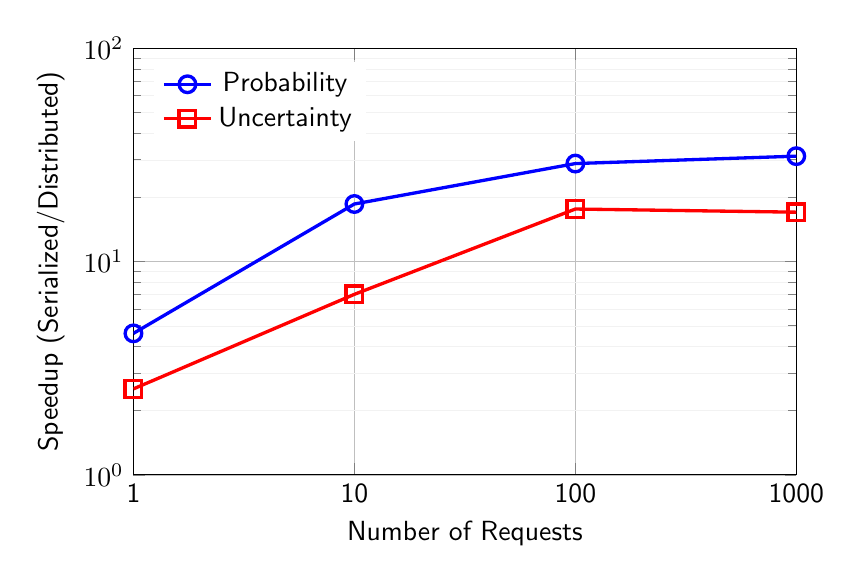
\begin{tikzpicture}
        \begin{loglogaxis}[
            width=10cm,
            height=7cm,
            grid=both,
            minor grid style={line width=.1pt, draw=gray!10},
            major grid style={line width=.2pt, draw=gray!50},
            xlabel={Number of Requests},
            ylabel={Speedup (Serialized/Distributed)},
            legend pos=north west,
            legend style={draw=none},
            xtick={1,10,100,1000},
            xticklabels={1,10,100,1000},
            log basis x=10,
            log basis y=10,
            ymin=1, ymax=100,
            xmin=1, xmax=1000
            ]
            
            % Probability speedup data
            \addplot[
                color=blue,
                mark=o,
                line width=1.2pt,
                mark size=3pt
                ] coordinates {
                (1, 4.603)
                (10, 18.6)
                (100, 28.776)
                (1000, 31.167)
            };
            
            % Uncertainty speedup data
            \addplot[
                color=red,
                mark=square,
                line width=1.2pt,
                mark size=3pt
                ] coordinates {
                (1, 2.528)
                (10, 7.016)
                (100, 17.616)
                (1000, 17.029)
            };
            
            \legend{Probability, Uncertainty}
        \end{loglogaxis}
    \end{tikzpicture}
    \caption{Speedup comparison between serialized and distributed execution for different request volumes.}
    \label{fig:speedup}
\end{figure}

The super-linear speedup for single request workloads is caused by the elimination of I/O processes. In the serialized \texttt{scram-cli} baseline, each run must (i) parse command-line arguments, (ii) read and validate the input XML fault-tree, (iii) launch a new process to execute the solver, and (iv) synchronously write results back to disk. In the distributed implementation, the request payload already contains the model and run-time parameters, which are passed directly to a Node.js native addon that invokes the underlying \texttt{scram} library. Result persistence is off-loaded to an asynchronous database writing process. So, both the initial XML parsing and the final file output are effectively removed from the process. Consequently, execution time reflects only the core solver computation, producing the observed speed-ups ($S\approx4.6$ for probability estimation and $S\approx2.5$ for uncertainty analysis) even at a single concurrent request.  
Beyond 100 jobs, speed-up saturates owing to:

\begin{itemize}
  \item \textbf{Worker saturation}: eight containers fully occupy the host's 8 hardware threads; adding jobs only increases wait time.
  \item \textbf{Queue latency}: larger batches incur longer residence times in RabbitMQ prior to dispatch.
  \item \textbf{Memory bandwidth limits}: uncertainty calculations are memory-bound; waiting time grows with concurrency.
\end{itemize}

These findings validate that the combined architecture of Docker-Swarm and RabbitMQ delivers near-linear scaling for practical PRA workloads up to the tested concurrency and provides an order-of-magnitude reduction in wall-clock time compared with serialized execution.
}

% \section{Handling Multi-Hazard Models in Parallel}
% \subsection{Integration of Hazard Modules}
% \subsection{Numerical Stability and Overflow Handling}

% \section{Security and Data Ownership}
% \subsection{Data Sharing Protocols}
% \subsection{Access Control and Regulatory Constraints}
\chapter{Building a Data-Parallel Monte Carlo Probability Estimator}

To handle massively parallel Monte Carlo evaluations of large-scale Boolean functions, we have developed a preliminary layered architecture that organizes computation in a topological graph. At the lowest level, each Boolean variable/basic event (e.g., a component failure) is associated with a random number generator to sample its truth assignment. We bit-pack these outcome, storing multiple Monte Carlo samples in each machine word to maximize computational throughput and reduce memory footprint. Subsequent layers consist of logically higher gates or composite structures that receive the bit-packed results from previous layers and combine them in parallel using coalesced kernels. By traversing the computation graph topologically, dependencies between gates and events are naturally enforced, so kernels for each layer can run concurrently once all prerequisite layers finish, resulting in high kernel occupancy and predictable throughput.
In practice, each layer is dispatched to an accelerator node using a data-parallel model implement using \acrshort{sycl}. The random number generation pipelines are counter-based, ensuring reproducibility and thread-safety even across millions or billions of samples. Gates that go beyond simple AND/OR logic--such as \acrshort{vot} operators--are handled by specialized routines that can exploit native popcount instructions for efficient threshold evaluations. As we progress upwards through the layered topology, each gate or sub-function writes out its bit-packed output, effectively acting as an input stream to the next layer.
Throughout the simulation, online tallying kernels aggregate how often each node or gate evaluates to True. These tallies can then be turned into estimates of probabilities and sensitivity metrics on the fly. This approach also makes adaptive sampling feasible: if specific gates appear to dominate variance or are tied to particularly rare events, additional sampling can be allocated to their layer to refine estimates.


\section{Layered Topological Organization}
\label{sec:layered_dag_traversal}

Recall that a \acrshort{pdag} \(\mathcal{G} = (\mathcal{V}, \mathcal{E})\) contains no cycles, so there is at least one valid \emph{topological ordering} of its nodes.  A topological ordering assigns each node a numerical \emph{layer index} such that all edges point from a lower-numbered layer to a higher-numbered layer. If a node \(v\) consumes the outputs of nodes \(\{u_1,\dots,u_k\}\), then we require
\[
\text{layer}(u_i) \;<\; \text{layer}(v)
\quad
\text{for each }i\in\{1,\dots,k\}.
\]
In other words, node \(v\) can appear only after all of its inputs in a linear or layered listing.

The essential steps to build and traverse these layers are:

\begin{enumerate}
    \item \emph{Compute Depths via Recursive Analysis:}  
      Each node's depth is found by inspecting its children (or inputs).  If a node is a leaf (e.g., a \texttt{Variable} or \texttt{Constant} that does not depend on any other node), its depth is 0.  Otherwise, its depth is one larger than the maximum depth among its children.  

    \item \emph{Group Nodes by Layer:}  
      Once each node's depth is computed, nodes of equal depth form a single \emph{layer}. Thus, all nodes with depth \(0\) are in the first layer, those with depth \(1\) in the second layer, and so on.  

    \item \emph{Sort Nodes within Each Layer:}  
      Within each layer, enforce an additional consistent ordering: (i)~variables appear before gates, (ii)~gates of different types can be grouped to facilitate specialized processing.  This step is not strictly required for correctness, but it can streamline subsequent stages such as kernel generation or partial evaluations.

    \item \emph{Traverse Layer by Layer:}  
      A final pass iterates over each layer in ascending order.  Because all inputs of any node in layer \(d\) lie in layers \(< d\), the evaluation (or "kernel build") for layer \(d\) can proceed after the entire set of layers \(0,\dots,d-1\) is processed.
\end{enumerate}

This structure ensures a sound evaluation of the \acrshort{pdag}: no gate or variable is computed until after all of its inputs are finalized.

\subsection{Depth Computation and Node Collection}

\begin{enumerate}
    \item \textbf{Clear Previous State.}  
      Any existing "visit" markers or stored depths in the \acrshort{pdag}-based data structures are reset to default values (e.g., zero or -1).
      
    \item \textbf{Depth Assignment by Recursion.}  
      A \texttt{compute\_depth} subroutine inspects each node:
      \begin{enumerate}
        \item If the node is a \texttt{Variable} or \texttt{Constant}, it is a leaf in the \acrshort{pdag}, so depth \(=0\).  
        \item If the node is a \texttt{Gate} with multiple inputs, the procedure first recursively computes the depths of its inputs. It then sets its own depth as 
        \[
          \text{depth}(\texttt{gate})
          \;=\;
          1 \;+\;\max\limits_{\ell \in \text{inputs of gate}} \Bigl[\text{depth}(\ell)\Bigr].
        \]
      \end{enumerate}
    \item \textbf{Order Assignment.}  
      Each node stores the newly computed depth in an internal field. This numeric value anchors the node to a layer. A consistent pass over the entire graph ensures correctness for all nodes.
\end{enumerate}

After depths are assigned, gather all nodes, walking the \acrshort{pdag} from its root, recording each discovered node and adding it to a global list.

\subsection{Layer Grouping and Local Sorting}

Begin by creating:
\begin{itemize}
\item A global list of all nodes, each with a valid depth,  
\item A mapping from node indices to node pointers,  
\end{itemize}
Then, sort the global list by ascending depth.  Let \(\text{order}(n)\) be the depth of node \(n\).  Then
\[
\text{order}(n_1)\;\le\;\text{order}(n_2)\;\le\;\dots\,\le\;\text{order}(n_{|\mathcal{V}|}).
\]
Finally, partition this list into contiguous \emph{layers}: if the deepest node has a depth \(\delta_{\max}\), then create sub-lists:
\[
\{\text{nodes s.t. depth}=0\},
\quad
\{\text{nodes s.t. depth}=1\},
\quad
\dots,
\quad
\{\text{nodes s.t. depth}=\delta_{\max}\}.
\]
Within each layer, sort nodes to ensure that \texttt{Variable} nodes precede \texttt{Gate} nodes, and \texttt{Gate} nodes may be further sorted by \texttt{Connective} type (e.g., \texttt{AND}, \texttt{OR}, \texttt{VOT}, etc.).

\subsection{Layer-by-Layer Kernel Construction}

Apply the layer decomposition to drive \emph{kernel building} and \emph{evaluation}:

\begin{enumerate}
    \item \textbf{Iterate over each layer in ascending depth}.  Because every node's dependencies lie in a strictly lower layer, one is guaranteed that those dependencies have already been assigned memory buffers, partial results, or other necessary resources.
    \item \textbf{Partition the layer nodes into subsets by node type}.  Concretely, \texttt{Variable} nodes are batched together for \emph{basic-event sampling} kernels, while \texttt{Gate} nodes are transferred into \emph{gate-evaluation} kernels.  
    \item \textbf{Generate device kernels}.  For \texttt{Variable} nodes, create Monte Carlo sampling kernels. For \texttt{Gate} nodes, it constructs logical or bitwise operations that merge or transform the sampled states of the inputs.  
\end{enumerate}

Once kernels for a given layer finish, move on to the next layer. Because of the topological guarantee, no node in layer \(d\) references memory or intermediate states from layer \(d\!+\!1\) or later, preventing cyclical references and ensuring correctness.
\section{Bitpacked Random Number Generator}

Monte Carlo simulations, probability evaluations, and other sampling-based procedures benefit greatly from efficient, high-quality \acrfull{rng}s. A large class of modern \acrshort{rng}s are known as \textit{counter-based \acrfull{prng}s}, because they use integer counters (e.g., 32-bit or 64-bit) along with a stateless transformation to produce random outputs. The \emph{Philox} family of counter-based \acrshort{prng}s is a well-known example, featuring fast generation, high period, and good statistical properties. In this section, we discuss the general principles of counter-based \acrshort{prng}s, explain how Philox fits into this paradigm, analyze its complexity, and present a concise pseudocode version of the \(\text{Philox }4\times32\text{-10}\) variant. Subsequently, we detail the bitpacking scheme used to reduce memory consumption when storing large numbers of Bernoulli samples.

A counter-based \acrshort{prng} maps a user-supplied \emph{counter} (plus, optionally, a \emph{key}) to a fixed-size block of random bits via a deterministic function. Formally, if 
\[
  \mathbf{x} \;=\; (x_1, x_2, \ldots, x_k)
\]
is a vector of one or more 32-bit or 64-bit counters, and 
\[
  \mathbf{k} \;=\; (k_1, k_2, \ldots, k_m)
\]
is a key vector, then a counter-based \acrshort{prng} defines a transformation 
\[
   \mathcal{F}(\mathbf{x}, \mathbf{k})
   \;=\;
   (\rho_1, \rho_2, \ldots, \rho_r),
\]
where each \(\rho_j\) is typically a 32-bit or 64-bit output. Different increments of the counter \(\mathbf{x}\) produce different pseudo-random outputs \(\rho_j\). The process is stateless in the sense that advancing the RNG amounts to incrementing the counter (e.g., \(\mathbf{x}\mapsto \mathbf{x} + 1\)).

Compared to older recurrence-based \acrshort{rng}s such as linear congruential generators or the Mersenne Twister, counter-based methods offer more straightforward parallelization, reproducibility across multiple streams, and strong structural simplicity: no internal state must be updated or maintained. This is particularly valuable in distributed Monte Carlo simulations or \acrshort{gpu}-based sampling, where each thread or work-item can be assigned a different counter. Philox constructs its pseudo-random outputs by applying a small set of mixed arithmetic (multiplication/bitwise) rounds to an input \emph{counter} plus \emph{key}. In particular, \(\mathrm{Philox}\,4\times32\text{-10}\) (often shortened to "Philox-4x32-10”) works on four 32-bit integers at a time:
\[
  \mathbf{S} = (S_0, S_1, S_2, S_3),
  \qquad
  \mathbf{K} = (K_0, K_1).
\]
The four elements \(\{S_0, S_1, S_2, S_3\}\) collectively represent the counter, e.g., \((x_0, x_1, x_2, x_3)\). The two key elements \((K_0, K_1)\) are used to tweak the generator's sequence. A single invocation of Philox-4x32-10 transforms \(\mathbf{S}\) into four new 32-bit outputs after ten rounds of mixing. At each round, the algorithm:
\begin{enumerate}
    \item Multiplies two of the state words by fixed "magic constants” to create partial products.
    \item Takes the high and low 32-bit portions of those 64-bit products.
    \item Incorporates the round key to shuffle the words.
    \item Bumps the key by adding constant increments \((\mathrm{W32A} = 0x9E3779B9 \text{ and } \mathrm{W32B} = 0xBB67AE85)\).
\end{enumerate}
After ten rounds, the final \((S_0, S_1, S_2, S_3)\) is returned as the pseudo-random block. A new call to Philox increases the counter \(\mathbf{S}\) by one (e.g., \(S_3 \mapsto S_3 + 1\)) and re-enters the same function. The Philox-4x32-10 algorithm is designed so that each blocking call requires a \emph{constant number} of operations, independent of the size of any prior "state.” Specifically, each round involves:
\[
  \mathcal{O}(1)\;\text{ arithmetic operations},
\]
and there are \(\mathrm{R} = 10\) rounds. Thus, each Philox invocation is asymptotically constant time \(\mathcal{O}(\mathrm{R}) = \mathcal{O}(1)\). The total cost to generate 128 bits (4 words \(\times\) 32 bits) is therefore constant time per call.

\subsection{The 10-round Philox-4x32}
Our implementation follows the standard 10-round approach for generating one block of four 32-bit random words, also called Philox-4x32-10. Let \(M_{\mathrm{A}}=0xD2511F53\), \(M_{\mathrm{B}}=0xCD9E8D57\) be the multipliers, and let \((K_0, K_1)\) be the key which is updated each round by \(\mathrm{W32A}=0x9E3779B9\) and \(\mathrm{W32B}=0xBB67AE85\). The function \(\text{Hi}(\cdot)\) returns the high 32 bits of a 64-bit product, and \(\text{Lo}(\cdot)\) returns the low 32 bits. Because each call produces four 32-bit pseudo-random words, Philox-4x32-10 is particularly convenient for batched sampling. If only a single 32-bit word is needed, one can still call the function and discard the excess words; however, many applications consume all four outputs (e.g., to produce four floating-point variates).

\begin{algorithm}[ht]
  \caption{Philox-4x32-10}\label{alg:philox}
  \begin{algorithmic}[1]
    %------------------------------------------------------------
    \Require Four 32-bit counters $(S_0,S_1,S_2,S_3)$,
            key $(K_0,K_1)$
    \Ensure  Transformed counters $(S_0,S_1,S_2,S_3)$
    %------------------------------------------------------------
    \Statex
    %--------------------- Philox_Round -------------------------
    \Procedure{Philox\_Round}{$(S_0,S_1,S_2,S_3),\,(K_0,K_1)$}
      \State $P_0 \gets M_{\text{A}}\times S_0$ \Comment{64-bit product}
      \State $P_1 \gets M_{\text{B}}\times S_2$ \Comment{64-bit product}
      \State $T_0 \gets \mathrm{Hi}(P_1)\,\oplus\,S_1\,\oplus\,K_0$
      \State $T_1 \gets \mathrm{Lo}(P_1)$
      \State $T_2 \gets \mathrm{Hi}(P_0)\,\oplus\,S_3\,\oplus\,K_1$
      \State $T_3 \gets \mathrm{Lo}(P_0)$
      \State $K_0 \gets K_0 + \mathrm{W32A}$
      \State $K_1 \gets K_1 + \mathrm{W32B}$
      \State \Return $\bigl((T_0,T_1,T_2,T_3),\,(K_0,K_1)\bigr)$
    \EndProcedure
    %------------------- Philox4x32_10 --------------------------
    \Statex
    \Procedure{Philox4x32\_10}{$(S_0,S_1,S_2,S_3),\,(K_0,K_1)$}
      \For{$i \gets 1$ \textbf{to} 10}
        \State $\bigl(S_0,S_1,S_2,S_3),\,(K_0,K_1) \gets$
               \Call{Philox\_Round}{$(S_0,S_1,S_2,S_3),\,(K_0,K_1)$}
      \EndFor
      \State \Return $(S_0,S_1,S_2,S_3)$
    \EndProcedure
  \end{algorithmic}
\end{algorithm}

\subsection{Bitpacking for Probability Sampling}
It takes exactly one bit to represent the outcome of a trial. If these If outcomes are stored naively, each one occupies a full 8-bit byte. Hence, only \( \tfrac{1}{8} \) of the allocated space is used for actual data. By instead packing up to \(w\) indicators into a \(w\)-bit machine word, the memory usage can be reduced by a factor of up to \(8\) (in the simplest scenario of 8-bit groupings). In more general terms:
\[
  \text{Memory usage }M_{\text{naive}}
  \;=\;
  N \times 8\;\text{bits},
  \qquad
  \text{Memory usage }M_{\text{pack}}
  \;=\;
  \left\lceil\frac{N}{w}\right\rceil \,\times\,w\;\text{bits}.
\]
In our implementation, each call to Philox-4x32-10 yields 128 bits of randomness. We use those bits to draw exactly 128 Bernoulli outcomes at once, then combine them into a \(\mathrm{bitpack}\) of two 64-bit integers. For instance, if we choose a batch size of \(4\)-bits to represent four Bernoulli samples in a single chunk, we can:

\begin{enumerate}
    \item Generate a block \(\{r_0, r_1, r_2, r_3\}\) of four 32-bit random integers from Philox.
    \item Convert each \(r_i\) into a uniform \([0,1)\) floating-point value by dividing by \(2^{32}\).
    \item Compare each to the target probability \(p\).
    \item Form a 4-bit integer, each bit set to \(1\) if the corresponding comparison succeeded, or \(0\) otherwise.
\end{enumerate}

Repeating these steps for multiple rounds of 4 bits each can fill a 16-bit or 32-bit \(\mathrm{bitpack}\) variable with many Bernoulli indicators. Then it can be stored into an array at a single index, reducing memory overhead by constant factor of $N$. 

\begin{algorithm}[H]
  \caption{Bit-packing of four Bernoulli samples into a 4-bit block}
  \label{alg:four_bit_pack}
  \begin{algorithmic}[1]
    %------------------------------------------------------------
    \Require Probability $p\in[0,1]$, random 32-bit words $(r_0,r_1,r_2,r_3)$
    \Ensure  4-bit integer bits containing the four Bernoulli draws
    %------------------------------------------------------------
    \Procedure{FourBitPack}{$p,(r_0,r_1,r_2,r_3)$}
      \State bits $\gets 0$
      \For{$i \gets 0$ \textbf{to} 3}
        \State $u_i \gets r_i / 2^{32}$ \Comment{$u_i\in[0,1)$}
        \If{$u_i < p$}
            \State $b_i \gets 1$
        \Else
            \State $b_i \gets 0$
        \EndIf
        \State bits $\gets$ bits $\mid (b_i \ll i)$ 
               \Comment{set bit $i$ to $b_i$}
      \EndFor
      \State \Return bits
    \EndProcedure
  \end{algorithmic}
\end{algorithm}

In this procedure, \(\Vert\) denotes a bitwise OR, and \(\ll\) denotes a left shift. One then repeats the above call to accumulate multiple 4-bit blocks (e.g., for a total of 16 bits, one calls FourBitPack four times and merges the results with the appropriate shifts).
\section{Tallying Layer Outputs}
\label{sec:tally_kernel}

At every Monte-Carlo iteration the simulator produces, for each logic node
\(v\in \mathcal{V}\), a bit-packed buffer encoding
\[
  \mathbf{Y}_v^{(t)}
  \;=\;
  \bigl(y_{v,1}^{(t)}, y_{v,2}^{(t)},\dots, y_{v,N}^{(t)}\bigr)
  \in\{0,1\}^N,
  \quad t = 1,\dots,T,
\]
where \(N\!=\!B\!\times\!P\!\times\!\omega\) is the number of Bernoulli trials
per Monte-Carlo \emph{iteration}:
\begin{itemize}
    \item \(B\) - number of \emph{batches},
    \item \(P\) - bit-packs per batch,
    \item \(\omega\!=\!8\cdot\mathrm{sizeof}(\text{bitpack\_t})\) - bits per pack.
\end{itemize}
Because the buffers are overwritten at the next iteration, a
separate \emph{tally layer} accumulates summary statistics that persist for the
entire simulation.  The present section formalises that process and outlines
an implementation-agnostic, data-parallel algorithm that realises it on modern
accelerators.

\subsection{Statistical Objectives}
\label{subsec:tally_objective}

For every node \(v\) we wish to estimate, after \(T\) Monte-Carlo iterations,

\[
  \widehat{p}_v
  \;=\;
  \frac{1}{T\,N}
  \sum_{t=1}^{T}\sum_{j=1}^{N} y_{v,j}^{(t)}
  \;=\;
  \frac{s_v}{T\,N},
  \qquad
  s_v \;=\; \text{total \# of one-bits observed for node \(v\)}.
\]

Under the usual independence assumptions, the sampling distribution of
\(\widehat{p}_v\) is asymptotically
\[
\mathcal{N}\!\bigl(p_v,\,
  \tfrac{p_v(1-p_v)}{T\,N}\bigr)
\]
Hence

\[
  \widehat{\sigma}_v
  \;=\;
  \sqrt{\frac{\widehat{p}_v\,(1-\widehat{p}_v)}{T\,N}}
\]

is an unbiased estimator of the standard error, giving the
\((1-\alpha)\)\,--\,level normal confidence interval

\[
  \bigl[
    \widehat{p}_v - z_{1-\alpha/2}\,\widehat{\sigma}_v,\;
    \widehat{p}_v + z_{1-\alpha/2}\,\widehat{\sigma}_v
  \bigr],
  \qquad
  z_{1-\alpha/2}\in\{1.96,\,2.58,\dots\}.
\]

The tally routine therefore needs to maintain only the scalar
\(s_v\) while the simulation is running; the derived statistics can be updated
in-place whenever a user requests intermediate results or at a fixed cadence.

\subsection{Parallel Accumulation Algorithm}

The accumulation kernel is invoked on a three-dimensional
\texttt{nd\_range}, chosen such that
\[
  \begin{aligned}
    \text{global}_x &\;\ge\; V,\\
    \text{global}_y &\;\ge\; B,\\
    \text{global}_z &\;\ge\; P.
  \end{aligned}
\]
Work-item \((i_x,i_y,i_z)\) is responsible for \emph{exactly one} bit-pack:
\[
  \text{node  } v=i_x,\quad
  \text{batch } b=i_y,\quad
  \text{pack  } p=i_z.
\]

\vspace{4pt}
\noindent
\textbf{Local workflow of a work-item}
\begin{enumerate}
    \item Load the \(p^{\text{th}}\) bit-pack of batch \(b\) from
          \texttt{buffer}.
    \item Compute \(c=\mathrm{popcount}(\text{bitpack})\).
    \item Reduce the \(c\)'s belonging to the same work-\emph{group} in
          shared memory (tree reduction or \texttt{reduce\_over\_group}).
    \item One designated leader performs
          \(\texttt{atomic\_add}(\texttt{num\_one\_bits},\,\text{group\_sum})\).
\end{enumerate}

The reduction ensures only one atomic operation per group, greatly reducing
contention when \(P\) is large.

We present platform-neutral pseudocode that encapsulates the above logic while remaining agnostic to the underlying API. After each Monte-Carlo iteration the host enqueues \textsc{TallyKernel} with a
fresh \texttt{iteration} counter.  When either (i)~a user requests
intermediate statistics or (ii)~a pre-set reporting interval is reached,
the host reads back \texttt{num\_one\_bits} and executes the purely
serial routine shown in Algorithm~\ref{alg:update_stats}.

\begin{algorithm}[H]
\caption{Post-processing of a single node's tally}
\label{alg:update_stats}
\begin{algorithmic}[1]
  \Require
    \(s\) - total one-bits,
    \(T\), \(B\), \(P\), \(\omega\) - run parameters
  \Ensure
    \(\widehat{p}\), \(\widehat{\sigma}\), two symmetric CIs
  \State $N\gets B\cdot P\cdot\omega$
  \State $\widehat{p}\gets s / (T\,N)$
  \State $\widehat{\sigma}\gets
          \sqrt{\widehat{p}(1-\widehat{p})/(T\,N)}$
  \For{\textbf{each} $z\in\{1.96,\,2.58\}$}
      \State $\text{CI}\gets
        \bigl[\max(0,\widehat{p}-z\widehat{\sigma}),
              \min(1,\widehat{p}+z\widehat{\sigma})\bigr]$
  \EndFor
\end{algorithmic}
\end{algorithm}

The above normal approximation is valid provided \(T\,N\widehat{p}\)
and \(T\,N(1-\widehat{p})\) both exceed roughly 10; otherwise an exact
Clopper-Pearson interval can be substituted with no change to the running
sum logic.

\subsection{Correctness and Complexity}

\textbf{Work-item cost.}
Each work-item performs one \(\mathrm{popcount}\) and
participates in an \(O(\log L)\) intra-group reduction
(\(L\!=\!\text{local\_range}\)), yielding an overall
\(O(\log L)\) instruction count.

\textbf{Global cost.}
The total number of work-items launched per iteration is
\(V\cdot B\cdot P\).  Because each bit-pack contains \(\omega\) Bernoulli
trials, the cost \emph{per trial} shrinks as \(\omega^{-1}\).

\textbf{Memory traffic.}
Every work-item reads exactly one machine word and no writes occur except
the single atomic addition per work-group.  Hence the algorithm is
memory-bandwidth bound only at extremely low arithmetic intensity
(\(P\approx 1\)).

\textbf{Linear scalability.}
All tally nodes are independent.  Increasing \(V\) therefore scales the total
runtime linearly until either (i)~the device saturates its occupancy or
(ii)~atomic contention becomes non-negligible; the group-level reduction
mitigates the latter.

\section{Preliminary Benchmarks on Arialia Fault Trees}
\input{4_proposed_solution/mc_solver/benchmarks/setup}
\input{4_proposed_solution/mc_solver/benchmarks/results_accuracy}
\input{4_proposed_solution/mc_solver/benchmarks/results_mem_runtime}
\input{4_proposed_solution/mc_solver/benchmarks/limitations}

{
\cleardoublepage
\let\clearpage\relax
\include{4_proposed_solution/overview/_}

\chapter{Designing a Distributed Queuing System}

\section{Worker-Pool and Queue Management Concepts}

The distributed system follows a \emph{publisher--consumer} pattern. In this architecture, a \textbf{publisher} is typically a client-facing service, such as REST \acrshort{api}s, responsible for receiving requests from front-end clients and forwarding these requests to an exchange inside a message broker. A \textbf{message broker} is a middleware system that facilitates communication between publishers and consumers by routing messages.

Within the broker, the \textbf{exchange} component directs each request to an appropriate queue based on the routing key of the request. A \textbf{queue} is a data structure within the broker that temporarily stores messages until they are processed by consumers. Each queue is configured with specific user-defined settings, such as message time-to-live, maximum queue length, and prefetch limits (the maximum number of messages that a consumer can process simultaneously).

A \textbf{scheduler} layer adds service-level metadata to these messages, including priority, delays, and enforces ordering policies such as \acrshort{fifo} or strict priority ordering. \acrshort{fifo} ensures that messages are processed in the order they arrive, while strict priority ordering processes messages based on assigned priority levels. Queues can be marked as durable, enabling recovery of messages in case of broker restarts or failures. Messages can be marked as persistent, guaranteeing delivery despite network or consumer disruptions. Additionally, queues support a \textbf{dead-letter queue} mechanism, a specialized queue that captures undeliverable or failed messages, allowing for subsequent analysis and recovery operations.

A \textbf{consumer} represents any \acrshort{pra} solver instance within the worker pool. The \textbf{worker pool} is essentially a collection of solver processes running on \acrshort{cpu}s, \acrshort{gpu}s, or \acrshort{fpga}s. These consumers connect to their designated queues and consume messages based on prefetch settings. Consumers process each message by retrieving the \acrshort{pra} models and solver parameters from the message body. Then they perform calculations and persist the results in the distributed databases. Upon successful completion, they send an \textbf{acknowledgement}, a confirmation message indicating successful processing, back to the broker, marking the message as processed.

The broker implements idempotent operations, meaning duplicate or repeated actions are processed only once. For example, if the user repeatedly attempts to create a queue, the broker will create the queue once and ignore the rest of the repeated commands. Finally, both publishers and consumers send periodic heartbeats, regular signals or pings, to the broker to ensure the active status of these components. These heartbeats allow the developers to monitor service availability and manage the health of the distributed system. Figure \ref{fig:worker-pool-queue-management} shows a basic publisher-consumer workflow of a message broker.

\input{4_proposed_solution/dist_queues/plots/plot_dist_msg_broker}

\section{REST APIs for Parallel Task Coordination}

The platform provides a RESTful \acrshort{api} layer that orchestrates the entire life cycle of \acrshort{pra} quantification tasks, from submission and monitoring to cancellation and result retrieval. An \acrshort{api} is a set of rules that lets different software systems exchange data programmatically over the internet. A RESTful \acrshort{api} implements these rules using standard \acrshort{http} methods (GET, POST, PUT, DELETE) and resource-oriented \acrshort{url}s to ensure stateless communication. The REST \acrshort{api}s handles client authentication and payload validation, translating task definitions (\acrshort{pra} models and solver parameters) into messages dispatched to the publisher component of the distributed system. Upon successful POST, clients receive a unique task identifier, which they use to subscribe to status endpoints to get real-time execution updates (queued, running, completed, failed). Batch submission endpoints accept arrays of quantification tasks with optional metadata for target solver selection (\acrshort{mocus}/\acrshort{bdd}/\acrshort{zdd}/Monte Carlo), priority levels, and estimated resource requirements. Result endpoints expose completed outputs and solver performance metrics in \acrshort{json} format via secure download \acrshort{url}s pointing to the distributed databases. To ensure fair usage, the \acrshort{api}s implement idempotent POST semantics and rate limiting to prevent duplicate requests and resource starvation. Figure \ref{fig:rest-api-architecture} shows a simplified workflow of the REST API layer.

\input{4_proposed_solution/dist_queues/plots/plot_dist_rest_api}

\section{Design of the Distributed System}

\subsection{Load Balancing and Scheduling}

The distributed architecture is designed to handle a high volume of concurrent PRA quantification tasks with minimal latency and maximum resource utilization. To achieve this, the system employs containerization and cluster orchestration to distribute workloads across multiple computing nodes, combined with scheduling policies to balance the load. Quantification jobs are managed through a message-queue system that decouples task submission from execution, enabling tasks to be executed in parallel by a pool of workers. The framework statically scales the number of worker instances before launch and assigns each job type to its own queue. This scheduling approach reserves resources for every class of quantification task and enables rapid deployment of additional workers when larger models--or large-scale studies--must be processed. Core strategies include (i) distributing tasks across dedicated queues in a Docker Swarm cluster, (ii) using a multi-queue workload manager, (iii) partitioning complex models into parallel tasks, and (iv) adaptively selecting algorithms for each stage of the analysis. These measures collectively provide efficient load balancing and scheduling for the platform's quantification engine.

\subsection{Distributed Task Scheduling in the Cluster}

The distributed queuing system is structured as two loosely coupled, independently deployable microservices within a mono repository: one implements the publisher service, and the other implements the consumer service. These microservices are then deployed as Docker services across a Docker swarm cluster \cite{Swarm}. The cluster consists of a manager node and multiple worker nodes. The manager node is responsible for orchestrating operations and maintaining the cluster state (e.g., monitoring node health and resource usage), while the workers execute the quantification tasks. Both the backend producer service and the worker (consumer) service are containerized as separate Docker  images. The producer service (running on one or more instances) handles incoming analysis requests. It runs the NestJS-based backend \cite{Documentation} and connects to RabbitMQ \cite{RabbitMQ} and the MongoDB \cite{MongoDB} database, and the worker service encapsulates the scram \cite{scram} quantification engine via its Node.js NAPI \cite{Node} bindings, along with its own RabbitMQ client and database access.

When a user submits a model for quantification (for example, by clicking “Quantify” in the web editor or via a REST API call), an HTTP request with the model data and analysis parameters is sent to the backend (producer) service. To avoid sending large files over the network or through the message queue, the backend stores the model input (OpenPSA MEF XML files \cite{2017OpenPSAMEF}) in the MongoDB database and retains only a document ID. The request is then tagged with metadata including the document ID and the requested analysis type. At this point, a priority level is assigned based on the analysis type or urgency of the task. For instance, a simple point estimate might be treated as high priority, whereas a lengthy uncertainty propagation could be set as lower priority. The producer then serializes the task description including the document ID and priority into a message and enqueues it into a RabbitMQ job queue. RabbitMQ serves as the central task broker -- it enables asynchronous handling of potentially thousands of jobs without overloading the web server, and it routes tasks to available workers. If multiple producer instances are running, a Traefik \cite{Traefik} load balancer distributes incoming HTTP requests among them, preventing any single backend instance from becoming a bottleneck and thereby balancing the load at the entry point of the system.

On the execution side, a fleet of worker containers run on the Swarm cluster's worker nodes to perform the actual model quantifications. The manager node can scale the number of active worker containers up or down (currently up to 128 workers across the cluster) to match the incoming workload demand. Each worker continuously polls the RabbitMQ queue for new jobs. RabbitMQ supports multiple queues, so jobs can be segregated by priority or type, and the workers always draw the highest priority jobs first from their individual queues. Once a worker retrieves a job message, it fetches the corresponding model input data from MongoDB (using the document ID in the message), then invokes the scram engine via the Node.js native addon to perform the quantification. By containerizing the scram engine and associated libraries, the system isolates each task's execution while allowing it to fully utilize a CPU core (or multiple cores if the engine itself is multi-threaded) on the worker node. After the quantification completes, the worker saves the output (results files, logs, etc.) back to the database, associating them with the same document ID for later retrieval. It then sends an acknowledgment to RabbitMQ so that the message is removed from the queue. The platform uses RabbitMQ's manual acknowledgment mechanism: a task message is only cleared from the queue when a worker signals successful completion. If a worker crashes or fails before finishing, the lack of acknowledgment causes RabbitMQ to automatically re-queue the task, making it available for another worker to pick up. \emph{Figure~\ref{fig:distributed-workflow}} illustrates this distributed workflow: multiple producers accept user requests and queue tasks, and a pool of workers on the cluster consume tasks, quantify and return results.

\input{4_proposed_solution/dist_queues/plots/plot_dist_workflow}

\subsection{Multi-Queue Workload Management}
\label{subsec:multi-queue}

The system currently employs a multi-queue architecture that routes requests according to solver execution mode. The worker replicas are statically scaled up (or down), so the cluster cannot dynamically reallocate computational resources among queues. Hence, priority-based routing is not available. Only intra-queue priorities are ensured, meaning higher-priority messages within a queue are processed before lower-priority ones. All queues are hosted in the same RabbitMQ broker, but each provides messages to a distinct worker deployment and calls a different execution pathway inside the cluster.

\paragraph{Queue type~1: API--Model jobs}
This type of queue is used when a client sends an \textsc{http} \texttt{POST} request to \texttt{/quantify} endpoint. The request contains the PRA model in Base64 form (the payload is an OpenPSA MEF XML file, converted to a single Base64 string) together with the chosen solver name (\texttt{scram-bdd}, \texttt{scram-mocus}, \texttt{scram-mc} etc.) and any run parameters. The producer service stores the raw model in MongoDB, inserts the \texttt{model id} along with solver parameters into a JSON task document, and publishes that document to the queue.  A pool of \texttt{model worker} containers subscribes exclusively to this queue.

Each worker:

\begin{enumerate}
  \item Retrieves the task, downloads the model blob from MongoDB, and
        writes it to a temporary file inside the container.
  \item Invokes the designated solver on that file.
  \item Persists the results back to the database and acknowledges the message.
\end{enumerate}

Since the model travels with the message, these jobs are fully self-contained and the cluster does not require shared storage.

\paragraph{Queue~2: API--Exec jobs}
When the client prefers not to embed the PRA model in the request payload, the solver can be invoked as a shell command within a working directory that already contains the input files. In this case, the client sends an HTTP \texttt{POST} request to the \texttt{/execute} endpoint that specifies:

\begin{itemize}
  \item \texttt{workdir} -- the absolute path visible on the cluster where the model files reside.
  \item \texttt{cmdline} -- the exact tool invocation, identical to how the user would call it on a login node (e.g.\
  \verb|scram --mocus --mcub ft-310.xml|).
\end{itemize}

The producer wraps these two strings in a task document and publishes it
to the queue. A separate deployment of \texttt{exec worker} containers subscribes to this queue; each worker simply change directories into \texttt{workdir} and executes the given command under a limited access shell. This design keeps large input datasets out of the message queues and databases.

\subsection{Model Partitioning for Parallel Execution}

In addition to managing discrete jobs, the quantification engine employs model-specific partitioning strategies to leverage parallelism within a single large analysis. Complex PRA models -- notably, large event trees with many branching sequences or scenarios that each depend on fault tree evaluations -- are broken down into smaller sub-tasks that can be solved concurrently. Rather than treating a monolithic model as one giant quantification problem, the system identifies independent submodels (subtrees of the overall logic) and distributes those as separate jobs to the cluster. For example, consider an event tree analysis that involves hundreds of linked fault trees (one fault tree for each sequence or safety function outcome). Instead of quantifying each sequence serially, the platform treats each fault tree as an independent quantification task. All fault trees can then be processed in parallel across the distributed workers, each producing a failure probability or cut set result for its respective portion of the event tree. Once all these parallel computations are complete, a post-processing step aggregates the results: the event tree logic is applied to combine the sequence-level probabilities (or other metrics) into an overall result, which is then reported to the user as a single coherent output. This divide-and-conquer strategy acts as a pre-processing (decomposition) and post-processing (recomposition) workflow that enables the handling of extremely complex models which would be infeasible to solve in a single thread or single process. By performing dozens or hundreds of sub-calculations simultaneously, the system can significantly reduce the wall-clock time for quantifying large-scale PRA models.

One advantage of this partitioned approach is that the user can obtain interim results or a rough overview quickly, even if the full analysis is intricate. Because the most critical sub-tasks can be prioritized or because partial results become available as sub-tasks finish, the system could provide a preliminary risk estimate after the first wave of subtrees is solved, then refine that estimate as the remaining subtrees complete. In practice, the initial results might be less precise (for instance, based on a subset of scenarios or a simplified combination of outcomes), but as more computational resources come online or as more sub-tasks finish, the overall result converges to the high-accuracy answer. This means the platform can deliver a quick assessment to analysts (useful for time-sensitive decision support) and then follow up with increasingly accurate results as computation continues, effectively trading off accuracy and time. 

Moreover, the engine takes an adaptive algorithmic approach during quantification to optimize both accuracy and performance for each sub-task. Different solving algorithms excel under different conditions, so the engine can choose the most appropriate method on a per-subtask basis. For example, the MOCUS algorithm (which enumerates minimal cut sets) is very fast for low-probability scenarios but tends to lose accuracy (overestimating the top event probability) in scenarios with high component failure probabilities, due to the limitations of the rare-event approximation. On the other hand, binary decision diagram (BDD) based methods yield exact results even with higher failure probabilities but can be slower or more memory-intensive for very large logic structures. To capitalize on these strengths, the system can automatically apply a BDD-based quantification for portions of the model that involve high probability events or densely interdependent logic, while using MOCUS (potentially with approximations like the min-cut upper bound, MCUB) for other portions. In the previous example of an event tree with many fault trees, this might mean using a BDD solver for a particular fault tree known to have high-risk (high probability) contributors, and using the faster cut-set solver for fault trees in which the rare-event assumption holds. By mixing algorithms in this way, each sub-task is solved with the method best suited to its characteristics, ensuring that the final results are accurate without incurring unnecessary computational overhead.

\subsection{Handling Shared Subtrees in Distributed Memory} A particular challenge in the parallel decomposition of a PRA model is handling shared subtrees in a distributed memory environment. Shared subtrees occur when different parts of a model require the evaluation of an identical sub-model. For instance, in an event tree analysis, multiple accident sequences might involve the same mitigating system fault tree; similarly, in a large fault tree, two separate top events or portions of the logic might include a common subtree (a repeated gate structure or module). In a single-process solver, such common substructures can be computed once and reused internally to save time. However, in a distributed system each worker operates with its own memory and state, so without coordination, the same subtree could be sent to two different workers and thus be quantified twice in isolation. This would waste computational effort. The scheduling strategy avoids this by ensuring that each unique subtree is solved only once.

Before distributing tasks, the system identifies any duplicate or shared subtrees among the jobs. Rather than dispatching redundant tasks, it will assign the computation of a shared subtree to a single designated worker and hold or coordinate the dependent tasks until that worker produces the result. For example, if two event tree sequences both require the fault tree FT1, the scheduler will create a task for quantifying FT1 only once. The first sequence that needs FT1 triggers the FT1 task to be queued; the second sequence's task sees that FT1 is already in progress (or completed) and will not generate a duplicate FT1 job. When the one worker finishes solving FT1, its results (cut sets, intermediate BDD, or failure probability) are stored in a common repository -- in this case, the MongoDB database -- and indexed by an identifier (such as the subtree's ID). Then, any pending computations that depend on that subtree can retrieve the result and proceed without recomputing it.

In the event tree scenario, once fault tree FT1's probability is known, it can be plugged into all sequences that require it, and those sequences' quantifications can continue or be finalized. This mechanism effectively simulates a shared memory for that piece of data: although the cluster is distributed, the intermediate result is made available to all relevant processes through the centralized database. During the aggregation phase, the coordinator (a processed job service dedicated for aggregation process) combines the unique results from each subtree to form the overall outcome. This approach does require careful scheduling logic -- workers might need to wait for a shared dependency to be solved by another worker. This implementation is essential for large PRA models, where repeated subtrees are prevalent.

\section{Implementation of the Distributed System}

\subsection{Software Stack and Technology Selection}

\textbf{NestJS, TypeScript and RabbitMQ:} The platform uses NestJS, a Node.js based framework, with TypeScript \cite{starting} for its web services. TypeScript's static typing reduces runtime errors by validating the request and response payloads at compile time. NestJS provides a modular architecture with dependency injection and out-of-the-box support for microservices that simplifies building structured REST API based services. RabbitMQ provides all the advanced features of a message broker at no cost, while ensuring high-throughput and low latency for job processing.

\textbf{MongoDB:} Distributed MongoDB databases are used for persisting PRA models and results. MongoDB was selected for its flexible document schema and horizontal scalability (via sharding). This schema flexibility is ideal for PRA data (e.g., fault trees, event trees, Bayesian networks, etc.) which can have heterogeneous structures.

\textbf{C++ Quantification Engine (scram) and NAPI:} The quantification tasks are handled by the scram engine, written in C++. To integrate this native engine with the TypeScript language, OpenPRA employs Node's N-API (Node Addon API). N-API bridges the TypeScript and C++ layers by compiling scram's functions into a Node.js module, allowing the TypeScript code to invoke C++ quantification methods directly. This approach offers the speed of optimized C++ code while keeping the high-level logic in TypeScript, and abstracts away the complexity of the C++ codebase from the rest of the system.

\textbf{OpenMP for Multi-core Parallelism:} Within the scram engine, OpenMP is utilized to parallelize computations across multiple CPU cores. Certain analyses (e.g. uncertainty and importance measure) run in parallel threads.

\textbf{GPU Acceleration (CUDA/SYCL):} The platform also explores GPU computing to accelerate PRA analysis. Using C++ heterogeneous computing frameworks like SYCL \cite{Alpay2020SYCL}, which can target NVIDIA CUDA GPUs or other accelerators, it has been demonstrated that offloading Monte Carlo simulations to a GPU can drastically reduce computation time. Such GPU integration is considered for high-priority or large-scale simulations to further enhance throughput.

\subsection{Containerization/Virtualization Strategies}

The publisher service and the consumer service are each packaged as separate Docker container images. Docker is a widely adopted container platform that provides portable, consistent execution environments with minimal overhead. In high-performance computing environments where administrative privileges are restricted, Singularity can be utilized as an alternative container runtime. Containers share the host kernel, offering low resource usage. Docker Swarm, a container orchestration tool, manages the deployment of these containers across multiple nodes. The manager node schedules services and maintains cluster states. A Traefik load balancer distributes incoming REST \acrshort{api} requests evenly among publisher instances. Dedicated computing nodes are connected by high-speed interconnects (such as high-speed Ethernet) ensuring low-latency communications.

Resource allocation and management are orchestrated through a declarative configuration defined in a Docker Compose file, which specifies service deployment, network connectivity, resource constraints, and scaling policies.

Each service, including frontend interfaces, backend \acrshort{api} endpoints, job brokers, and computation workers, is deployed as a containerized application with explicit resource management policies.

\begin{itemize}
    \item \textbf{Dynamic scaling:} Services such as \texttt{job-publisher} are dynamically scaled using Docker Swarm's replicated deployment mode. This service is set up with adjustable replication factors (up to 128 replicas per node).
    
    \item \textbf{Placement constraints:} Placement constraints, defined via node labels (e.g., \texttt{host\_performance}), restrict deployment to specific nodes according to computational requirements. Resource-intensive services like \texttt{mongodb} and \texttt{rabbitmq} are constrained to nodes labeled for high performance.
    
    \item \textbf{Load balancing and scheduling:} Traefik serves as the primary load balancer, routing incoming \acrshort{http} and \acrshort{https} requests among service replicas based on predefined routing rules. Each microservice (frontend, backend, and job brokers) is configured with constraints such as \texttt{max\_replicas\_per\_node}, ensuring balanced distribution of containers across available nodes and avoiding single-node overload.
    
    \item \textbf{Update and rollback management:} Services share a unified update and rollback configuration. Updates are executed in parallel (up to 16 instances simultaneously), with rollback mechanisms triggered upon failure.
    
    \item \textbf{Resource isolation and limits:} Explicit CPU and memory constraints can be configured in the Docker Compose file to prevent resource exhaustion.
    
    \item \textbf{Health Monitoring:} Health checks are systematically performed on each service instance, using predefined intervals and thresholds to detect unhealthy containers quickly. Unresponsive or failing containers are automatically restarted.
\end{itemize}

\input{4_proposed_solution/dist_queues/deployment}

\section{Performance Evaluation and Scaling Results}
\label{sec:scaling-results}

\subsection{Experimental Setup}
\label{subsec:exp-setup}

Benchmark tests were executed on a workstation equipped with a 13\textsuperscript{th}-Gen Intel\textsuperscript{\textregistered} Core\textsuperscript{\texttrademark} i7-13700K (16 cores, 24 threads) and 32 GB RAM. Deploying the distributed system on an entry-level CPU and a single node was intentional: it demonstrates that the distributed system can run on off-the-shelf hardware without setting up a specialised network or cluster-management expertise. With fewer cores, performance-scaling plateaus appear sooner than they would on a large cluster, allowing bottlenecks to be identified earlier in the development cycle.

The \textit{baobab3.xml} fault-tree model from the Aralia fault tree data set served as the workload. Two scenarios were compared:

\begin{enumerate}
  \item \textbf{Serialized baseline:} direct invocation of \texttt{scram-cli} (single process, no queue).
  \item \textbf{Distributed system:} eight Dockerised worker containers orchestrated by Docker swarm, with jobs submitted through the REST \acrshort{api} and routed via RabbitMQ.
\end{enumerate}

End-to-end latency was measured from \textsc{http} \texttt{POST} reception to result retrieval for batches of 1, 10, 100, and 1000 concurrent requests. Two task types were profiled: point-estimate probability calculation and uncertainty quantification.

\subsection{Results and Discussion}
\label{subsec:scaling-discussion}

Table~\ref{tab:benchmark-times} lists the mean execution times (\SI{}{\second}) over four runs per workload.  
Speed-up $S$ is defined as
\input{4_proposed_solution/dist_queues/equations/eq_dist_speedup}

\input{4_proposed_solution/dist_queues/tables/table_dist_q_exec_times}

Figure~\ref{fig:speedup} depicts the resulting speed-up.  
For probability calculations the system scaled almost linearly up to 100 simultaneous jobs, peaking at $S\approx31$ for 1000 requests before reaching a plateau.  
Uncertainty quantification, which is more compute-intensive, achieved $S\approx18$ at 100 jobs, after which the speedup slightly decreased.

\input{4_proposed_solution/dist_queues/plots/plot_dist_q_speedup}

The super-linear speedup for single request workloads is caused by the elimination of I/O processes. In the serialized \texttt{scram-cli} baseline, each run must (i) parse command-line arguments, (ii) read and validate the input XML fault-tree, (iii) launch a new process to execute the solver, and (iv) synchronously write results back to disk. In the distributed implementation, the request payload already contains the model and run-time parameters, which are passed directly to a Node.js native addon that invokes the underlying \texttt{scram} library. Result persistence is off-loaded to an asynchronous database writing process. So, both the initial XML parsing and the final file output are effectively removed from the process. Consequently, execution time reflects only the core solver computation, producing the observed speed-ups ($S\approx4.6$ for probability estimation and $S\approx2.5$ for uncertainty analysis) even at a single concurrent request.  
Beyond 100 jobs, speed-up saturates owing to:

\begin{itemize}
  \item \textbf{Worker saturation}: eight containers fully occupy the host's 8 hardware threads; adding jobs only increases wait time.
  \item \textbf{Queue latency}: larger batches incur longer residence times in RabbitMQ prior to dispatch.
  \item \textbf{Memory bandwidth limits}: uncertainty calculations are memory-bound; waiting time grows with concurrency.
\end{itemize}

These findings validate that the combined architecture of Docker-Swarm and RabbitMQ delivers near-linear scaling for practical PRA workloads up to the tested concurrency and provides an order-of-magnitude reduction in wall-clock time compared with serialized execution.
}

% \section{Handling Multi-Hazard Models in Parallel}
% \subsection{Integration of Hazard Modules}
% \subsection{Numerical Stability and Overflow Handling}

% \section{Security and Data Ownership}
% \subsection{Data Sharing Protocols}
% \subsection{Access Control and Regulatory Constraints}
% \part{Code Verification and Case Studies}
% \chapter{Test Framework and Methodology}
% \section{Small-Scale Validation Models}
% \subsection{Comparison to Analytical/Exact Solutions}
% \subsection{Verification Against Simple Benchmark Fault Trees}
% 9.2 Full-Scale Validation
% 9.2.1 Large Nuclear Power Plant Case Studies
% 9.2.2 Multi-Hazard Scenarios (Seismic + Flooding, etc.)
% 9.3 Performance Benchmarking
% 9.3.1 Comparison with Legacy Tools on HPC Platforms
% 9.3.2 Scalability Analysis, Load Balancing Effectiveness

% \chapter{Results and Discussion}
% \section{Quantitative Performance Gains}
% \subsection{Speedups, Resource Utilization}
% \subsection{Sensitivity to Model Complexity}
% % \section{Accuracy and Reliability
% % 10.2.1 Validation Against Known Reference Solutions
% % 10.2.2 Error Analysis and Confidence Intervals
% \section{Lessons Learned and Limitations}
% \subsection{Addressing Numerical Instabilities}
% \subsection{Real-Time Feasibility vs. Offline Computation}


\part{Future Work}
\chapter{Directions for Ongoing and Future Research}
\section{Adaptive Scheduling for Real-Time PRA}
\section{Advanced Uncertainty Propagation}
\section{Variance Reduction Techniques}
\section{Integration with Industry Tools and Standards}




\printbibliography[
heading=bibintoc,
title={References}
]
\appendix
% \part{Foundations}
\chapter{The Triplet Definition of Risk}
\label{sec:triplet_definition_of_risk}
\input{2_foundations/definition/pra}
\input{2_foundations/definition/et/_}
\input{2_foundations/definition/ft/_}

\input{2_foundations/definition/probability/_}

\input{2_foundations/definition/mcs}
\input{2_foundations/definition/importance}
\input{2_foundations/quantification/qualitative/_}
\input{2_foundations/quantification/quantitative/_}

%\chapter{Tasks}
% \section{Task 1: Literature Review, Benchmarking, and Profiling of Current PRA Tools}
\label{sec:task1}

% \subsection{Overview of Section}
\label{sec:overview}

This section documents the completion of Task 1. The project's remaining tasks include:
\begin{itemize}
\item Task 2: Web-based \acrshort{pra} framework design and implementation
\item Task 3: Testing and benchmarking for serial and parallel improvements
\item Task 4: Applications to single hazard real-world \acrshort{pra} models
\item Task 5: Applications to multi-hazard real-world \acrshort{pra} models
\item Task 6: Verification and documentation
\end{itemize}

Following this overview, the remainder of the section is as follows:
\begin{itemize}
\item Section 3.2 summarizes the history of \acrshort{pra} tools and highlights current issues.
\item Section 3.3 introduces common \acrshort{pra} model structures.
\item Section 3.4 discusses how to quantify a model.
\item Section 3.5 provides an overview of multi-hazard \acrshort{pra} models.
\item Section 3.6 presents the benchmarking and standard profiling results for SCRAM and \acrfull{saphsolve}.
\item The section is concluded in Section 3.9.
\end{itemize}

\subsection{Probabilistic Risk Assessment Tools and Issues}
\label{sec:pra_tools_history}

In the evolution of \acrshort{pra} during the 1970s, various tools were concurrently developed to facilitate the analysis process. Below is a list of some notable \acrshort{pra} tools:

\begin{itemize}
\item \textbf{PREP and KITT} \cite{18}: Developed as computer code for automatically evaluating a fault tree by Idaho Nuclear Corporation. PREP obtains \acrshort{mcs} of the fault tree using either Monte Carlo or deterministic methods, while KITT obtains numerical probabilities associated with the tree.

\item \textbf{\acrshort{mocus}} \cite{19}: Developed by Aerojet Nuclear Company, a computer program to obtain minimal cut sets from fault trees.

\item \textbf{MODULE} \cite{20}: A computer program capable of handling minimal cut set generation, importance analysis, and uncertainty analysis.

\item \textbf{SIGPI} \cite{21}: A program developed by \acrshort{llnl} for the \acrshort{nrc} that could compute complex systems' probability.

\item \textbf{CAFTA} \cite{22}: Used to develop, maintain, and update single-top failure models using fault tree and event tree modeling techniques. It is currently maintained under the Phoenix Architect Module \cite{23} and is primarily utilized by United States \acrshort{npp} operators.

\item \textbf{SAPHIRE} \cite{24}: A follow-up work of IRRAS \cite{25,26}, developed by the \acrshort{inl} for the \acrshort{nrc}. Released in 1987, it is widely used for performing complete \acrshort{pra} on personal computers and is one of the most used \acrshort{pra} tools in the US.

\item \textbf{RISKMAN} \cite{27}: A personal computer (PC) based, general-purpose, integrated tool for quantitative risk analysis developed by ABS Consulting, Inc \cite{28}.

\item \textbf{KIRAP} \cite{29}: A fault tree construction and analysis code package.

\item \textbf{RiskSpectrum} \cite{30}: An advanced software developed by Relcon Scandpower AB, increasingly used for developing fault trees and event trees to assess system reliability in various parts of \acrshort{npp}.

\item \textbf{RiskA} \cite{31}: An integrated reliability and \acrshort{pra} tool developed by the FDS Team.

\item \textbf{XFTA} \cite{32}: A calculation engine initially developed in 2012 as part of the Open-PSA initiative.

\item \textbf{SCRAM} \cite{33}: An open-source, command-line risk analysis multi-tool currently under enhancement in the PRAG in the Nuclear Engineering Department at \acrshort{ncsu}.

\item \textbf{DeRisk} \cite{34}: A dynamic, uncertain causality graph-embedded risk analysis code package.
\end{itemize}

To summarize, numerous \acrshort{pra} tools have been developed and continuously improved. CAFTA is the preferred choice for most \acrshort{npp} operators in the US. SAPHIRE is the \acrshort{nrc}'s primary software tool for modeling, evaluating, and validating \acrshort{npp} results. Meanwhile, SCRAM is a versatile open-source \acrshort{pra} tool that can perform nearly all \acrshort{pra} calculations.

Although significant improvements have been made, there is still ample opportunity for further enhancements in \acrshort{pra} tools to utilize resources efficiently and obtain accurate results more quickly. Below are some of the current areas requiring improvement~\cite{35}:

\begin{itemize}
\item \textbf{Quantification time and efficiency}
\begin{itemize}
\item Extremely long quantification times may tax the quantification engine, leading to extended waiting periods and potential failures due to memory limitations.
\item Fire \acrshort{pra} models are significantly larger than typical internal-events models, presenting additional quantification challenges.
\end{itemize}

\item \textbf{Dependency analysis for human reliability analysis}

\item \textbf{Model development, maintenance, and updates}
\begin{itemize}
    \item Manual, labor-intensive processes are error-prone and should be automated.
    \item Model manipulation (often done through flag settings in text files) is time-consuming, inefficient, and prone to error.
\end{itemize}

\item \textbf{Risk aggregation}
\begin{itemize}
    \item \textit{Multi-hazard models:}
    \begin{itemize}
        \item Internal-events models often rely on rare-event approximations. These may be inadequate for external events such as earthquakes, high winds, and external flooding, where fragilities of Systems, Structures, and Components are typically higher.
        \item Accurate probability calculations in seismic \acrshort{pra} can quickly exhaust memory if rare-event approximations are not used.
    \end{itemize}
    \item \textit{Multi-unit sites:}
    \begin{itemize}
        \item Many current \acrshort{pra} models assume independence among units at a site, yet in practice, many resources are shared among units.
    \end{itemize}
    \item Analyzing combinations of \acrshort{pra} model elements for criticality.
    \item Uncertainty analysis:
    \begin{itemize}
        \item Most models currently apply only parametric uncertainties, lacking more detailed components.
    \end{itemize}
    \item Communication of risk insights:
    \begin{itemize}
        \item Presenting \acrshort{pra} information to non-\acrshort{pra} practitioners has been a longstanding challenge.
    \end{itemize}
    \item Incorporating new \acrshort{pra} technologies into existing models.
\end{itemize}
\end{itemize}

This project specifically addresses quantification speed, efficiency, model development, maintenance, and updates. Additionally, we discuss risk aggregation, focusing on multi-hazard \acrshort{pra} models.

% \subsection{Backgrounder on Multi-Hazard PRA}

Multi-hazard probabilistic risk assessment (PRA) addresses the challenge of analyzing multiple potential threats to a nuclear power plant (NPP) when hazards occur either concurrently or in a sequence. In general, these interactions can be complex because hazards may have non-trivial correlations or can trigger one another (e.g., a seismic event inducing a landslide). For instance, Choi et al.~\cite{Choi2021review} note that multi-hazard scenarios encompass both simultaneous and successive occurrences of distinct hazards that together can compromise plant safety. Although several approaches to multi-hazard analysis exist, no single framework is commonly adopted across the nuclear industry, resulting in varied levels of rigor and completeness.

The 2011 Fukushima Daiichi accident exemplified how multiple hazard events can combine to overwhelm existing defense-in-depth measures. According to the World Health Organization (WHO)~\cite{Great}, a magnitude 9.0 earthquake struck off Japan's eastern coast, followed by a tsunami that reached the NPP site. The International Nuclear and Radiological Event Scale (INES) rated this incident as a Level~7 accident~\cite{International}, highlighting the severity of multi-hazard effects. Prior to Fukushima, the Three Mile Island accident had already underscored the value of PRA for internal events. Fukushima, however, demonstrated the pressing need for extended methodologies that systematically capture interactions among external hazards (e.g., earthquakes, floods) and any ensuing internal initiators (e.g., loss-of-coolant accidents, equipment failures).

Expanding to a multi-hazard perspective involves more than simply combining single-hazard analyses. Wang et al.~\cite{Wang2020review} discuss how correlation can invalidate assumptions of hazard independence, requiring methods that account for conditional probabilities or coupling parameters. In a similar vein, Kappes et al.~\cite{Kappes2012Challenges} observe that each hazard type features unique physical processes (e.g., seismic ground motion vs. high-wind loading), necessitating hazard-specific models. Even so, frameworks must integrate these individual models in a coherent system analysis, since mischaracterizing inter-hazard relationships may lead to inaccurate risk estimates.

An operational step toward such integration is the categorization of hazards based on both the number of events and the order in which they arise. Kim et al.~\cite{Kim2019PRELIMINARY} emphasize that sequential occurrence (e.g., an earthquake followed by a secondary hazard like a fire) can induce different plant responses compared to purely simultaneous events. Table~1 (in the original text) illustrates one proposed classification scheme, highlighting that the temporal relationship of multi-hazard events is as critical as the physical severity of each.

In multi-hazard studies, the link between a hazard event and a PRA initiating event must be explicitly defined. Typically, an external hazard corresponds to a measurable intensity parameter (e.g., flood height, wind speed), and once this parameter reaches a threshold sufficient to challenge the plant, it becomes an initiating event. In more complex cases, a single hazard may induce a secondary one (e.g., an earthquake causing a landslide~\cite{Kwag2018Development}), or a hazard can exacerbate ongoing operational vulnerabilities. Yu et al.~\cite{Yu2015Large} provide an example in which a large-break loss-of-coolant accident (LBLOCA), normally categorized as an internal event, arises during a seismic disturbance.

Hazards are often screened or ranked prior to detailed analysis. Prosek et al.~\cite{Prosek2017Methodology} detail a methodology for selecting initiating events and external hazards for extended PRA. Similarly, Daniell et al.~\cite{Daniell2019Review} propose a structured progression from data collection and hazard identification to the final selection of those hazards needing in-depth evaluation. Although multiplying the frequencies of individual hazards can be computationally convenient, it may produce erroneous estimates if dependencies are overlooked. In fact, some multi-hazard assessments incorporate Bayesian networks to capture inter-hazard effects, as demonstrated by Kwag and Gupta~\cite{Kwag2017Probabilistic}.

In practice, multi-hazard PRA efforts remain a work in progress. International initiatives, such as the NARSIS project~\cite{Home}, strive to unify methodologies for characterizing hazard combinations and their potential impacts on NPP systems. Several studies--ranging from multi-hazard community-level assessments~\cite{Li2009Ranking} to site-wide Level~2 PRA strategies~\cite{Cooper2013What}--demonstrate that corporate and regulatory stakeholders are increasingly aware of the complexities involved. Even so, methodological gaps persist, particularly regarding systematic ways to quantify concurrent and successive hazards and translate them into PRA metrics. The industry consequently benefits from frameworks that (1) define hazard intensities and initiating events with precision, (2) incorporate hazard correlations or causal chains rigorously, and (3) integrate external-induced internal events in a unified probabilistic model.
Concurrent and successive occurrences of more than one hazard are defined as multi-hazard \cite{Choi2021review}. In the nuclear industry, multi-hazards are often overlooked in \acrshort{pra} since no general framework is available for such an analysis.

Multi-hazard \acrshort{pra} became a topic after the Fukushima \acrshort{npp} accident in March 2011. According to the \acrshort{who} \cite{Great}, the Great East Japan Earthquake was a 9.0 magnitude earthquake followed by a tsunami on the eastern coast. According to the \acrshort{ines} \cite{International}, this multi-hazard event led to a level~7 accident at the Fukushima Daiichi \acrshort{npp}, which is the highest severity level on the scale. While the Three Mile Island accident in the US highlighted the importance of \acrshort{pra}, the Fukushima Daiichi accident showed the necessity for multi-hazard \acrshort{pra}.

Multi-hazard \acrshort{pra} is inherently more complex, and deciding whether it is essential for a given facility is more challenging than single-hazard analysis \cite{Wang2020review}. As noted, significant nuclear accidents motivated the need for \acrshort{pra}, but additional factors such as climate change and population growth have amplified the frequency of local, regional, or global hazards. Such changes may lead to greater impacts on critical infrastructures, including \acrshort{npp}s, than originally anticipated at the design stage.

Unlike single hazard analysis, multi-hazard \acrshort{pra} requires different methods for different hazards, as each hazard has unique characteristics \cite{Kappes2012Challenges}. A feasible approach could be to categorize multi-hazards and define standard parameters to better understand and find practical ways to quantify multi-hazard \acrshort{pra}.

Although there are multiple ways to categorize multi-hazards, this work adopts the classification shown in Table~\ref{tab:MultiHazardCat} \cite{Kim2019PRELIMINARY}, which emphasizes how the order of events is just as important as the number of events when characterizing multi-hazards.

\input{task_I/tables/multi_hazard_categorization}

Multiple definitions for multi-hazard \acrshort{pra} appear in the literature. Hence, providing descriptive definitions helps interpret Table~\ref{tab:MultiHazardCat}:

\begin{itemize}
\item \textbf{Hazards:} Phenomena that challenge the safe operation of an \acrshort{npp} (e.g., seismic or high wind).
\item \textbf{Hazard event:} An event caused by the occurrence of a specified hazard, described in terms of an intensity measure (e.g., peak ground acceleration for seismic hazards or wind speed for high wind hazards).
\item \textbf{Initiating events:} Natural or human-made perturbations to the plant that can challenge control and safety systems. Failure of these systems can lead to undesired consequences, such as a radioactive material release. An initiating event can result from internal (e.g., hardware fault, flood, fire) or external hazards (e.g., earthquakes, high winds).
\item \textbf{Hazard analysis:} Estimating the expected frequency of exceedance, over a specified time interval, of various levels of some characteristic measure of the hazard intensity (e.g., water level in a flood).
\item \textbf{Secondary hazard:} A hazard induced by another hazard (e.g., landslide caused by an earthquake).
\item \textbf{Multi-hazard:} A situation when one hazard occurs concurrently with another (e.g., seismic and flooding).
\item \textbf{Multi-hazard (initiating) event:} The occurrence of two or more correlated or uncorrelated events (e.g., an earthquake of a specific peak ground acceleration and high winds at a specific wind speed).
\end{itemize}

Although not all definitions are standard and further highlight the need for a common understanding in multi-hazard \acrshort{pra}, correctly accounting for the relationships between hazards, which can significantly complicate the analysis, is essential in any approach.

In multi-hazard \acrshort{pra}, both internal and external events must be considered. External events occur outside the \acrshort{npp}; their hazards may be natural (e.g., earthquakes, tsunamis) or man-made. However, multi-hazard \acrshort{pra} also addresses internal events when they are induced or exacerbated by external hazards. As an example, a large-break loss-of-coolant accident (LBLOCA) may occur during an earthquake~\cite{Yu2015Large}.

A widely recognized example is the Fukushima Daiichi \acrshort{npp} accident, an internal accident initially caused by an external earthquake and tsunami. A key lesson from this accident is that \acrshort{pra} for external events including combinations of events, and for external hazards capable of causing internal events must be revisited. In short, there is a pressing need for a framework that factors in (1) external events, (2) their combined likelihood and consequences, and (3) their interplay with internal events and plant-specific vulnerabilities.

Hazard events can occur independently or in combination. Two hazard events combined can occur simultaneously or within a short duration and may also trigger an internal event (e.g., equipment failure). This mirrors precisely the Fukushima Daiichi accident scenario. Disconnecting these events by assuming independence may be an oversimplification, as it can ignore correlations between hazards and lead to inadequate risk assessments.

Identifying individual hazards typically relies on screening analyses, plant design features, site characteristics, historical incident data, and hazard-impact experience \cite{Prosek2017Methodology}. In general, hazards can be addressed systematically in four steps \cite{Daniell2019Review}:

\begin{enumerate}
\item \textit{Initial data collection:} Site or plant-specific data are gathered, providing source material for subsequent analyses.
\item \textit{Identification of hazards:} Data are used to identify natural or man-made hazards relevant to the site.
\item \textit{Hazard screening analysis:} Insignificant hazards or those with negligible effects on safety are screened out.
\item \textit{Detailed hazards analysis:} Relevant hazards that pass screening are analyzed in-depth to determine their impact on plant structures, systems, or components.
\end{enumerate}

A common practice has been to treat two or more hazard events as independent, multiplying their individual frequencies to approximate a combined event frequency. While this can be computationally convenient, it is not always justified.

Although multi-hazard \acrshort{pra} for nuclear applications remains an evolving field, several recent studies illustrate ongoing efforts. The NARSIS project \cite{Home} seeks to review, analyze, and improve safety assessment methodologies. One study \cite{Kwag2018Development} presented a practical approach for performing an earthquake-induced landslide \acrshort{pra} for \acrshort{npp}s. Another effort \cite{Kwag2017Probabilistic} surveyed multi-hazard \acrshort{pra} methods using a \acrshort{bn} approach and Bayesian inference. An earlier study \cite{Li2009Ranking} developed a systematic methodology to assess and rank multiple hazards in a community, and a final example \cite{Cooper2013What} describes the \acrshort{nrc}'s Office of Nuclear Regulatory Research's initial work to support, in part, a multi-hazard Level~2 \acrshort{pra} for \acrshort{lwr}s.

\subsection{Multi-Hazard Model Development}

The multi-hazard PRA model used in this study is based on the EQK-BIN1 configuration, a generic pressurized water reactor (\acrshort{pwr}) model \cite{aras_generic_2024}. The base model represents a seismic event in bin 1, corresponding to a peak ground acceleration (PGA) range of 0.1-0.3\,g, with a representative bin PGA of 0.17\,g. The model includes 610,016 minimal cut sets (\acrshort{mcs}) and, for the base seismic scenario, yields a top event probability of $2.085 \times 10^{-9}$~\cite{batikh_time-dependent_2023}.

To enable multi-hazard analysis, the base EQK-BIN1 model was systematically extended to incorporate hazard interactions, with a particular focus on seismic main shocks and correlated aftershocks. The workflow comprises two sequential stages:

\begin{enumerate}
  \item \textbf{Model construction} with an in-house tool, OpenMHA~\cite{Batikh2024OpenMHA}, resulting in an updated \acrshort{mar-d} file containing combined fault tree/event tree logic and failure data.
  \item \textbf{Model quantification} with SAPHIRE 8, performed either via the \acrshort{gui} or the \acrshort{dll}-based \acrshort{saphsolve} engine.
\end{enumerate}

\paragraph{Model Building with OpenMHA}
OpenMHA is a scenario-based framework designed to facilitate the construction and management of PRA models \cite{batikh_towards_2025_a}. It stores the layout, logic, and \acrshort{ssc} metadata in a MongoDB \cite{MongoDB} instance. The framework includes hazard specific classes, such as \texttt{Fire}, \texttt{Flooding}, \texttt{Seismic}, and \texttt{Tsunami}, which are responsible for assembling the fault-tree logic and interfacing with external physics simulators as needed. After model construction, OpenMHA exports a fully populated MAR-D file that is suitable for use with downstream solvers. In the present study, the focus is on the \texttt{Seismic} class, which is used to explicitly model main shocks and correlated aftershocks. The \acrshort{mar-d} file is imported into SAPHIRE, followed by compilation of a linkage-rule file. Algorithm~\ref{alg:saphire_aftershock_linkage} shows an excerpt that assigns aftershock dependent flags. Section \ref{sec:selected-benchmark-results} summarizes the quantification results obtained from the benchmark study.

\input{task_I/algorithms/saphire_aftershock_linkage}

{
\cleardoublepage
\let\clearpage\relax
\section*{High-Level System Components}

The proposed \acrshort{hpc} architecture leverages three distinct computational strategies to improve the speed, efficiency, and throughput of \acrshort{pra} quantifications. These approaches address the computational demands of modern \acrshort{pra} by utilizing available hardware resources and parallel computation techniques.

\begin{enumerate}

    \item \textbf{Parallel Computation on Shared Memory:} Implemented primarily for importance measures and uncertainty quantification tasks, this approach utilizes multicore \acrshort{cpu} architectures (e.g., via \acrshort{openmp}) to parallelize computations.
    
    \item \textbf{Task-Parallel Distributed System on Distributed Memory:} This implementation is designed to horizontally scale \acrshort{pra} solvers. Computational tasks including probability estimation, uncertainty analysis, and importance measures are assigned as discrete tasks to independent computational nodes. Tasks are managed via REST \acrshort{api}s interfacing with a distributed task queue, facilitating concurrent task execution.
    
    \item \textbf{Data-Parallel Monte Carlo Probability Estimator:} Specifically developed for probability estimation, this solver turns fault trees into layered graphs that can be simulated in parallel on \acrshort{gpu}s or multicore \acrshort{cpu}s. Millions of random samples of each basic event are generated and bit-packed to reduce memory usage. \acrshort{sycl} kernels then work their way up the layers, combining the results in topological order and use hardware-accelerated pop-count instructions to evaluate the outcome of the gates on the fly.
\end{enumerate}

Collectively, these strategies enable the modernized \acrshort{pra} platform to handle much larger models, compute them faster, and process many more concurrent quantifications than was previously possible.

% \subsection{Priority Queues and Active Queue Management Strategies}\label{subsec:priority-aqm}

% \subsection{GPU Acceleration and CPU-Multicore Approaches}\label{subsec:gpu-accel}

% \section{A Brief History of PRA Tools}
% \label{sec:history_of_pra_tools}

% Probabilistic Risk Assessment (PRA) has evolved dramatically since its inception in the 1970s, driven both by the growing complexity of nuclear power systems and by substantial leaps in computing technology. Early PRA efforts were primarily focused on relatively small reactor models, typically analyzed with mainframe computers or custom in-house codes. Over time, the field has shifted from batch-oriented, single-CPU environments to desktop-based tools and, more recently, to parallel and cloud-based software poised to exploit high-performance computing (HPC). This section first outlines the motivations for PRA software over the decades and then examines representative PRA tools, culminating in a contemporary view of how evolving hardware, licensing, and operational needs have given rise to the current landscape.

% \subsection{Computing Landscape from the 1970s to the 2020s}

% \paragraph{1970s: Mainframe Computing and Foundational PRA Studies.}
% The seminal Reactor Safety Study (WASH-1400) in the mid-1970s introduced wide-ranging probabilistic techniques for assessing reactor safety. While this study provided a rigorous framework, it also underscored the limitations imposed by mainframe computing resources, which constrained the size of fault trees and event trees that could be analyzed. Early PRA codes, such as PREP and KITT~\cite{vesely_prep_1970,vesely_prep_1997}, operated in these mainframe environments and performed either Monte Carlo or deterministic methods to identify Minimal Cut Sets (MCS) and compute their probabilities.

% \paragraph{1980s--1990s: Transition to Personal Computers.}
% By the 1980s, the expansion of Light Water Reactor (LWR) licensing and the increasing complexity of PRA models led to the introduction of more advanced tools. MOCUS~\cite{Fussell1974MOCUS}, MODULE~\cite{module}, SIGPI~\cite{sigpi}, and RISKMAN~\cite{riskman1,riskman2} are examples of software developed to handle larger fault trees and event trees, shifting computational tasks onto personal computers rather than mainframes. While personal computers substantially reduced hardware costs, early desktop-based PRA tools often suffered from limited memory, slower processors, and rudimentary user interfaces. Nevertheless, this period saw the gradual shift toward stand-alone, desktop-centric PRA applications that offered more intuitive workflows.

% \paragraph{2000s: Emergence of Distributed, Web-Based, and Parallel Solutions.}
% With improving desktop performance and the emergence of web-based applications, more collaborative PRA tools began to appear. At the same time, parallel computing gained traction, particularly within the broader high-performance computing community. In the PRA world, large-scale event tree and fault tree evaluations were beginning to see benefits from multi-core processors and basic clustering. Tools such as SAPHIRE~\cite{saphire1,SAPHIRE,saphire_manual} (stemming from IRRAS~\cite{irras1,irras2}) expanded the usability of PRA for day-to-day licensing work, while CAFTA~\cite{cafta1,cafta2} and RiskSpectrum~\cite{riskspectrum1} catered to utility operators requiring detailed station-specific reliability calculations. While initial HPC-oriented attempts remained limited, the growing push toward distributed architectures signaled the community's recognition that next-generation PRA problems would benefit greatly from parallel computing paradigms.

% \paragraph{2010s--2020s: Contemporary Large-Scale and GPU-Enabled Paradigms.}
% Continued growth in model complexity--driven by non-LWR reactor designs, multi-hazard considerations, and real-time or near-real-time decision-support needs--further accelerated interest in HPC. During this period, open-source initiatives like SCRAM~\cite{scram} demonstrated how community-driven development could incorporate modern software practices: flexible input formats, automated build pipelines, and expansions for parallel or GPU-based computations. Commercial software packages, including FTREX~\cite{ftrex_manual}, RiskSpectrum, and others, have likewise adapted to multi-core, cluster, and cloud environments, though often in a closed-source manner. Additionally, specialized research frameworks, such as DeRisk~\cite{derisk1,derisk2}, Trilith~\cite{hcl_method}, and HCLA~\cite{hcla_cmd,hcla_web}, illustrate the quest for dynamic or "on-the-fly" risk calculations that can leverage large compute infrastructures.

% \paragraph{Future Trends: Quantum and Fully Homomorphic Encryption.}
% Looking ahead, the community's interest in real-time risk monitoring, coupled with confidentiality requirements for sensitive nuclear data, suggests that quantum computing and fully homomorphic encryption (FHE) could eventually play a role in PRA. Although these technologies remain at a relatively early research stage, their potential for massively parallel or secure distributed calculations could address future bottlenecks in handling multi-hazard complexities, intricate dependencies, or large multi-reactor sites.

% \subsection{Representative PRA Tools and Their Evolution}

% Over the decades, a multitude of PRA software tools have been created and refined, each representing an effort to address the specific computational and regulatory challenges of its time. Table~\ref{tab:pra_tools_overview} summarizes both legacy and contemporary tools, highlighting their licensing models and typical usage contexts. For example, CAFTA~\cite{cafta1,cafta2}, originally designed for DOS-based personal computers, now integrates with advanced Windows environments. SAPHIRE, supported by the U.S. Nuclear Regulatory Commission (NRC) and maintained by Idaho National Laboratory, evolved from earlier codes (IRRAS~\cite{irras1,irras2}), bridging desktop-based analysis and more recent cloud-deployment patterns.

% Even with the proliferation of PRA tools, many remain proprietary, limiting the community's ability to incorporate specialized HPC features or novel algorithms. However, the open-source SCRAM~\cite{scram} suite under the GNU GPL and the MIT-licensed OpenPRA initiative mark a shift toward more collaborative development. These open frameworks foster deeper experimentation with parallel algorithms, advanced sampling methods, and dynamic event-tree evaluations--capabilities that can be critical when analyzing complex, multi-hazard scenarios. Through ongoing cross-institutional collaborations, new HPC extensions are regularly introduced, providing the PRA community with means to surmount performance bottlenecks and scale up to multi-million component analyses.

% \subsection{Opportunities and Limitations in Existing Software}

% Despite considerable efforts to modernize PRA tools, a number of core limitations persist:
% \begin{itemize}
% \item \textbf{Limited Parallelization:} Many legacy applications rely on serial or coarse-grained parallel workflows, insufficient for massive concurrency needs.
% \item \textbf{Closed-Source Development:} Proprietary tools restrict user-driven feature enhancements or specialized HPC adaptations, limiting the scope for research innovation.
% \item \textbf{Platform Dependence:} A heavy focus on Windows-based desktop environments can hamper the integration of containerization, cluster-based scheduling, or cloud-native solutions.
% \item \textbf{Model Size Constraints:} Traditional data structures and memory usage patterns, designed for simpler fault trees and event trees, sometimes struggle with multi-hazard, large-scale models that require efficient parallel memory handling.
% \end{itemize}

% Nonetheless, the increasing availability of cloud resources, multi-node clusters, and GPU-accelerated libraries provides fertile ground for next-generation PRA solutions. By embracing these computational frameworks, practitioners can drastically reduce run times for time-sensitive applications, execute large-scale Monte Carlo or dynamic event-tree analyses, and more readily accommodate expansions into multi-hazard or real-time risk monitoring. This synergy between PRA tools and HPC technologies represents a vital frontier for modeling, regulatory oversight, and operational decision support.

% \subsection{Concluding Remarks on Historical Context}

% From the 1970s mainframe era to modern cloud and GPU-enabled paradigms, PRA software has mirrored the evolution of computing technology. Early codes focused on basic MCS extraction and probability evaluation, while current efforts aspire to large-scale, distributed, and fast-turnaround solutions. This trajectory underscores both the promise and the challenges in harnessing HPC for nuclear risk analysis. The subsequent sections will build upon this historical background, highlighting specific gaps in existing software (Section~\ref{sec:gaps_in_existing_software}) and detailing how contemporary developments in parallel architecture, load balancing, and data management can lead to more robust, accurate, and scalable PRA platforms.


\chapter{Designing a Distributed Queuing System}

\section{Worker-Pool and Queue Management Concepts}

The distributed system follows a \emph{publisher--consumer} pattern. In this architecture, a \textbf{publisher} is typically a client-facing service, such as REST \acrshort{api}s, responsible for receiving requests from front-end clients and forwarding these requests to an exchange inside a message broker. A \textbf{message broker} is a middleware system that facilitates communication between publishers and consumers by routing messages.

Within the broker, the \textbf{exchange} component directs each request to an appropriate queue based on the routing key of the request. A \textbf{queue} is a data structure within the broker that temporarily stores messages until they are processed by consumers. Each queue is configured with specific user-defined settings, such as message time-to-live, maximum queue length, and prefetch limits (the maximum number of messages that a consumer can process simultaneously).

A \textbf{scheduler} layer adds service-level metadata to these messages, including priority, delays, and enforces ordering policies such as \acrshort{fifo} or strict priority ordering. \acrshort{fifo} ensures that messages are processed in the order they arrive, while strict priority ordering processes messages based on assigned priority levels. Queues can be marked as durable, enabling recovery of messages in case of broker restarts or failures. Messages can be marked as persistent, guaranteeing delivery despite network or consumer disruptions. Additionally, queues support a \textbf{dead-letter queue} mechanism, a specialized queue that captures undeliverable or failed messages, allowing for subsequent analysis and recovery operations.

A \textbf{consumer} represents any \acrshort{pra} solver instance within the worker pool. The \textbf{worker pool} is essentially a collection of solver processes running on \acrshort{cpu}s, \acrshort{gpu}s, or \acrshort{fpga}s. These consumers connect to their designated queues and consume messages based on prefetch settings. Consumers process each message by retrieving the \acrshort{pra} models and solver parameters from the message body. Then they perform calculations and persist the results in the distributed databases. Upon successful completion, they send an \textbf{acknowledgement}, a confirmation message indicating successful processing, back to the broker, marking the message as processed.

The broker implements idempotent operations, meaning duplicate or repeated actions are processed only once. For example, if the user repeatedly attempts to create a queue, the broker will create the queue once and ignore the rest of the repeated commands. Finally, both publishers and consumers send periodic heartbeats, regular signals or pings, to the broker to ensure the active status of these components. These heartbeats allow the developers to monitor service availability and manage the health of the distributed system. Figure \ref{fig:worker-pool-queue-management} shows a basic publisher-consumer workflow of a message broker.

\begin{figure}[h]
  \centering
  \begin{tikzpicture}[
      scale=0.7,
      >=stealth,
      box/.style={draw,rectangle,minimum width=2cm,
                  minimum height=0.8cm,align=center},
      msg/.style={->, thick},
      label/.style={font=\small,draw=none}
    ]
    
    % Message Broker components
    \node[box] (exchange) {Exchange};
    \node[box, right=1.5cm of exchange] (queue) {Queue};
    \node[box, below=0.8cm of queue] (dlq) {Dead-Letter\\Queue};
    
    % Fit node for RabbitMQ Message Broker
    \node[fit=(exchange)(queue)(dlq),
          draw, inner sep=0.3cm, dashed, 
          label={[yshift=0.3cm]\textbf{RabbitMQ}}] (broker) {};
    
    % Publisher and Consumer
    \node[box, left=2cm of exchange] (publisher) {Publisher};
    \node[box, right=1.5cm of queue] (consumer) {Consumer\\(PRA Solver)};
    
    % Draw connections
    \draw[msg] (publisher) -- node[above,label]{requests} (exchange);
    \draw[msg] (exchange) -- node[above,label]{routing} (queue);
    \draw[msg] (queue) -- node[above,label]{deliver} (consumer);
    
    % Failed messages
    \draw[msg] (exchange) |- node[pos=0.25,left,label]{failed} (dlq);
    
  \end{tikzpicture}
  \caption{Publisher-consumer message flow with broker internals.}
  \label{fig:worker-pool-queue-management}
\end{figure}

\section{REST APIs for Parallel Task Coordination}

The platform provides a RESTful \acrshort{api} layer that orchestrates the entire life cycle of \acrshort{pra} quantification tasks, from submission and monitoring to cancellation and result retrieval. An \acrshort{api} is a set of rules that lets different software systems exchange data programmatically over the internet. A RESTful \acrshort{api} implements these rules using standard \acrshort{http} methods (GET, POST, PUT, DELETE) and resource-oriented \acrshort{url}s to ensure stateless communication. The REST \acrshort{api}s handles client authentication and payload validation, translating task definitions (\acrshort{pra} models and solver parameters) into messages dispatched to the publisher component of the distributed system. Upon successful POST, clients receive a unique task identifier, which they use to subscribe to status endpoints to get real-time execution updates (queued, running, completed, failed). Batch submission endpoints accept arrays of quantification tasks with optional metadata for target solver selection (\acrshort{mocus}/\acrshort{bdd}/\acrshort{zdd}/Monte Carlo), priority levels, and estimated resource requirements. Result endpoints expose completed outputs and solver performance metrics in \acrshort{json} format via secure download \acrshort{url}s pointing to the distributed databases. To ensure fair usage, the \acrshort{api}s implement idempotent POST semantics and rate limiting to prevent duplicate requests and resource starvation. Figure \ref{fig:rest-api-architecture} shows a simplified workflow of the REST API layer.

\usetikzlibrary{positioning,arrows.meta,fit,shadows,backgrounds}
\begin{figure}[h]
  \centering
  \begin{tikzpicture}[
      scale=0.8,
      >=Stealth,
      box/.style={draw,rectangle,rounded corners=2pt,minimum width=2.2cm,
                  minimum height=0.8cm,align=center,fill=white,drop shadow},
      apibox/.style={draw,rectangle,rounded corners=3pt,minimum width=2.8cm,
                  minimum height=1cm,align=center,fill=blue!10,drop shadow},
      msg/.style={->, thick},
      label/.style={font=\small,draw=none}
    ]
    
    % Client
    \node[box] (client) {Client};
    
    % REST API Layer with its components
    \node[apibox, right=2cm of client] (api) {RESTful API Layer};
    \node[box, below=0.8cm of api] (auth) {Authentication \& Validation};
    
    % Publisher
    \node[box, right=3cm of api] (publisher) {Publisher};
    
    % Database
    \node[box, below=1cm of publisher] (db) {Distributed Databases};
    
    % Fit node for Backend System
    \node[fit=(api)(auth)(publisher)(db),
          draw, inner sep=0.3cm, dashed, 
          label={[yshift=0.3cm]\textbf{Backend System}}] (platform) {};
    
    % Draw connections
    \draw[msg] (client) -- node[above,label]{POST task} (api);
    \draw[msg] (api) -- node[above,label]{models} (publisher);
    \draw[msg] (api) -- node[below,label]{solver parameters} (publisher);

    % Two-way arrow between API and Auth
    \draw[<->, thick] (api) -- (auth);
    
    % Status monitoring path
    \draw[msg, blue] (api) to[bend right=30] node[above,label] {GET results} (client);
    
    % Database connections
    \draw[msg, blue] (db) -- node[right,xshift=0.8cm,label]{query results} (api);
    
  \end{tikzpicture}
  \caption{Simplified RESTful API architecture for PRA task management.}
  \label{fig:rest-api-architecture}
\end{figure}

\section{Design of the Distributed System}

\subsection{Load Balancing and Scheduling}

The distributed architecture is designed to handle a high volume of concurrent PRA quantification tasks with minimal latency and maximum resource utilization. To achieve this, the system employs containerization and cluster orchestration to distribute workloads across multiple computing nodes, combined with scheduling policies to balance the load. Quantification jobs are managed through a message-queue system that decouples task submission from execution, enabling tasks to be executed in parallel by a pool of workers. The framework statically scales the number of worker instances before launch and assigns each job type to its own queue. This scheduling approach reserves resources for every class of quantification task and enables rapid deployment of additional workers when larger models--or large-scale studies--must be processed. Core strategies include (i) distributing tasks across dedicated queues in a Docker Swarm cluster, (ii) using a multi-queue workload manager, (iii) partitioning complex models into parallel tasks, and (iv) adaptively selecting algorithms for each stage of the analysis. These measures collectively provide efficient load balancing and scheduling for the platform's quantification engine.

\subsection{Distributed Task Scheduling in the Cluster}

The distributed queuing system is structured as two loosely coupled, independently deployable microservices within a mono repository: one implements the publisher service, and the other implements the consumer service. These microservices are then deployed as Docker services across a Docker swarm cluster \cite{Swarm}. The cluster consists of a manager node and multiple worker nodes. The manager node is responsible for orchestrating operations and maintaining the cluster state (e.g., monitoring node health and resource usage), while the workers execute the quantification tasks. Both the backend producer service and the worker (consumer) service are containerized as separate Docker  images. The producer service (running on one or more instances) handles incoming analysis requests. It runs the NestJS-based backend \cite{Documentation} and connects to RabbitMQ \cite{RabbitMQ} and the MongoDB \cite{MongoDB} database, and the worker service encapsulates the scram \cite{scram} quantification engine via its Node.js NAPI \cite{Node} bindings, along with its own RabbitMQ client and database access.

When a user submits a model for quantification (for example, by clicking “Quantify” in the web editor or via a REST API call), an HTTP request with the model data and analysis parameters is sent to the backend (producer) service. To avoid sending large files over the network or through the message queue, the backend stores the model input (OpenPSA MEF XML files \cite{2017OpenPSAMEF}) in the MongoDB database and retains only a document ID. The request is then tagged with metadata including the document ID and the requested analysis type. At this point, a priority level is assigned based on the analysis type or urgency of the task. For instance, a simple point estimate might be treated as high priority, whereas a lengthy uncertainty propagation could be set as lower priority. The producer then serializes the task description including the document ID and priority into a message and enqueues it into a RabbitMQ job queue. RabbitMQ serves as the central task broker -- it enables asynchronous handling of potentially thousands of jobs without overloading the web server, and it routes tasks to available workers. If multiple producer instances are running, a Traefik \cite{Traefik} load balancer distributes incoming HTTP requests among them, preventing any single backend instance from becoming a bottleneck and thereby balancing the load at the entry point of the system.

On the execution side, a fleet of worker containers run on the Swarm cluster's worker nodes to perform the actual model quantifications. The manager node can scale the number of active worker containers up or down (currently up to 128 workers across the cluster) to match the incoming workload demand. Each worker continuously polls the RabbitMQ queue for new jobs. RabbitMQ supports multiple queues, so jobs can be segregated by priority or type, and the workers always draw the highest priority jobs first from their individual queues. Once a worker retrieves a job message, it fetches the corresponding model input data from MongoDB (using the document ID in the message), then invokes the scram engine via the Node.js native addon to perform the quantification. By containerizing the scram engine and associated libraries, the system isolates each task's execution while allowing it to fully utilize a CPU core (or multiple cores if the engine itself is multi-threaded) on the worker node. After the quantification completes, the worker saves the output (results files, logs, etc.) back to the database, associating them with the same document ID for later retrieval. It then sends an acknowledgment to RabbitMQ so that the message is removed from the queue. The platform uses RabbitMQ's manual acknowledgment mechanism: a task message is only cleared from the queue when a worker signals successful completion. If a worker crashes or fails before finishing, the lack of acknowledgment causes RabbitMQ to automatically re-queue the task, making it available for another worker to pick up. \emph{Figure~\ref{fig:distributed-workflow}} illustrates this distributed workflow: multiple producers accept user requests and queue tasks, and a pool of workers on the cluster consume tasks, quantify and return results.

\begin{figure}[h!]
  \includesvg[width=\textwidth]{4_proposed_solution/dist_queues/figures/distributed_workflow.svg}
  \caption{Distributed task workflow.}
  \label{fig:distributed-workflow}
\end{figure}

\subsection{Multi-Queue Workload Management}
\label{subsec:multi-queue}

The system currently employs a multi-queue architecture that routes requests according to solver execution mode. The worker replicas are statically scaled up (or down), so the cluster cannot dynamically reallocate computational resources among queues. Hence, priority-based routing is not available. Only intra-queue priorities are ensured, meaning higher-priority messages within a queue are processed before lower-priority ones. All queues are hosted in the same RabbitMQ broker, but each provides messages to a distinct worker deployment and calls a different execution pathway inside the cluster.

\paragraph{Queue type~1: API--Model jobs}
This type of queue is used when a client sends an \textsc{http} \texttt{POST} request to \texttt{/quantify} endpoint. The request contains the PRA model in Base64 form (the payload is an OpenPSA MEF XML file, converted to a single Base64 string) together with the chosen solver name (\texttt{scram-bdd}, \texttt{scram-mocus}, \texttt{scram-mc} etc.) and any run parameters. The producer service stores the raw model in MongoDB, inserts the \texttt{model id} along with solver parameters into a JSON task document, and publishes that document to the queue.  A pool of \texttt{model worker} containers subscribes exclusively to this queue.

Each worker:

\begin{enumerate}
  \item Retrieves the task, downloads the model blob from MongoDB, and
        writes it to a temporary file inside the container.
  \item Invokes the designated solver on that file.
  \item Persists the results back to the database and acknowledges the message.
\end{enumerate}

Since the model travels with the message, these jobs are fully self-contained and the cluster does not require shared storage.

\paragraph{Queue~2: API--Exec jobs}
When the client prefers not to embed the PRA model in the request payload, the solver can be invoked as a shell command within a working directory that already contains the input files. In this case, the client sends an HTTP \texttt{POST} request to the \texttt{/execute} endpoint that specifies:

\begin{itemize}
  \item \texttt{workdir} -- the absolute path visible on the cluster where the model files reside.
  \item \texttt{cmdline} -- the exact tool invocation, identical to how the user would call it on a login node (e.g.\
  \verb|scram --mocus --mcub ft-310.xml|).
\end{itemize}

The producer wraps these two strings in a task document and publishes it
to the queue. A separate deployment of \texttt{exec worker} containers subscribes to this queue; each worker simply change directories into \texttt{workdir} and executes the given command under a limited access shell. This design keeps large input datasets out of the message queues and databases.

\subsection{Model Partitioning for Parallel Execution}

In addition to managing discrete jobs, the quantification engine employs model-specific partitioning strategies to leverage parallelism within a single large analysis. Complex PRA models -- notably, large event trees with many branching sequences or scenarios that each depend on fault tree evaluations -- are broken down into smaller sub-tasks that can be solved concurrently. Rather than treating a monolithic model as one giant quantification problem, the system identifies independent submodels (subtrees of the overall logic) and distributes those as separate jobs to the cluster. For example, consider an event tree analysis that involves hundreds of linked fault trees (one fault tree for each sequence or safety function outcome). Instead of quantifying each sequence serially, the platform treats each fault tree as an independent quantification task. All fault trees can then be processed in parallel across the distributed workers, each producing a failure probability or cut set result for its respective portion of the event tree. Once all these parallel computations are complete, a post-processing step aggregates the results: the event tree logic is applied to combine the sequence-level probabilities (or other metrics) into an overall result, which is then reported to the user as a single coherent output. This divide-and-conquer strategy acts as a pre-processing (decomposition) and post-processing (recomposition) workflow that enables the handling of extremely complex models which would be infeasible to solve in a single thread or single process. By performing dozens or hundreds of sub-calculations simultaneously, the system can significantly reduce the wall-clock time for quantifying large-scale PRA models.

One advantage of this partitioned approach is that the user can obtain interim results or a rough overview quickly, even if the full analysis is intricate. Because the most critical sub-tasks can be prioritized or because partial results become available as sub-tasks finish, the system could provide a preliminary risk estimate after the first wave of subtrees is solved, then refine that estimate as the remaining subtrees complete. In practice, the initial results might be less precise (for instance, based on a subset of scenarios or a simplified combination of outcomes), but as more computational resources come online or as more sub-tasks finish, the overall result converges to the high-accuracy answer. This means the platform can deliver a quick assessment to analysts (useful for time-sensitive decision support) and then follow up with increasingly accurate results as computation continues, effectively trading off accuracy and time. 

Moreover, the engine takes an adaptive algorithmic approach during quantification to optimize both accuracy and performance for each sub-task. Different solving algorithms excel under different conditions, so the engine can choose the most appropriate method on a per-subtask basis. For example, the MOCUS algorithm (which enumerates minimal cut sets) is very fast for low-probability scenarios but tends to lose accuracy (overestimating the top event probability) in scenarios with high component failure probabilities, due to the limitations of the rare-event approximation. On the other hand, binary decision diagram (BDD) based methods yield exact results even with higher failure probabilities but can be slower or more memory-intensive for very large logic structures. To capitalize on these strengths, the system can automatically apply a BDD-based quantification for portions of the model that involve high probability events or densely interdependent logic, while using MOCUS (potentially with approximations like the min-cut upper bound, MCUB) for other portions. In the previous example of an event tree with many fault trees, this might mean using a BDD solver for a particular fault tree known to have high-risk (high probability) contributors, and using the faster cut-set solver for fault trees in which the rare-event assumption holds. By mixing algorithms in this way, each sub-task is solved with the method best suited to its characteristics, ensuring that the final results are accurate without incurring unnecessary computational overhead.

\subsection{Handling Shared Subtrees in Distributed Memory} A particular challenge in the parallel decomposition of a PRA model is handling shared subtrees in a distributed memory environment. Shared subtrees occur when different parts of a model require the evaluation of an identical sub-model. For instance, in an event tree analysis, multiple accident sequences might involve the same mitigating system fault tree; similarly, in a large fault tree, two separate top events or portions of the logic might include a common subtree (a repeated gate structure or module). In a single-process solver, such common substructures can be computed once and reused internally to save time. However, in a distributed system each worker operates with its own memory and state, so without coordination, the same subtree could be sent to two different workers and thus be quantified twice in isolation. This would waste computational effort. The scheduling strategy avoids this by ensuring that each unique subtree is solved only once.

Before distributing tasks, the system identifies any duplicate or shared subtrees among the jobs. Rather than dispatching redundant tasks, it will assign the computation of a shared subtree to a single designated worker and hold or coordinate the dependent tasks until that worker produces the result. For example, if two event tree sequences both require the fault tree FT1, the scheduler will create a task for quantifying FT1 only once. The first sequence that needs FT1 triggers the FT1 task to be queued; the second sequence's task sees that FT1 is already in progress (or completed) and will not generate a duplicate FT1 job. When the one worker finishes solving FT1, its results (cut sets, intermediate BDD, or failure probability) are stored in a common repository -- in this case, the MongoDB database -- and indexed by an identifier (such as the subtree's ID). Then, any pending computations that depend on that subtree can retrieve the result and proceed without recomputing it.

In the event tree scenario, once fault tree FT1's probability is known, it can be plugged into all sequences that require it, and those sequences' quantifications can continue or be finalized. This mechanism effectively simulates a shared memory for that piece of data: although the cluster is distributed, the intermediate result is made available to all relevant processes through the centralized database. During the aggregation phase, the coordinator (a processed job service dedicated for aggregation process) combines the unique results from each subtree to form the overall outcome. This approach does require careful scheduling logic -- workers might need to wait for a shared dependency to be solved by another worker. This implementation is essential for large PRA models, where repeated subtrees are prevalent.

\section{Implementation of the Distributed System}

\subsection{Software Stack and Technology Selection}

\textbf{NestJS, TypeScript and RabbitMQ:} The platform uses NestJS, a Node.js based framework, with TypeScript \cite{starting} for its web services. TypeScript's static typing reduces runtime errors by validating the request and response payloads at compile time. NestJS provides a modular architecture with dependency injection and out-of-the-box support for microservices that simplifies building structured REST API based services. RabbitMQ provides all the advanced features of a message broker at no cost, while ensuring high-throughput and low latency for job processing.

\textbf{MongoDB:} Distributed MongoDB databases are used for persisting PRA models and results. MongoDB was selected for its flexible document schema and horizontal scalability (via sharding). This schema flexibility is ideal for PRA data (e.g., fault trees, event trees, Bayesian networks, etc.) which can have heterogeneous structures.

\textbf{C++ Quantification Engine (scram) and NAPI:} The quantification tasks are handled by the scram engine, written in C++. To integrate this native engine with the TypeScript language, OpenPRA employs Node's N-API (Node Addon API). N-API bridges the TypeScript and C++ layers by compiling scram's functions into a Node.js module, allowing the TypeScript code to invoke C++ quantification methods directly. This approach offers the speed of optimized C++ code while keeping the high-level logic in TypeScript, and abstracts away the complexity of the C++ codebase from the rest of the system.

\textbf{OpenMP for Multi-core Parallelism:} Within the scram engine, OpenMP is utilized to parallelize computations across multiple CPU cores. Certain analyses (e.g. uncertainty and importance measure) run in parallel threads.

\textbf{GPU Acceleration (CUDA/SYCL):} The platform also explores GPU computing to accelerate PRA analysis. Using C++ heterogeneous computing frameworks like SYCL \cite{Alpay2020SYCL}, which can target NVIDIA CUDA GPUs or other accelerators, it has been demonstrated that offloading Monte Carlo simulations to a GPU can drastically reduce computation time. Such GPU integration is considered for high-priority or large-scale simulations to further enhance throughput.

\subsection{Containerization/Virtualization Strategies}

The publisher service and the consumer service are each packaged as separate Docker container images. Docker is a widely adopted container platform that provides portable, consistent execution environments with minimal overhead. In high-performance computing environments where administrative privileges are restricted, Singularity can be utilized as an alternative container runtime. Containers share the host kernel, offering low resource usage. Docker Swarm, a container orchestration tool, manages the deployment of these containers across multiple nodes. The manager node schedules services and maintains cluster states. A Traefik load balancer distributes incoming REST \acrshort{api} requests evenly among publisher instances. Dedicated computing nodes are connected by high-speed interconnects (such as high-speed Ethernet) ensuring low-latency communications.

Resource allocation and management are orchestrated through a declarative configuration defined in a Docker Compose file, which specifies service deployment, network connectivity, resource constraints, and scaling policies.

Each service, including frontend interfaces, backend \acrshort{api} endpoints, job brokers, and computation workers, is deployed as a containerized application with explicit resource management policies.

\begin{itemize}
    \item \textbf{Dynamic scaling:} Services such as \texttt{job-publisher} are dynamically scaled using Docker Swarm's replicated deployment mode. This service is set up with adjustable replication factors (up to 128 replicas per node).
    
    \item \textbf{Placement constraints:} Placement constraints, defined via node labels (e.g., \texttt{host\_performance}), restrict deployment to specific nodes according to computational requirements. Resource-intensive services like \texttt{mongodb} and \texttt{rabbitmq} are constrained to nodes labeled for high performance.
    
    \item \textbf{Load balancing and scheduling:} Traefik serves as the primary load balancer, routing incoming \acrshort{http} and \acrshort{https} requests among service replicas based on predefined routing rules. Each microservice (frontend, backend, and job brokers) is configured with constraints such as \texttt{max\_replicas\_per\_node}, ensuring balanced distribution of containers across available nodes and avoiding single-node overload.
    
    \item \textbf{Update and rollback management:} Services share a unified update and rollback configuration. Updates are executed in parallel (up to 16 instances simultaneously), with rollback mechanisms triggered upon failure.
    
    \item \textbf{Resource isolation and limits:} Explicit CPU and memory constraints can be configured in the Docker Compose file to prevent resource exhaustion.
    
    \item \textbf{Health Monitoring:} Health checks are systematically performed on each service instance, using predefined intervals and thresholds to detect unhealthy containers quickly. Unresponsive or failing containers are automatically restarted.
\end{itemize}

\input{4_proposed_solution/dist_queues/deployment}

\section{Performance Evaluation and Scaling Results}
\label{sec:scaling-results}

\subsection{Experimental Setup}
\label{subsec:exp-setup}

Benchmark tests were executed on a workstation equipped with a 13\textsuperscript{th}-Gen Intel\textsuperscript{\textregistered} Core\textsuperscript{\texttrademark} i7-13700K (16 cores, 24 threads) and 32 GB RAM. Deploying the distributed system on an entry-level CPU and a single node was intentional: it demonstrates that the distributed system can run on off-the-shelf hardware without setting up a specialised network or cluster-management expertise. With fewer cores, performance-scaling plateaus appear sooner than they would on a large cluster, allowing bottlenecks to be identified earlier in the development cycle.

The \textit{baobab3.xml} fault-tree model from the Aralia fault tree data set served as the workload. Two scenarios were compared:

\begin{enumerate}
  \item \textbf{Serialized baseline:} direct invocation of \texttt{scram-cli} (single process, no queue).
  \item \textbf{Distributed system:} eight Dockerised worker containers orchestrated by Docker swarm, with jobs submitted through the REST \acrshort{api} and routed via RabbitMQ.
\end{enumerate}

End-to-end latency was measured from \textsc{http} \texttt{POST} reception to result retrieval for batches of 1, 10, 100, and 1000 concurrent requests. Two task types were profiled: point-estimate probability calculation and uncertainty quantification.

\subsection{Results and Discussion}
\label{subsec:scaling-discussion}

Table~\ref{tab:benchmark-times} lists the mean execution times (\SI{}{\second}) over four runs per workload.  
Speed-up $S$ is defined as
\begin{equation}
  S = \frac{T_{\mathrm{serialized}}}{T_{\mathrm{distributed}}}.
  \label{eq:speedup}
\end{equation}

\begin{table}[ht]
  \centering
  \caption{Execution times for probability and uncertainty benchmarks.}
  \label{tab:benchmark-times}
  \begin{tabular}{@{}cccccc@{}}
    \toprule
    \multirow{2}{*}{\#~Requests} &
      \multicolumn{2}{c}{Probability (seconds)} &
      \phantom{ab} &
      \multicolumn{2}{c}{Uncertainty (seconds)} \\
    \cmidrule{2-3} \cmidrule{5-6}
     & Serialized & Distributed & & Serialized & Distributed \\
    \midrule
      1    & \(2.90\times10^{-1}\) & \(6.30\times10^{-2}\) & & \(1.34\times10^{0}\) & \(5.30\times10^{-1}\) \\
      10   & \(2.79\times10^{0}\)  & \(1.50\times10^{-1}\) & & \(1.34\times10^{1}\) & \(1.91\times10^{0}\)  \\
      100  & \(2.82\times10^{1}\)  & \(9.80\times10^{-1}\) & & \(1.33\times10^{2}\) & \(7.55\times10^{0}\)  \\
      1000 & \(2.83\times10^{2}\)  & \(9.08\times10^{0}\)  & & \(1.33\times10^{3}\) & \(7.81\times10^{1}\)  \\
    \bottomrule
  \end{tabular}
\end{table}

Figure~\ref{fig:speedup} depicts the resulting speed-up.  
For probability calculations the system scaled almost linearly up to 100 simultaneous jobs, peaking at $S\approx31$ for 1000 requests before reaching a plateau.  
Uncertainty quantification, which is more compute-intensive, achieved $S\approx18$ at 100 jobs, after which the speedup slightly decreased.

\begin{figure}
    \centering
    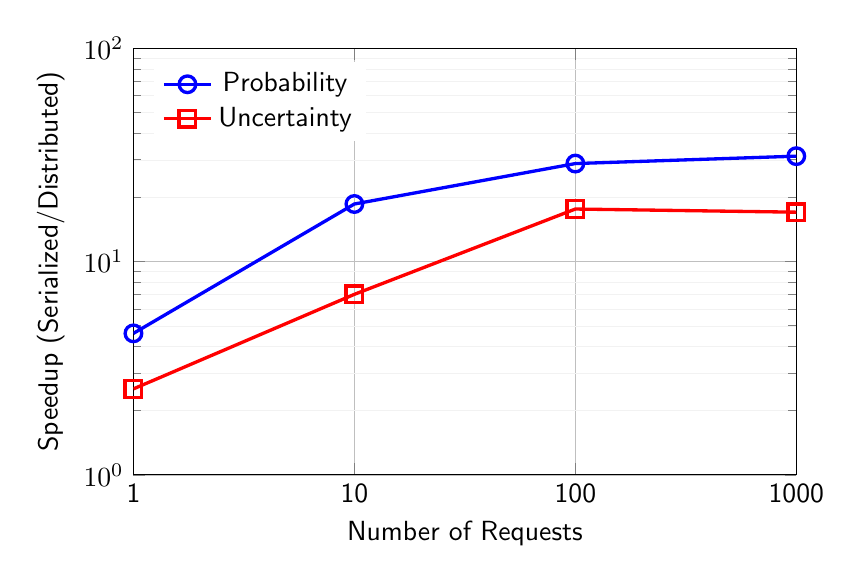
\begin{tikzpicture}
        \begin{loglogaxis}[
            width=10cm,
            height=7cm,
            grid=both,
            minor grid style={line width=.1pt, draw=gray!10},
            major grid style={line width=.2pt, draw=gray!50},
            xlabel={Number of Requests},
            ylabel={Speedup (Serialized/Distributed)},
            legend pos=north west,
            legend style={draw=none},
            xtick={1,10,100,1000},
            xticklabels={1,10,100,1000},
            log basis x=10,
            log basis y=10,
            ymin=1, ymax=100,
            xmin=1, xmax=1000
            ]
            
            % Probability speedup data
            \addplot[
                color=blue,
                mark=o,
                line width=1.2pt,
                mark size=3pt
                ] coordinates {
                (1, 4.603)
                (10, 18.6)
                (100, 28.776)
                (1000, 31.167)
            };
            
            % Uncertainty speedup data
            \addplot[
                color=red,
                mark=square,
                line width=1.2pt,
                mark size=3pt
                ] coordinates {
                (1, 2.528)
                (10, 7.016)
                (100, 17.616)
                (1000, 17.029)
            };
            
            \legend{Probability, Uncertainty}
        \end{loglogaxis}
    \end{tikzpicture}
    \caption{Speedup comparison between serialized and distributed execution for different request volumes.}
    \label{fig:speedup}
\end{figure}

The super-linear speedup for single request workloads is caused by the elimination of I/O processes. In the serialized \texttt{scram-cli} baseline, each run must (i) parse command-line arguments, (ii) read and validate the input XML fault-tree, (iii) launch a new process to execute the solver, and (iv) synchronously write results back to disk. In the distributed implementation, the request payload already contains the model and run-time parameters, which are passed directly to a Node.js native addon that invokes the underlying \texttt{scram} library. Result persistence is off-loaded to an asynchronous database writing process. So, both the initial XML parsing and the final file output are effectively removed from the process. Consequently, execution time reflects only the core solver computation, producing the observed speed-ups ($S\approx4.6$ for probability estimation and $S\approx2.5$ for uncertainty analysis) even at a single concurrent request.  
Beyond 100 jobs, speed-up saturates owing to:

\begin{itemize}
  \item \textbf{Worker saturation}: eight containers fully occupy the host's 8 hardware threads; adding jobs only increases wait time.
  \item \textbf{Queue latency}: larger batches incur longer residence times in RabbitMQ prior to dispatch.
  \item \textbf{Memory bandwidth limits}: uncertainty calculations are memory-bound; waiting time grows with concurrency.
\end{itemize}

These findings validate that the combined architecture of Docker-Swarm and RabbitMQ delivers near-linear scaling for practical PRA workloads up to the tested concurrency and provides an order-of-magnitude reduction in wall-clock time compared with serialized execution.
}

% \section{Handling Multi-Hazard Models in Parallel}
% \subsection{Integration of Hazard Modules}
% \subsection{Numerical Stability and Overflow Handling}

% \section{Security and Data Ownership}
% \subsection{Data Sharing Protocols}
% \subsection{Access Control and Regulatory Constraints}
% \chapter{Task III: Testing and Benchmarking Code Optimizations}
\label{cha:task_iii}


\input{task_III/saphsolve/optimizations}
\input{task_III/saphsolve/postprocessing}


\section{SCRAM Optimizations}

The SCRAM tool underwent a series of targeted optimizations to address both algorithmic and implementation level inefficiencies, with the primary goal of improving runtime performance for large-scale \acrshort{pra} models. The optimizations focused on two main areas: (1) data structure modernization and (2) parallelization of computationally intensive routines.

\paragraph{Data Structure Modernization}

The first set of optimizations involved migrating internal data structures from custom, pointer-based representations to \acrfull{stl} containers. Specifically, \acrshort{zdd} container, which holds minimal cut sets, was refactored to utilize \acrshort{stl} containers. Similarly, containers responsible for storing processed minimal cut sets were also migrated to \acrshort{stl}. This transition was motivated by prior profiling, which indicated that a significant portion of solver time was consumed by postprocessing logic, particularly within the reporter module. By leveraging \acrshort{stl} containers the codebase benefits from improved memory management.
 
\paragraph{Exploiting Parallelism with OpenMP}

The second major optimization involved the introduction of parallelism using OpenMP. Parallelization was applied to several computationally expensive routines, including:

\begin{itemize}
    \item Probability calculation using the \acrshort{mcub} and \acrshort{rea} methods,
    \item Importance analysis, and
    \item Uncertainty quantification.
\end{itemize}

\paragraph{Performance Results and Interpretation}

The computational gains achieved through these optimizations are summarized in the tables that follow. Table~\ref{tab:scram_prob_runtimes_aralia} presents probability calculation runtimes for the three most computationally demanding Aralia models, comparing serial (single-core) and OpenMP-enabled (eight-core) executions. The results show that parallelization of the probability calculation routine yields a speedup of approximately 3$\times$ for the probability computation step, while the overall total runtime speedup is more modest (about 1.04$\times$), indicating that other parts of the workflow remain serial or are less amenable to parallelization.

\input{task_III/scram/tables/scram_prob_runtimes_aralia}

Table~\ref{tab:reporter_improvements} summarizes the effect of data structure modernization and parallelization on the reporter module. Across the ARALIA models, the reporter's runtime is reduced by factors ranging from 1.44$\times$ to over 3.05$\times$, with corresponding overall speed-ups of 1.08$\times$ to 2.42$\times$ in total runtime. Notably, the largest models (e.g., \texttt{edfpa14b}, \texttt{edfpa14o}, \texttt{edfpa14q}) exhibit more pronounced gains than before, showing the benefits of the optimizations.

\input{task_III/scram/tables/scram_reporter_runtimes_aralia}

Table~\ref{tab:runtime_improvement_runs_summary} provides a detailed breakdown of runtimes for importance analysis, uncertainty quantification, and the reporter module, before and after optimization. The results consistently show reductions in execution time across all three categories, with total runtime speedups frequently exceeding 3$\times$ for large models. Table~\ref{tab:improvement_runs_summary} further distills these results into explicit speedup factors, highlighting the performance gains due to the implemented changes.

\input{task_III/scram/tables/scram_all_runtimes_aralia}

Collectively, these results confirm that the combination of data structure modernization and parallelization delivers significant performance improvements for SCRAM, particularly for large and complex PRA models. The observed speedups translate directly into increased throughput and reduced latency for risk quantification tasks, enabling more timely and responsive risk-informed decision-making.

\input{task_III/scram/tables/scram_all_speedups_aralia}

\paragraph{Limitations and Future Work}

Despite these advances, certain limitations remain. The \acrshort{bdd} method still uses a custom data structure, and \acrshort{bdd}-based probability calculations are performed serially. This represents a bottleneck for models that rely heavily on \acrshort{bdd} representations. Future work should explore the integration of multi-core and GPU-accelerated \acrshort{bdd} solvers, which have the potential to reduce computation times and improve scalability for even larger models.

{
\cleardoublepage
\let\clearpage\relax
\include{4_proposed_solution/overview/_}

\chapter{Designing a Distributed Queuing System}

\section{Worker-Pool and Queue Management Concepts}

The distributed system follows a \emph{publisher--consumer} pattern. In this architecture, a \textbf{publisher} is typically a client-facing service, such as REST \acrshort{api}s, responsible for receiving requests from front-end clients and forwarding these requests to an exchange inside a message broker. A \textbf{message broker} is a middleware system that facilitates communication between publishers and consumers by routing messages.

Within the broker, the \textbf{exchange} component directs each request to an appropriate queue based on the routing key of the request. A \textbf{queue} is a data structure within the broker that temporarily stores messages until they are processed by consumers. Each queue is configured with specific user-defined settings, such as message time-to-live, maximum queue length, and prefetch limits (the maximum number of messages that a consumer can process simultaneously).

A \textbf{scheduler} layer adds service-level metadata to these messages, including priority, delays, and enforces ordering policies such as \acrshort{fifo} or strict priority ordering. \acrshort{fifo} ensures that messages are processed in the order they arrive, while strict priority ordering processes messages based on assigned priority levels. Queues can be marked as durable, enabling recovery of messages in case of broker restarts or failures. Messages can be marked as persistent, guaranteeing delivery despite network or consumer disruptions. Additionally, queues support a \textbf{dead-letter queue} mechanism, a specialized queue that captures undeliverable or failed messages, allowing for subsequent analysis and recovery operations.

A \textbf{consumer} represents any \acrshort{pra} solver instance within the worker pool. The \textbf{worker pool} is essentially a collection of solver processes running on \acrshort{cpu}s, \acrshort{gpu}s, or \acrshort{fpga}s. These consumers connect to their designated queues and consume messages based on prefetch settings. Consumers process each message by retrieving the \acrshort{pra} models and solver parameters from the message body. Then they perform calculations and persist the results in the distributed databases. Upon successful completion, they send an \textbf{acknowledgement}, a confirmation message indicating successful processing, back to the broker, marking the message as processed.

The broker implements idempotent operations, meaning duplicate or repeated actions are processed only once. For example, if the user repeatedly attempts to create a queue, the broker will create the queue once and ignore the rest of the repeated commands. Finally, both publishers and consumers send periodic heartbeats, regular signals or pings, to the broker to ensure the active status of these components. These heartbeats allow the developers to monitor service availability and manage the health of the distributed system. Figure \ref{fig:worker-pool-queue-management} shows a basic publisher-consumer workflow of a message broker.

\input{4_proposed_solution/dist_queues/plots/plot_dist_msg_broker}

\section{REST APIs for Parallel Task Coordination}

The platform provides a RESTful \acrshort{api} layer that orchestrates the entire life cycle of \acrshort{pra} quantification tasks, from submission and monitoring to cancellation and result retrieval. An \acrshort{api} is a set of rules that lets different software systems exchange data programmatically over the internet. A RESTful \acrshort{api} implements these rules using standard \acrshort{http} methods (GET, POST, PUT, DELETE) and resource-oriented \acrshort{url}s to ensure stateless communication. The REST \acrshort{api}s handles client authentication and payload validation, translating task definitions (\acrshort{pra} models and solver parameters) into messages dispatched to the publisher component of the distributed system. Upon successful POST, clients receive a unique task identifier, which they use to subscribe to status endpoints to get real-time execution updates (queued, running, completed, failed). Batch submission endpoints accept arrays of quantification tasks with optional metadata for target solver selection (\acrshort{mocus}/\acrshort{bdd}/\acrshort{zdd}/Monte Carlo), priority levels, and estimated resource requirements. Result endpoints expose completed outputs and solver performance metrics in \acrshort{json} format via secure download \acrshort{url}s pointing to the distributed databases. To ensure fair usage, the \acrshort{api}s implement idempotent POST semantics and rate limiting to prevent duplicate requests and resource starvation. Figure \ref{fig:rest-api-architecture} shows a simplified workflow of the REST API layer.

\input{4_proposed_solution/dist_queues/plots/plot_dist_rest_api}

\section{Design of the Distributed System}

\subsection{Load Balancing and Scheduling}

The distributed architecture is designed to handle a high volume of concurrent PRA quantification tasks with minimal latency and maximum resource utilization. To achieve this, the system employs containerization and cluster orchestration to distribute workloads across multiple computing nodes, combined with scheduling policies to balance the load. Quantification jobs are managed through a message-queue system that decouples task submission from execution, enabling tasks to be executed in parallel by a pool of workers. The framework statically scales the number of worker instances before launch and assigns each job type to its own queue. This scheduling approach reserves resources for every class of quantification task and enables rapid deployment of additional workers when larger models--or large-scale studies--must be processed. Core strategies include (i) distributing tasks across dedicated queues in a Docker Swarm cluster, (ii) using a multi-queue workload manager, (iii) partitioning complex models into parallel tasks, and (iv) adaptively selecting algorithms for each stage of the analysis. These measures collectively provide efficient load balancing and scheduling for the platform's quantification engine.

\subsection{Distributed Task Scheduling in the Cluster}

The distributed queuing system is structured as two loosely coupled, independently deployable microservices within a mono repository: one implements the publisher service, and the other implements the consumer service. These microservices are then deployed as Docker services across a Docker swarm cluster \cite{Swarm}. The cluster consists of a manager node and multiple worker nodes. The manager node is responsible for orchestrating operations and maintaining the cluster state (e.g., monitoring node health and resource usage), while the workers execute the quantification tasks. Both the backend producer service and the worker (consumer) service are containerized as separate Docker  images. The producer service (running on one or more instances) handles incoming analysis requests. It runs the NestJS-based backend \cite{Documentation} and connects to RabbitMQ \cite{RabbitMQ} and the MongoDB \cite{MongoDB} database, and the worker service encapsulates the scram \cite{scram} quantification engine via its Node.js NAPI \cite{Node} bindings, along with its own RabbitMQ client and database access.

When a user submits a model for quantification (for example, by clicking “Quantify” in the web editor or via a REST API call), an HTTP request with the model data and analysis parameters is sent to the backend (producer) service. To avoid sending large files over the network or through the message queue, the backend stores the model input (OpenPSA MEF XML files \cite{2017OpenPSAMEF}) in the MongoDB database and retains only a document ID. The request is then tagged with metadata including the document ID and the requested analysis type. At this point, a priority level is assigned based on the analysis type or urgency of the task. For instance, a simple point estimate might be treated as high priority, whereas a lengthy uncertainty propagation could be set as lower priority. The producer then serializes the task description including the document ID and priority into a message and enqueues it into a RabbitMQ job queue. RabbitMQ serves as the central task broker -- it enables asynchronous handling of potentially thousands of jobs without overloading the web server, and it routes tasks to available workers. If multiple producer instances are running, a Traefik \cite{Traefik} load balancer distributes incoming HTTP requests among them, preventing any single backend instance from becoming a bottleneck and thereby balancing the load at the entry point of the system.

On the execution side, a fleet of worker containers run on the Swarm cluster's worker nodes to perform the actual model quantifications. The manager node can scale the number of active worker containers up or down (currently up to 128 workers across the cluster) to match the incoming workload demand. Each worker continuously polls the RabbitMQ queue for new jobs. RabbitMQ supports multiple queues, so jobs can be segregated by priority or type, and the workers always draw the highest priority jobs first from their individual queues. Once a worker retrieves a job message, it fetches the corresponding model input data from MongoDB (using the document ID in the message), then invokes the scram engine via the Node.js native addon to perform the quantification. By containerizing the scram engine and associated libraries, the system isolates each task's execution while allowing it to fully utilize a CPU core (or multiple cores if the engine itself is multi-threaded) on the worker node. After the quantification completes, the worker saves the output (results files, logs, etc.) back to the database, associating them with the same document ID for later retrieval. It then sends an acknowledgment to RabbitMQ so that the message is removed from the queue. The platform uses RabbitMQ's manual acknowledgment mechanism: a task message is only cleared from the queue when a worker signals successful completion. If a worker crashes or fails before finishing, the lack of acknowledgment causes RabbitMQ to automatically re-queue the task, making it available for another worker to pick up. \emph{Figure~\ref{fig:distributed-workflow}} illustrates this distributed workflow: multiple producers accept user requests and queue tasks, and a pool of workers on the cluster consume tasks, quantify and return results.

\input{4_proposed_solution/dist_queues/plots/plot_dist_workflow}

\subsection{Multi-Queue Workload Management}
\label{subsec:multi-queue}

The system currently employs a multi-queue architecture that routes requests according to solver execution mode. The worker replicas are statically scaled up (or down), so the cluster cannot dynamically reallocate computational resources among queues. Hence, priority-based routing is not available. Only intra-queue priorities are ensured, meaning higher-priority messages within a queue are processed before lower-priority ones. All queues are hosted in the same RabbitMQ broker, but each provides messages to a distinct worker deployment and calls a different execution pathway inside the cluster.

\paragraph{Queue type~1: API--Model jobs}
This type of queue is used when a client sends an \textsc{http} \texttt{POST} request to \texttt{/quantify} endpoint. The request contains the PRA model in Base64 form (the payload is an OpenPSA MEF XML file, converted to a single Base64 string) together with the chosen solver name (\texttt{scram-bdd}, \texttt{scram-mocus}, \texttt{scram-mc} etc.) and any run parameters. The producer service stores the raw model in MongoDB, inserts the \texttt{model id} along with solver parameters into a JSON task document, and publishes that document to the queue.  A pool of \texttt{model worker} containers subscribes exclusively to this queue.

Each worker:

\begin{enumerate}
  \item Retrieves the task, downloads the model blob from MongoDB, and
        writes it to a temporary file inside the container.
  \item Invokes the designated solver on that file.
  \item Persists the results back to the database and acknowledges the message.
\end{enumerate}

Since the model travels with the message, these jobs are fully self-contained and the cluster does not require shared storage.

\paragraph{Queue~2: API--Exec jobs}
When the client prefers not to embed the PRA model in the request payload, the solver can be invoked as a shell command within a working directory that already contains the input files. In this case, the client sends an HTTP \texttt{POST} request to the \texttt{/execute} endpoint that specifies:

\begin{itemize}
  \item \texttt{workdir} -- the absolute path visible on the cluster where the model files reside.
  \item \texttt{cmdline} -- the exact tool invocation, identical to how the user would call it on a login node (e.g.\
  \verb|scram --mocus --mcub ft-310.xml|).
\end{itemize}

The producer wraps these two strings in a task document and publishes it
to the queue. A separate deployment of \texttt{exec worker} containers subscribes to this queue; each worker simply change directories into \texttt{workdir} and executes the given command under a limited access shell. This design keeps large input datasets out of the message queues and databases.

\subsection{Model Partitioning for Parallel Execution}

In addition to managing discrete jobs, the quantification engine employs model-specific partitioning strategies to leverage parallelism within a single large analysis. Complex PRA models -- notably, large event trees with many branching sequences or scenarios that each depend on fault tree evaluations -- are broken down into smaller sub-tasks that can be solved concurrently. Rather than treating a monolithic model as one giant quantification problem, the system identifies independent submodels (subtrees of the overall logic) and distributes those as separate jobs to the cluster. For example, consider an event tree analysis that involves hundreds of linked fault trees (one fault tree for each sequence or safety function outcome). Instead of quantifying each sequence serially, the platform treats each fault tree as an independent quantification task. All fault trees can then be processed in parallel across the distributed workers, each producing a failure probability or cut set result for its respective portion of the event tree. Once all these parallel computations are complete, a post-processing step aggregates the results: the event tree logic is applied to combine the sequence-level probabilities (or other metrics) into an overall result, which is then reported to the user as a single coherent output. This divide-and-conquer strategy acts as a pre-processing (decomposition) and post-processing (recomposition) workflow that enables the handling of extremely complex models which would be infeasible to solve in a single thread or single process. By performing dozens or hundreds of sub-calculations simultaneously, the system can significantly reduce the wall-clock time for quantifying large-scale PRA models.

One advantage of this partitioned approach is that the user can obtain interim results or a rough overview quickly, even if the full analysis is intricate. Because the most critical sub-tasks can be prioritized or because partial results become available as sub-tasks finish, the system could provide a preliminary risk estimate after the first wave of subtrees is solved, then refine that estimate as the remaining subtrees complete. In practice, the initial results might be less precise (for instance, based on a subset of scenarios or a simplified combination of outcomes), but as more computational resources come online or as more sub-tasks finish, the overall result converges to the high-accuracy answer. This means the platform can deliver a quick assessment to analysts (useful for time-sensitive decision support) and then follow up with increasingly accurate results as computation continues, effectively trading off accuracy and time. 

Moreover, the engine takes an adaptive algorithmic approach during quantification to optimize both accuracy and performance for each sub-task. Different solving algorithms excel under different conditions, so the engine can choose the most appropriate method on a per-subtask basis. For example, the MOCUS algorithm (which enumerates minimal cut sets) is very fast for low-probability scenarios but tends to lose accuracy (overestimating the top event probability) in scenarios with high component failure probabilities, due to the limitations of the rare-event approximation. On the other hand, binary decision diagram (BDD) based methods yield exact results even with higher failure probabilities but can be slower or more memory-intensive for very large logic structures. To capitalize on these strengths, the system can automatically apply a BDD-based quantification for portions of the model that involve high probability events or densely interdependent logic, while using MOCUS (potentially with approximations like the min-cut upper bound, MCUB) for other portions. In the previous example of an event tree with many fault trees, this might mean using a BDD solver for a particular fault tree known to have high-risk (high probability) contributors, and using the faster cut-set solver for fault trees in which the rare-event assumption holds. By mixing algorithms in this way, each sub-task is solved with the method best suited to its characteristics, ensuring that the final results are accurate without incurring unnecessary computational overhead.

\subsection{Handling Shared Subtrees in Distributed Memory} A particular challenge in the parallel decomposition of a PRA model is handling shared subtrees in a distributed memory environment. Shared subtrees occur when different parts of a model require the evaluation of an identical sub-model. For instance, in an event tree analysis, multiple accident sequences might involve the same mitigating system fault tree; similarly, in a large fault tree, two separate top events or portions of the logic might include a common subtree (a repeated gate structure or module). In a single-process solver, such common substructures can be computed once and reused internally to save time. However, in a distributed system each worker operates with its own memory and state, so without coordination, the same subtree could be sent to two different workers and thus be quantified twice in isolation. This would waste computational effort. The scheduling strategy avoids this by ensuring that each unique subtree is solved only once.

Before distributing tasks, the system identifies any duplicate or shared subtrees among the jobs. Rather than dispatching redundant tasks, it will assign the computation of a shared subtree to a single designated worker and hold or coordinate the dependent tasks until that worker produces the result. For example, if two event tree sequences both require the fault tree FT1, the scheduler will create a task for quantifying FT1 only once. The first sequence that needs FT1 triggers the FT1 task to be queued; the second sequence's task sees that FT1 is already in progress (or completed) and will not generate a duplicate FT1 job. When the one worker finishes solving FT1, its results (cut sets, intermediate BDD, or failure probability) are stored in a common repository -- in this case, the MongoDB database -- and indexed by an identifier (such as the subtree's ID). Then, any pending computations that depend on that subtree can retrieve the result and proceed without recomputing it.

In the event tree scenario, once fault tree FT1's probability is known, it can be plugged into all sequences that require it, and those sequences' quantifications can continue or be finalized. This mechanism effectively simulates a shared memory for that piece of data: although the cluster is distributed, the intermediate result is made available to all relevant processes through the centralized database. During the aggregation phase, the coordinator (a processed job service dedicated for aggregation process) combines the unique results from each subtree to form the overall outcome. This approach does require careful scheduling logic -- workers might need to wait for a shared dependency to be solved by another worker. This implementation is essential for large PRA models, where repeated subtrees are prevalent.

\section{Implementation of the Distributed System}

\subsection{Software Stack and Technology Selection}

\textbf{NestJS, TypeScript and RabbitMQ:} The platform uses NestJS, a Node.js based framework, with TypeScript \cite{starting} for its web services. TypeScript's static typing reduces runtime errors by validating the request and response payloads at compile time. NestJS provides a modular architecture with dependency injection and out-of-the-box support for microservices that simplifies building structured REST API based services. RabbitMQ provides all the advanced features of a message broker at no cost, while ensuring high-throughput and low latency for job processing.

\textbf{MongoDB:} Distributed MongoDB databases are used for persisting PRA models and results. MongoDB was selected for its flexible document schema and horizontal scalability (via sharding). This schema flexibility is ideal for PRA data (e.g., fault trees, event trees, Bayesian networks, etc.) which can have heterogeneous structures.

\textbf{C++ Quantification Engine (scram) and NAPI:} The quantification tasks are handled by the scram engine, written in C++. To integrate this native engine with the TypeScript language, OpenPRA employs Node's N-API (Node Addon API). N-API bridges the TypeScript and C++ layers by compiling scram's functions into a Node.js module, allowing the TypeScript code to invoke C++ quantification methods directly. This approach offers the speed of optimized C++ code while keeping the high-level logic in TypeScript, and abstracts away the complexity of the C++ codebase from the rest of the system.

\textbf{OpenMP for Multi-core Parallelism:} Within the scram engine, OpenMP is utilized to parallelize computations across multiple CPU cores. Certain analyses (e.g. uncertainty and importance measure) run in parallel threads.

\textbf{GPU Acceleration (CUDA/SYCL):} The platform also explores GPU computing to accelerate PRA analysis. Using C++ heterogeneous computing frameworks like SYCL \cite{Alpay2020SYCL}, which can target NVIDIA CUDA GPUs or other accelerators, it has been demonstrated that offloading Monte Carlo simulations to a GPU can drastically reduce computation time. Such GPU integration is considered for high-priority or large-scale simulations to further enhance throughput.

\subsection{Containerization/Virtualization Strategies}

The publisher service and the consumer service are each packaged as separate Docker container images. Docker is a widely adopted container platform that provides portable, consistent execution environments with minimal overhead. In high-performance computing environments where administrative privileges are restricted, Singularity can be utilized as an alternative container runtime. Containers share the host kernel, offering low resource usage. Docker Swarm, a container orchestration tool, manages the deployment of these containers across multiple nodes. The manager node schedules services and maintains cluster states. A Traefik load balancer distributes incoming REST \acrshort{api} requests evenly among publisher instances. Dedicated computing nodes are connected by high-speed interconnects (such as high-speed Ethernet) ensuring low-latency communications.

Resource allocation and management are orchestrated through a declarative configuration defined in a Docker Compose file, which specifies service deployment, network connectivity, resource constraints, and scaling policies.

Each service, including frontend interfaces, backend \acrshort{api} endpoints, job brokers, and computation workers, is deployed as a containerized application with explicit resource management policies.

\begin{itemize}
    \item \textbf{Dynamic scaling:} Services such as \texttt{job-publisher} are dynamically scaled using Docker Swarm's replicated deployment mode. This service is set up with adjustable replication factors (up to 128 replicas per node).
    
    \item \textbf{Placement constraints:} Placement constraints, defined via node labels (e.g., \texttt{host\_performance}), restrict deployment to specific nodes according to computational requirements. Resource-intensive services like \texttt{mongodb} and \texttt{rabbitmq} are constrained to nodes labeled for high performance.
    
    \item \textbf{Load balancing and scheduling:} Traefik serves as the primary load balancer, routing incoming \acrshort{http} and \acrshort{https} requests among service replicas based on predefined routing rules. Each microservice (frontend, backend, and job brokers) is configured with constraints such as \texttt{max\_replicas\_per\_node}, ensuring balanced distribution of containers across available nodes and avoiding single-node overload.
    
    \item \textbf{Update and rollback management:} Services share a unified update and rollback configuration. Updates are executed in parallel (up to 16 instances simultaneously), with rollback mechanisms triggered upon failure.
    
    \item \textbf{Resource isolation and limits:} Explicit CPU and memory constraints can be configured in the Docker Compose file to prevent resource exhaustion.
    
    \item \textbf{Health Monitoring:} Health checks are systematically performed on each service instance, using predefined intervals and thresholds to detect unhealthy containers quickly. Unresponsive or failing containers are automatically restarted.
\end{itemize}

\input{4_proposed_solution/dist_queues/deployment}

\section{Performance Evaluation and Scaling Results}
\label{sec:scaling-results}

\subsection{Experimental Setup}
\label{subsec:exp-setup}

Benchmark tests were executed on a workstation equipped with a 13\textsuperscript{th}-Gen Intel\textsuperscript{\textregistered} Core\textsuperscript{\texttrademark} i7-13700K (16 cores, 24 threads) and 32 GB RAM. Deploying the distributed system on an entry-level CPU and a single node was intentional: it demonstrates that the distributed system can run on off-the-shelf hardware without setting up a specialised network or cluster-management expertise. With fewer cores, performance-scaling plateaus appear sooner than they would on a large cluster, allowing bottlenecks to be identified earlier in the development cycle.

The \textit{baobab3.xml} fault-tree model from the Aralia fault tree data set served as the workload. Two scenarios were compared:

\begin{enumerate}
  \item \textbf{Serialized baseline:} direct invocation of \texttt{scram-cli} (single process, no queue).
  \item \textbf{Distributed system:} eight Dockerised worker containers orchestrated by Docker swarm, with jobs submitted through the REST \acrshort{api} and routed via RabbitMQ.
\end{enumerate}

End-to-end latency was measured from \textsc{http} \texttt{POST} reception to result retrieval for batches of 1, 10, 100, and 1000 concurrent requests. Two task types were profiled: point-estimate probability calculation and uncertainty quantification.

\subsection{Results and Discussion}
\label{subsec:scaling-discussion}

Table~\ref{tab:benchmark-times} lists the mean execution times (\SI{}{\second}) over four runs per workload.  
Speed-up $S$ is defined as
\input{4_proposed_solution/dist_queues/equations/eq_dist_speedup}

\input{4_proposed_solution/dist_queues/tables/table_dist_q_exec_times}

Figure~\ref{fig:speedup} depicts the resulting speed-up.  
For probability calculations the system scaled almost linearly up to 100 simultaneous jobs, peaking at $S\approx31$ for 1000 requests before reaching a plateau.  
Uncertainty quantification, which is more compute-intensive, achieved $S\approx18$ at 100 jobs, after which the speedup slightly decreased.

\input{4_proposed_solution/dist_queues/plots/plot_dist_q_speedup}

The super-linear speedup for single request workloads is caused by the elimination of I/O processes. In the serialized \texttt{scram-cli} baseline, each run must (i) parse command-line arguments, (ii) read and validate the input XML fault-tree, (iii) launch a new process to execute the solver, and (iv) synchronously write results back to disk. In the distributed implementation, the request payload already contains the model and run-time parameters, which are passed directly to a Node.js native addon that invokes the underlying \texttt{scram} library. Result persistence is off-loaded to an asynchronous database writing process. So, both the initial XML parsing and the final file output are effectively removed from the process. Consequently, execution time reflects only the core solver computation, producing the observed speed-ups ($S\approx4.6$ for probability estimation and $S\approx2.5$ for uncertainty analysis) even at a single concurrent request.  
Beyond 100 jobs, speed-up saturates owing to:

\begin{itemize}
  \item \textbf{Worker saturation}: eight containers fully occupy the host's 8 hardware threads; adding jobs only increases wait time.
  \item \textbf{Queue latency}: larger batches incur longer residence times in RabbitMQ prior to dispatch.
  \item \textbf{Memory bandwidth limits}: uncertainty calculations are memory-bound; waiting time grows with concurrency.
\end{itemize}

These findings validate that the combined architecture of Docker-Swarm and RabbitMQ delivers near-linear scaling for practical PRA workloads up to the tested concurrency and provides an order-of-magnitude reduction in wall-clock time compared with serialized execution.
}

% \section{Handling Multi-Hazard Models in Parallel}
% \subsection{Integration of Hazard Modules}
% \subsection{Numerical Stability and Overflow Handling}

% \section{Security and Data Ownership}
% \subsection{Data Sharing Protocols}
% \subsection{Access Control and Regulatory Constraints}
%{
\cleardoublepage
\let\clearpage\relax
\section*{High-Level System Components}

The proposed \acrshort{hpc} architecture leverages three distinct computational strategies to improve the speed, efficiency, and throughput of \acrshort{pra} quantifications. These approaches address the computational demands of modern \acrshort{pra} by utilizing available hardware resources and parallel computation techniques.

\begin{enumerate}

    \item \textbf{Parallel Computation on Shared Memory:} Implemented primarily for importance measures and uncertainty quantification tasks, this approach utilizes multicore \acrshort{cpu} architectures (e.g., via \acrshort{openmp}) to parallelize computations.
    
    \item \textbf{Task-Parallel Distributed System on Distributed Memory:} This implementation is designed to horizontally scale \acrshort{pra} solvers. Computational tasks including probability estimation, uncertainty analysis, and importance measures are assigned as discrete tasks to independent computational nodes. Tasks are managed via REST \acrshort{api}s interfacing with a distributed task queue, facilitating concurrent task execution.
    
    \item \textbf{Data-Parallel Monte Carlo Probability Estimator:} Specifically developed for probability estimation, this solver turns fault trees into layered graphs that can be simulated in parallel on \acrshort{gpu}s or multicore \acrshort{cpu}s. Millions of random samples of each basic event are generated and bit-packed to reduce memory usage. \acrshort{sycl} kernels then work their way up the layers, combining the results in topological order and use hardware-accelerated pop-count instructions to evaluate the outcome of the gates on the fly.
\end{enumerate}

Collectively, these strategies enable the modernized \acrshort{pra} platform to handle much larger models, compute them faster, and process many more concurrent quantifications than was previously possible.

% \subsection{Priority Queues and Active Queue Management Strategies}\label{subsec:priority-aqm}

% \subsection{GPU Acceleration and CPU-Multicore Approaches}\label{subsec:gpu-accel}

% \section{A Brief History of PRA Tools}
% \label{sec:history_of_pra_tools}

% Probabilistic Risk Assessment (PRA) has evolved dramatically since its inception in the 1970s, driven both by the growing complexity of nuclear power systems and by substantial leaps in computing technology. Early PRA efforts were primarily focused on relatively small reactor models, typically analyzed with mainframe computers or custom in-house codes. Over time, the field has shifted from batch-oriented, single-CPU environments to desktop-based tools and, more recently, to parallel and cloud-based software poised to exploit high-performance computing (HPC). This section first outlines the motivations for PRA software over the decades and then examines representative PRA tools, culminating in a contemporary view of how evolving hardware, licensing, and operational needs have given rise to the current landscape.

% \subsection{Computing Landscape from the 1970s to the 2020s}

% \paragraph{1970s: Mainframe Computing and Foundational PRA Studies.}
% The seminal Reactor Safety Study (WASH-1400) in the mid-1970s introduced wide-ranging probabilistic techniques for assessing reactor safety. While this study provided a rigorous framework, it also underscored the limitations imposed by mainframe computing resources, which constrained the size of fault trees and event trees that could be analyzed. Early PRA codes, such as PREP and KITT~\cite{vesely_prep_1970,vesely_prep_1997}, operated in these mainframe environments and performed either Monte Carlo or deterministic methods to identify Minimal Cut Sets (MCS) and compute their probabilities.

% \paragraph{1980s--1990s: Transition to Personal Computers.}
% By the 1980s, the expansion of Light Water Reactor (LWR) licensing and the increasing complexity of PRA models led to the introduction of more advanced tools. MOCUS~\cite{Fussell1974MOCUS}, MODULE~\cite{module}, SIGPI~\cite{sigpi}, and RISKMAN~\cite{riskman1,riskman2} are examples of software developed to handle larger fault trees and event trees, shifting computational tasks onto personal computers rather than mainframes. While personal computers substantially reduced hardware costs, early desktop-based PRA tools often suffered from limited memory, slower processors, and rudimentary user interfaces. Nevertheless, this period saw the gradual shift toward stand-alone, desktop-centric PRA applications that offered more intuitive workflows.

% \paragraph{2000s: Emergence of Distributed, Web-Based, and Parallel Solutions.}
% With improving desktop performance and the emergence of web-based applications, more collaborative PRA tools began to appear. At the same time, parallel computing gained traction, particularly within the broader high-performance computing community. In the PRA world, large-scale event tree and fault tree evaluations were beginning to see benefits from multi-core processors and basic clustering. Tools such as SAPHIRE~\cite{saphire1,SAPHIRE,saphire_manual} (stemming from IRRAS~\cite{irras1,irras2}) expanded the usability of PRA for day-to-day licensing work, while CAFTA~\cite{cafta1,cafta2} and RiskSpectrum~\cite{riskspectrum1} catered to utility operators requiring detailed station-specific reliability calculations. While initial HPC-oriented attempts remained limited, the growing push toward distributed architectures signaled the community's recognition that next-generation PRA problems would benefit greatly from parallel computing paradigms.

% \paragraph{2010s--2020s: Contemporary Large-Scale and GPU-Enabled Paradigms.}
% Continued growth in model complexity--driven by non-LWR reactor designs, multi-hazard considerations, and real-time or near-real-time decision-support needs--further accelerated interest in HPC. During this period, open-source initiatives like SCRAM~\cite{scram} demonstrated how community-driven development could incorporate modern software practices: flexible input formats, automated build pipelines, and expansions for parallel or GPU-based computations. Commercial software packages, including FTREX~\cite{ftrex_manual}, RiskSpectrum, and others, have likewise adapted to multi-core, cluster, and cloud environments, though often in a closed-source manner. Additionally, specialized research frameworks, such as DeRisk~\cite{derisk1,derisk2}, Trilith~\cite{hcl_method}, and HCLA~\cite{hcla_cmd,hcla_web}, illustrate the quest for dynamic or "on-the-fly" risk calculations that can leverage large compute infrastructures.

% \paragraph{Future Trends: Quantum and Fully Homomorphic Encryption.}
% Looking ahead, the community's interest in real-time risk monitoring, coupled with confidentiality requirements for sensitive nuclear data, suggests that quantum computing and fully homomorphic encryption (FHE) could eventually play a role in PRA. Although these technologies remain at a relatively early research stage, their potential for massively parallel or secure distributed calculations could address future bottlenecks in handling multi-hazard complexities, intricate dependencies, or large multi-reactor sites.

% \subsection{Representative PRA Tools and Their Evolution}

% Over the decades, a multitude of PRA software tools have been created and refined, each representing an effort to address the specific computational and regulatory challenges of its time. Table~\ref{tab:pra_tools_overview} summarizes both legacy and contemporary tools, highlighting their licensing models and typical usage contexts. For example, CAFTA~\cite{cafta1,cafta2}, originally designed for DOS-based personal computers, now integrates with advanced Windows environments. SAPHIRE, supported by the U.S. Nuclear Regulatory Commission (NRC) and maintained by Idaho National Laboratory, evolved from earlier codes (IRRAS~\cite{irras1,irras2}), bridging desktop-based analysis and more recent cloud-deployment patterns.

% Even with the proliferation of PRA tools, many remain proprietary, limiting the community's ability to incorporate specialized HPC features or novel algorithms. However, the open-source SCRAM~\cite{scram} suite under the GNU GPL and the MIT-licensed OpenPRA initiative mark a shift toward more collaborative development. These open frameworks foster deeper experimentation with parallel algorithms, advanced sampling methods, and dynamic event-tree evaluations--capabilities that can be critical when analyzing complex, multi-hazard scenarios. Through ongoing cross-institutional collaborations, new HPC extensions are regularly introduced, providing the PRA community with means to surmount performance bottlenecks and scale up to multi-million component analyses.

% \subsection{Opportunities and Limitations in Existing Software}

% Despite considerable efforts to modernize PRA tools, a number of core limitations persist:
% \begin{itemize}
% \item \textbf{Limited Parallelization:} Many legacy applications rely on serial or coarse-grained parallel workflows, insufficient for massive concurrency needs.
% \item \textbf{Closed-Source Development:} Proprietary tools restrict user-driven feature enhancements or specialized HPC adaptations, limiting the scope for research innovation.
% \item \textbf{Platform Dependence:} A heavy focus on Windows-based desktop environments can hamper the integration of containerization, cluster-based scheduling, or cloud-native solutions.
% \item \textbf{Model Size Constraints:} Traditional data structures and memory usage patterns, designed for simpler fault trees and event trees, sometimes struggle with multi-hazard, large-scale models that require efficient parallel memory handling.
% \end{itemize}

% Nonetheless, the increasing availability of cloud resources, multi-node clusters, and GPU-accelerated libraries provides fertile ground for next-generation PRA solutions. By embracing these computational frameworks, practitioners can drastically reduce run times for time-sensitive applications, execute large-scale Monte Carlo or dynamic event-tree analyses, and more readily accommodate expansions into multi-hazard or real-time risk monitoring. This synergy between PRA tools and HPC technologies represents a vital frontier for modeling, regulatory oversight, and operational decision support.

% \subsection{Concluding Remarks on Historical Context}

% From the 1970s mainframe era to modern cloud and GPU-enabled paradigms, PRA software has mirrored the evolution of computing technology. Early codes focused on basic MCS extraction and probability evaluation, while current efforts aspire to large-scale, distributed, and fast-turnaround solutions. This trajectory underscores both the promise and the challenges in harnessing HPC for nuclear risk analysis. The subsequent sections will build upon this historical background, highlighting specific gaps in existing software (Section~\ref{sec:gaps_in_existing_software}) and detailing how contemporary developments in parallel architecture, load balancing, and data management can lead to more robust, accurate, and scalable PRA platforms.


\chapter{Designing a Distributed Queuing System}

\section{Worker-Pool and Queue Management Concepts}

The distributed system follows a \emph{publisher--consumer} pattern. In this architecture, a \textbf{publisher} is typically a client-facing service, such as REST \acrshort{api}s, responsible for receiving requests from front-end clients and forwarding these requests to an exchange inside a message broker. A \textbf{message broker} is a middleware system that facilitates communication between publishers and consumers by routing messages.

Within the broker, the \textbf{exchange} component directs each request to an appropriate queue based on the routing key of the request. A \textbf{queue} is a data structure within the broker that temporarily stores messages until they are processed by consumers. Each queue is configured with specific user-defined settings, such as message time-to-live, maximum queue length, and prefetch limits (the maximum number of messages that a consumer can process simultaneously).

A \textbf{scheduler} layer adds service-level metadata to these messages, including priority, delays, and enforces ordering policies such as \acrshort{fifo} or strict priority ordering. \acrshort{fifo} ensures that messages are processed in the order they arrive, while strict priority ordering processes messages based on assigned priority levels. Queues can be marked as durable, enabling recovery of messages in case of broker restarts or failures. Messages can be marked as persistent, guaranteeing delivery despite network or consumer disruptions. Additionally, queues support a \textbf{dead-letter queue} mechanism, a specialized queue that captures undeliverable or failed messages, allowing for subsequent analysis and recovery operations.

A \textbf{consumer} represents any \acrshort{pra} solver instance within the worker pool. The \textbf{worker pool} is essentially a collection of solver processes running on \acrshort{cpu}s, \acrshort{gpu}s, or \acrshort{fpga}s. These consumers connect to their designated queues and consume messages based on prefetch settings. Consumers process each message by retrieving the \acrshort{pra} models and solver parameters from the message body. Then they perform calculations and persist the results in the distributed databases. Upon successful completion, they send an \textbf{acknowledgement}, a confirmation message indicating successful processing, back to the broker, marking the message as processed.

The broker implements idempotent operations, meaning duplicate or repeated actions are processed only once. For example, if the user repeatedly attempts to create a queue, the broker will create the queue once and ignore the rest of the repeated commands. Finally, both publishers and consumers send periodic heartbeats, regular signals or pings, to the broker to ensure the active status of these components. These heartbeats allow the developers to monitor service availability and manage the health of the distributed system. Figure \ref{fig:worker-pool-queue-management} shows a basic publisher-consumer workflow of a message broker.

\begin{figure}[h]
  \centering
  \begin{tikzpicture}[
      scale=0.7,
      >=stealth,
      box/.style={draw,rectangle,minimum width=2cm,
                  minimum height=0.8cm,align=center},
      msg/.style={->, thick},
      label/.style={font=\small,draw=none}
    ]
    
    % Message Broker components
    \node[box] (exchange) {Exchange};
    \node[box, right=1.5cm of exchange] (queue) {Queue};
    \node[box, below=0.8cm of queue] (dlq) {Dead-Letter\\Queue};
    
    % Fit node for RabbitMQ Message Broker
    \node[fit=(exchange)(queue)(dlq),
          draw, inner sep=0.3cm, dashed, 
          label={[yshift=0.3cm]\textbf{RabbitMQ}}] (broker) {};
    
    % Publisher and Consumer
    \node[box, left=2cm of exchange] (publisher) {Publisher};
    \node[box, right=1.5cm of queue] (consumer) {Consumer\\(PRA Solver)};
    
    % Draw connections
    \draw[msg] (publisher) -- node[above,label]{requests} (exchange);
    \draw[msg] (exchange) -- node[above,label]{routing} (queue);
    \draw[msg] (queue) -- node[above,label]{deliver} (consumer);
    
    % Failed messages
    \draw[msg] (exchange) |- node[pos=0.25,left,label]{failed} (dlq);
    
  \end{tikzpicture}
  \caption{Publisher-consumer message flow with broker internals.}
  \label{fig:worker-pool-queue-management}
\end{figure}

\section{REST APIs for Parallel Task Coordination}

The platform provides a RESTful \acrshort{api} layer that orchestrates the entire life cycle of \acrshort{pra} quantification tasks, from submission and monitoring to cancellation and result retrieval. An \acrshort{api} is a set of rules that lets different software systems exchange data programmatically over the internet. A RESTful \acrshort{api} implements these rules using standard \acrshort{http} methods (GET, POST, PUT, DELETE) and resource-oriented \acrshort{url}s to ensure stateless communication. The REST \acrshort{api}s handles client authentication and payload validation, translating task definitions (\acrshort{pra} models and solver parameters) into messages dispatched to the publisher component of the distributed system. Upon successful POST, clients receive a unique task identifier, which they use to subscribe to status endpoints to get real-time execution updates (queued, running, completed, failed). Batch submission endpoints accept arrays of quantification tasks with optional metadata for target solver selection (\acrshort{mocus}/\acrshort{bdd}/\acrshort{zdd}/Monte Carlo), priority levels, and estimated resource requirements. Result endpoints expose completed outputs and solver performance metrics in \acrshort{json} format via secure download \acrshort{url}s pointing to the distributed databases. To ensure fair usage, the \acrshort{api}s implement idempotent POST semantics and rate limiting to prevent duplicate requests and resource starvation. Figure \ref{fig:rest-api-architecture} shows a simplified workflow of the REST API layer.

\usetikzlibrary{positioning,arrows.meta,fit,shadows,backgrounds}
\begin{figure}[h]
  \centering
  \begin{tikzpicture}[
      scale=0.8,
      >=Stealth,
      box/.style={draw,rectangle,rounded corners=2pt,minimum width=2.2cm,
                  minimum height=0.8cm,align=center,fill=white,drop shadow},
      apibox/.style={draw,rectangle,rounded corners=3pt,minimum width=2.8cm,
                  minimum height=1cm,align=center,fill=blue!10,drop shadow},
      msg/.style={->, thick},
      label/.style={font=\small,draw=none}
    ]
    
    % Client
    \node[box] (client) {Client};
    
    % REST API Layer with its components
    \node[apibox, right=2cm of client] (api) {RESTful API Layer};
    \node[box, below=0.8cm of api] (auth) {Authentication \& Validation};
    
    % Publisher
    \node[box, right=3cm of api] (publisher) {Publisher};
    
    % Database
    \node[box, below=1cm of publisher] (db) {Distributed Databases};
    
    % Fit node for Backend System
    \node[fit=(api)(auth)(publisher)(db),
          draw, inner sep=0.3cm, dashed, 
          label={[yshift=0.3cm]\textbf{Backend System}}] (platform) {};
    
    % Draw connections
    \draw[msg] (client) -- node[above,label]{POST task} (api);
    \draw[msg] (api) -- node[above,label]{models} (publisher);
    \draw[msg] (api) -- node[below,label]{solver parameters} (publisher);

    % Two-way arrow between API and Auth
    \draw[<->, thick] (api) -- (auth);
    
    % Status monitoring path
    \draw[msg, blue] (api) to[bend right=30] node[above,label] {GET results} (client);
    
    % Database connections
    \draw[msg, blue] (db) -- node[right,xshift=0.8cm,label]{query results} (api);
    
  \end{tikzpicture}
  \caption{Simplified RESTful API architecture for PRA task management.}
  \label{fig:rest-api-architecture}
\end{figure}

\section{Design of the Distributed System}

\subsection{Load Balancing and Scheduling}

The distributed architecture is designed to handle a high volume of concurrent PRA quantification tasks with minimal latency and maximum resource utilization. To achieve this, the system employs containerization and cluster orchestration to distribute workloads across multiple computing nodes, combined with scheduling policies to balance the load. Quantification jobs are managed through a message-queue system that decouples task submission from execution, enabling tasks to be executed in parallel by a pool of workers. The framework statically scales the number of worker instances before launch and assigns each job type to its own queue. This scheduling approach reserves resources for every class of quantification task and enables rapid deployment of additional workers when larger models--or large-scale studies--must be processed. Core strategies include (i) distributing tasks across dedicated queues in a Docker Swarm cluster, (ii) using a multi-queue workload manager, (iii) partitioning complex models into parallel tasks, and (iv) adaptively selecting algorithms for each stage of the analysis. These measures collectively provide efficient load balancing and scheduling for the platform's quantification engine.

\subsection{Distributed Task Scheduling in the Cluster}

The distributed queuing system is structured as two loosely coupled, independently deployable microservices within a mono repository: one implements the publisher service, and the other implements the consumer service. These microservices are then deployed as Docker services across a Docker swarm cluster \cite{Swarm}. The cluster consists of a manager node and multiple worker nodes. The manager node is responsible for orchestrating operations and maintaining the cluster state (e.g., monitoring node health and resource usage), while the workers execute the quantification tasks. Both the backend producer service and the worker (consumer) service are containerized as separate Docker  images. The producer service (running on one or more instances) handles incoming analysis requests. It runs the NestJS-based backend \cite{Documentation} and connects to RabbitMQ \cite{RabbitMQ} and the MongoDB \cite{MongoDB} database, and the worker service encapsulates the scram \cite{scram} quantification engine via its Node.js NAPI \cite{Node} bindings, along with its own RabbitMQ client and database access.

When a user submits a model for quantification (for example, by clicking “Quantify” in the web editor or via a REST API call), an HTTP request with the model data and analysis parameters is sent to the backend (producer) service. To avoid sending large files over the network or through the message queue, the backend stores the model input (OpenPSA MEF XML files \cite{2017OpenPSAMEF}) in the MongoDB database and retains only a document ID. The request is then tagged with metadata including the document ID and the requested analysis type. At this point, a priority level is assigned based on the analysis type or urgency of the task. For instance, a simple point estimate might be treated as high priority, whereas a lengthy uncertainty propagation could be set as lower priority. The producer then serializes the task description including the document ID and priority into a message and enqueues it into a RabbitMQ job queue. RabbitMQ serves as the central task broker -- it enables asynchronous handling of potentially thousands of jobs without overloading the web server, and it routes tasks to available workers. If multiple producer instances are running, a Traefik \cite{Traefik} load balancer distributes incoming HTTP requests among them, preventing any single backend instance from becoming a bottleneck and thereby balancing the load at the entry point of the system.

On the execution side, a fleet of worker containers run on the Swarm cluster's worker nodes to perform the actual model quantifications. The manager node can scale the number of active worker containers up or down (currently up to 128 workers across the cluster) to match the incoming workload demand. Each worker continuously polls the RabbitMQ queue for new jobs. RabbitMQ supports multiple queues, so jobs can be segregated by priority or type, and the workers always draw the highest priority jobs first from their individual queues. Once a worker retrieves a job message, it fetches the corresponding model input data from MongoDB (using the document ID in the message), then invokes the scram engine via the Node.js native addon to perform the quantification. By containerizing the scram engine and associated libraries, the system isolates each task's execution while allowing it to fully utilize a CPU core (or multiple cores if the engine itself is multi-threaded) on the worker node. After the quantification completes, the worker saves the output (results files, logs, etc.) back to the database, associating them with the same document ID for later retrieval. It then sends an acknowledgment to RabbitMQ so that the message is removed from the queue. The platform uses RabbitMQ's manual acknowledgment mechanism: a task message is only cleared from the queue when a worker signals successful completion. If a worker crashes or fails before finishing, the lack of acknowledgment causes RabbitMQ to automatically re-queue the task, making it available for another worker to pick up. \emph{Figure~\ref{fig:distributed-workflow}} illustrates this distributed workflow: multiple producers accept user requests and queue tasks, and a pool of workers on the cluster consume tasks, quantify and return results.

\begin{figure}[h!]
  \includesvg[width=\textwidth]{4_proposed_solution/dist_queues/figures/distributed_workflow.svg}
  \caption{Distributed task workflow.}
  \label{fig:distributed-workflow}
\end{figure}

\subsection{Multi-Queue Workload Management}
\label{subsec:multi-queue}

The system currently employs a multi-queue architecture that routes requests according to solver execution mode. The worker replicas are statically scaled up (or down), so the cluster cannot dynamically reallocate computational resources among queues. Hence, priority-based routing is not available. Only intra-queue priorities are ensured, meaning higher-priority messages within a queue are processed before lower-priority ones. All queues are hosted in the same RabbitMQ broker, but each provides messages to a distinct worker deployment and calls a different execution pathway inside the cluster.

\paragraph{Queue type~1: API--Model jobs}
This type of queue is used when a client sends an \textsc{http} \texttt{POST} request to \texttt{/quantify} endpoint. The request contains the PRA model in Base64 form (the payload is an OpenPSA MEF XML file, converted to a single Base64 string) together with the chosen solver name (\texttt{scram-bdd}, \texttt{scram-mocus}, \texttt{scram-mc} etc.) and any run parameters. The producer service stores the raw model in MongoDB, inserts the \texttt{model id} along with solver parameters into a JSON task document, and publishes that document to the queue.  A pool of \texttt{model worker} containers subscribes exclusively to this queue.

Each worker:

\begin{enumerate}
  \item Retrieves the task, downloads the model blob from MongoDB, and
        writes it to a temporary file inside the container.
  \item Invokes the designated solver on that file.
  \item Persists the results back to the database and acknowledges the message.
\end{enumerate}

Since the model travels with the message, these jobs are fully self-contained and the cluster does not require shared storage.

\paragraph{Queue~2: API--Exec jobs}
When the client prefers not to embed the PRA model in the request payload, the solver can be invoked as a shell command within a working directory that already contains the input files. In this case, the client sends an HTTP \texttt{POST} request to the \texttt{/execute} endpoint that specifies:

\begin{itemize}
  \item \texttt{workdir} -- the absolute path visible on the cluster where the model files reside.
  \item \texttt{cmdline} -- the exact tool invocation, identical to how the user would call it on a login node (e.g.\
  \verb|scram --mocus --mcub ft-310.xml|).
\end{itemize}

The producer wraps these two strings in a task document and publishes it
to the queue. A separate deployment of \texttt{exec worker} containers subscribes to this queue; each worker simply change directories into \texttt{workdir} and executes the given command under a limited access shell. This design keeps large input datasets out of the message queues and databases.

\subsection{Model Partitioning for Parallel Execution}

In addition to managing discrete jobs, the quantification engine employs model-specific partitioning strategies to leverage parallelism within a single large analysis. Complex PRA models -- notably, large event trees with many branching sequences or scenarios that each depend on fault tree evaluations -- are broken down into smaller sub-tasks that can be solved concurrently. Rather than treating a monolithic model as one giant quantification problem, the system identifies independent submodels (subtrees of the overall logic) and distributes those as separate jobs to the cluster. For example, consider an event tree analysis that involves hundreds of linked fault trees (one fault tree for each sequence or safety function outcome). Instead of quantifying each sequence serially, the platform treats each fault tree as an independent quantification task. All fault trees can then be processed in parallel across the distributed workers, each producing a failure probability or cut set result for its respective portion of the event tree. Once all these parallel computations are complete, a post-processing step aggregates the results: the event tree logic is applied to combine the sequence-level probabilities (or other metrics) into an overall result, which is then reported to the user as a single coherent output. This divide-and-conquer strategy acts as a pre-processing (decomposition) and post-processing (recomposition) workflow that enables the handling of extremely complex models which would be infeasible to solve in a single thread or single process. By performing dozens or hundreds of sub-calculations simultaneously, the system can significantly reduce the wall-clock time for quantifying large-scale PRA models.

One advantage of this partitioned approach is that the user can obtain interim results or a rough overview quickly, even if the full analysis is intricate. Because the most critical sub-tasks can be prioritized or because partial results become available as sub-tasks finish, the system could provide a preliminary risk estimate after the first wave of subtrees is solved, then refine that estimate as the remaining subtrees complete. In practice, the initial results might be less precise (for instance, based on a subset of scenarios or a simplified combination of outcomes), but as more computational resources come online or as more sub-tasks finish, the overall result converges to the high-accuracy answer. This means the platform can deliver a quick assessment to analysts (useful for time-sensitive decision support) and then follow up with increasingly accurate results as computation continues, effectively trading off accuracy and time. 

Moreover, the engine takes an adaptive algorithmic approach during quantification to optimize both accuracy and performance for each sub-task. Different solving algorithms excel under different conditions, so the engine can choose the most appropriate method on a per-subtask basis. For example, the MOCUS algorithm (which enumerates minimal cut sets) is very fast for low-probability scenarios but tends to lose accuracy (overestimating the top event probability) in scenarios with high component failure probabilities, due to the limitations of the rare-event approximation. On the other hand, binary decision diagram (BDD) based methods yield exact results even with higher failure probabilities but can be slower or more memory-intensive for very large logic structures. To capitalize on these strengths, the system can automatically apply a BDD-based quantification for portions of the model that involve high probability events or densely interdependent logic, while using MOCUS (potentially with approximations like the min-cut upper bound, MCUB) for other portions. In the previous example of an event tree with many fault trees, this might mean using a BDD solver for a particular fault tree known to have high-risk (high probability) contributors, and using the faster cut-set solver for fault trees in which the rare-event assumption holds. By mixing algorithms in this way, each sub-task is solved with the method best suited to its characteristics, ensuring that the final results are accurate without incurring unnecessary computational overhead.

\subsection{Handling Shared Subtrees in Distributed Memory} A particular challenge in the parallel decomposition of a PRA model is handling shared subtrees in a distributed memory environment. Shared subtrees occur when different parts of a model require the evaluation of an identical sub-model. For instance, in an event tree analysis, multiple accident sequences might involve the same mitigating system fault tree; similarly, in a large fault tree, two separate top events or portions of the logic might include a common subtree (a repeated gate structure or module). In a single-process solver, such common substructures can be computed once and reused internally to save time. However, in a distributed system each worker operates with its own memory and state, so without coordination, the same subtree could be sent to two different workers and thus be quantified twice in isolation. This would waste computational effort. The scheduling strategy avoids this by ensuring that each unique subtree is solved only once.

Before distributing tasks, the system identifies any duplicate or shared subtrees among the jobs. Rather than dispatching redundant tasks, it will assign the computation of a shared subtree to a single designated worker and hold or coordinate the dependent tasks until that worker produces the result. For example, if two event tree sequences both require the fault tree FT1, the scheduler will create a task for quantifying FT1 only once. The first sequence that needs FT1 triggers the FT1 task to be queued; the second sequence's task sees that FT1 is already in progress (or completed) and will not generate a duplicate FT1 job. When the one worker finishes solving FT1, its results (cut sets, intermediate BDD, or failure probability) are stored in a common repository -- in this case, the MongoDB database -- and indexed by an identifier (such as the subtree's ID). Then, any pending computations that depend on that subtree can retrieve the result and proceed without recomputing it.

In the event tree scenario, once fault tree FT1's probability is known, it can be plugged into all sequences that require it, and those sequences' quantifications can continue or be finalized. This mechanism effectively simulates a shared memory for that piece of data: although the cluster is distributed, the intermediate result is made available to all relevant processes through the centralized database. During the aggregation phase, the coordinator (a processed job service dedicated for aggregation process) combines the unique results from each subtree to form the overall outcome. This approach does require careful scheduling logic -- workers might need to wait for a shared dependency to be solved by another worker. This implementation is essential for large PRA models, where repeated subtrees are prevalent.

\section{Implementation of the Distributed System}

\subsection{Software Stack and Technology Selection}

\textbf{NestJS, TypeScript and RabbitMQ:} The platform uses NestJS, a Node.js based framework, with TypeScript \cite{starting} for its web services. TypeScript's static typing reduces runtime errors by validating the request and response payloads at compile time. NestJS provides a modular architecture with dependency injection and out-of-the-box support for microservices that simplifies building structured REST API based services. RabbitMQ provides all the advanced features of a message broker at no cost, while ensuring high-throughput and low latency for job processing.

\textbf{MongoDB:} Distributed MongoDB databases are used for persisting PRA models and results. MongoDB was selected for its flexible document schema and horizontal scalability (via sharding). This schema flexibility is ideal for PRA data (e.g., fault trees, event trees, Bayesian networks, etc.) which can have heterogeneous structures.

\textbf{C++ Quantification Engine (scram) and NAPI:} The quantification tasks are handled by the scram engine, written in C++. To integrate this native engine with the TypeScript language, OpenPRA employs Node's N-API (Node Addon API). N-API bridges the TypeScript and C++ layers by compiling scram's functions into a Node.js module, allowing the TypeScript code to invoke C++ quantification methods directly. This approach offers the speed of optimized C++ code while keeping the high-level logic in TypeScript, and abstracts away the complexity of the C++ codebase from the rest of the system.

\textbf{OpenMP for Multi-core Parallelism:} Within the scram engine, OpenMP is utilized to parallelize computations across multiple CPU cores. Certain analyses (e.g. uncertainty and importance measure) run in parallel threads.

\textbf{GPU Acceleration (CUDA/SYCL):} The platform also explores GPU computing to accelerate PRA analysis. Using C++ heterogeneous computing frameworks like SYCL \cite{Alpay2020SYCL}, which can target NVIDIA CUDA GPUs or other accelerators, it has been demonstrated that offloading Monte Carlo simulations to a GPU can drastically reduce computation time. Such GPU integration is considered for high-priority or large-scale simulations to further enhance throughput.

\subsection{Containerization/Virtualization Strategies}

The publisher service and the consumer service are each packaged as separate Docker container images. Docker is a widely adopted container platform that provides portable, consistent execution environments with minimal overhead. In high-performance computing environments where administrative privileges are restricted, Singularity can be utilized as an alternative container runtime. Containers share the host kernel, offering low resource usage. Docker Swarm, a container orchestration tool, manages the deployment of these containers across multiple nodes. The manager node schedules services and maintains cluster states. A Traefik load balancer distributes incoming REST \acrshort{api} requests evenly among publisher instances. Dedicated computing nodes are connected by high-speed interconnects (such as high-speed Ethernet) ensuring low-latency communications.

Resource allocation and management are orchestrated through a declarative configuration defined in a Docker Compose file, which specifies service deployment, network connectivity, resource constraints, and scaling policies.

Each service, including frontend interfaces, backend \acrshort{api} endpoints, job brokers, and computation workers, is deployed as a containerized application with explicit resource management policies.

\begin{itemize}
    \item \textbf{Dynamic scaling:} Services such as \texttt{job-publisher} are dynamically scaled using Docker Swarm's replicated deployment mode. This service is set up with adjustable replication factors (up to 128 replicas per node).
    
    \item \textbf{Placement constraints:} Placement constraints, defined via node labels (e.g., \texttt{host\_performance}), restrict deployment to specific nodes according to computational requirements. Resource-intensive services like \texttt{mongodb} and \texttt{rabbitmq} are constrained to nodes labeled for high performance.
    
    \item \textbf{Load balancing and scheduling:} Traefik serves as the primary load balancer, routing incoming \acrshort{http} and \acrshort{https} requests among service replicas based on predefined routing rules. Each microservice (frontend, backend, and job brokers) is configured with constraints such as \texttt{max\_replicas\_per\_node}, ensuring balanced distribution of containers across available nodes and avoiding single-node overload.
    
    \item \textbf{Update and rollback management:} Services share a unified update and rollback configuration. Updates are executed in parallel (up to 16 instances simultaneously), with rollback mechanisms triggered upon failure.
    
    \item \textbf{Resource isolation and limits:} Explicit CPU and memory constraints can be configured in the Docker Compose file to prevent resource exhaustion.
    
    \item \textbf{Health Monitoring:} Health checks are systematically performed on each service instance, using predefined intervals and thresholds to detect unhealthy containers quickly. Unresponsive or failing containers are automatically restarted.
\end{itemize}

\input{4_proposed_solution/dist_queues/deployment}

\section{Performance Evaluation and Scaling Results}
\label{sec:scaling-results}

\subsection{Experimental Setup}
\label{subsec:exp-setup}

Benchmark tests were executed on a workstation equipped with a 13\textsuperscript{th}-Gen Intel\textsuperscript{\textregistered} Core\textsuperscript{\texttrademark} i7-13700K (16 cores, 24 threads) and 32 GB RAM. Deploying the distributed system on an entry-level CPU and a single node was intentional: it demonstrates that the distributed system can run on off-the-shelf hardware without setting up a specialised network or cluster-management expertise. With fewer cores, performance-scaling plateaus appear sooner than they would on a large cluster, allowing bottlenecks to be identified earlier in the development cycle.

The \textit{baobab3.xml} fault-tree model from the Aralia fault tree data set served as the workload. Two scenarios were compared:

\begin{enumerate}
  \item \textbf{Serialized baseline:} direct invocation of \texttt{scram-cli} (single process, no queue).
  \item \textbf{Distributed system:} eight Dockerised worker containers orchestrated by Docker swarm, with jobs submitted through the REST \acrshort{api} and routed via RabbitMQ.
\end{enumerate}

End-to-end latency was measured from \textsc{http} \texttt{POST} reception to result retrieval for batches of 1, 10, 100, and 1000 concurrent requests. Two task types were profiled: point-estimate probability calculation and uncertainty quantification.

\subsection{Results and Discussion}
\label{subsec:scaling-discussion}

Table~\ref{tab:benchmark-times} lists the mean execution times (\SI{}{\second}) over four runs per workload.  
Speed-up $S$ is defined as
\begin{equation}
  S = \frac{T_{\mathrm{serialized}}}{T_{\mathrm{distributed}}}.
  \label{eq:speedup}
\end{equation}

\begin{table}[ht]
  \centering
  \caption{Execution times for probability and uncertainty benchmarks.}
  \label{tab:benchmark-times}
  \begin{tabular}{@{}cccccc@{}}
    \toprule
    \multirow{2}{*}{\#~Requests} &
      \multicolumn{2}{c}{Probability (seconds)} &
      \phantom{ab} &
      \multicolumn{2}{c}{Uncertainty (seconds)} \\
    \cmidrule{2-3} \cmidrule{5-6}
     & Serialized & Distributed & & Serialized & Distributed \\
    \midrule
      1    & \(2.90\times10^{-1}\) & \(6.30\times10^{-2}\) & & \(1.34\times10^{0}\) & \(5.30\times10^{-1}\) \\
      10   & \(2.79\times10^{0}\)  & \(1.50\times10^{-1}\) & & \(1.34\times10^{1}\) & \(1.91\times10^{0}\)  \\
      100  & \(2.82\times10^{1}\)  & \(9.80\times10^{-1}\) & & \(1.33\times10^{2}\) & \(7.55\times10^{0}\)  \\
      1000 & \(2.83\times10^{2}\)  & \(9.08\times10^{0}\)  & & \(1.33\times10^{3}\) & \(7.81\times10^{1}\)  \\
    \bottomrule
  \end{tabular}
\end{table}

Figure~\ref{fig:speedup} depicts the resulting speed-up.  
For probability calculations the system scaled almost linearly up to 100 simultaneous jobs, peaking at $S\approx31$ for 1000 requests before reaching a plateau.  
Uncertainty quantification, which is more compute-intensive, achieved $S\approx18$ at 100 jobs, after which the speedup slightly decreased.

\begin{figure}
    \centering
    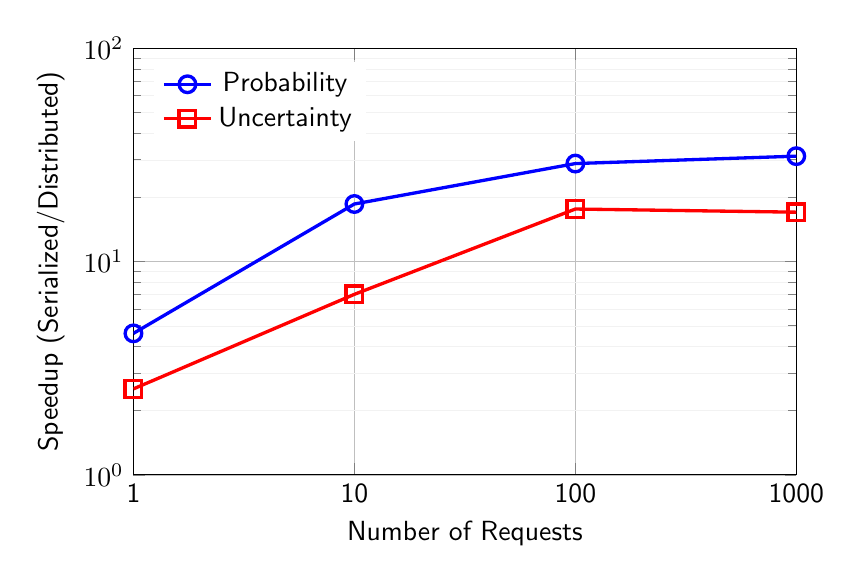
\begin{tikzpicture}
        \begin{loglogaxis}[
            width=10cm,
            height=7cm,
            grid=both,
            minor grid style={line width=.1pt, draw=gray!10},
            major grid style={line width=.2pt, draw=gray!50},
            xlabel={Number of Requests},
            ylabel={Speedup (Serialized/Distributed)},
            legend pos=north west,
            legend style={draw=none},
            xtick={1,10,100,1000},
            xticklabels={1,10,100,1000},
            log basis x=10,
            log basis y=10,
            ymin=1, ymax=100,
            xmin=1, xmax=1000
            ]
            
            % Probability speedup data
            \addplot[
                color=blue,
                mark=o,
                line width=1.2pt,
                mark size=3pt
                ] coordinates {
                (1, 4.603)
                (10, 18.6)
                (100, 28.776)
                (1000, 31.167)
            };
            
            % Uncertainty speedup data
            \addplot[
                color=red,
                mark=square,
                line width=1.2pt,
                mark size=3pt
                ] coordinates {
                (1, 2.528)
                (10, 7.016)
                (100, 17.616)
                (1000, 17.029)
            };
            
            \legend{Probability, Uncertainty}
        \end{loglogaxis}
    \end{tikzpicture}
    \caption{Speedup comparison between serialized and distributed execution for different request volumes.}
    \label{fig:speedup}
\end{figure}

The super-linear speedup for single request workloads is caused by the elimination of I/O processes. In the serialized \texttt{scram-cli} baseline, each run must (i) parse command-line arguments, (ii) read and validate the input XML fault-tree, (iii) launch a new process to execute the solver, and (iv) synchronously write results back to disk. In the distributed implementation, the request payload already contains the model and run-time parameters, which are passed directly to a Node.js native addon that invokes the underlying \texttt{scram} library. Result persistence is off-loaded to an asynchronous database writing process. So, both the initial XML parsing and the final file output are effectively removed from the process. Consequently, execution time reflects only the core solver computation, producing the observed speed-ups ($S\approx4.6$ for probability estimation and $S\approx2.5$ for uncertainty analysis) even at a single concurrent request.  
Beyond 100 jobs, speed-up saturates owing to:

\begin{itemize}
  \item \textbf{Worker saturation}: eight containers fully occupy the host's 8 hardware threads; adding jobs only increases wait time.
  \item \textbf{Queue latency}: larger batches incur longer residence times in RabbitMQ prior to dispatch.
  \item \textbf{Memory bandwidth limits}: uncertainty calculations are memory-bound; waiting time grows with concurrency.
\end{itemize}

These findings validate that the combined architecture of Docker-Swarm and RabbitMQ delivers near-linear scaling for practical PRA workloads up to the tested concurrency and provides an order-of-magnitude reduction in wall-clock time compared with serialized execution.
}

% \section{Handling Multi-Hazard Models in Parallel}
% \subsection{Integration of Hazard Modules}
% \subsection{Numerical Stability and Overflow Handling}

% \section{Security and Data Ownership}
% \subsection{Data Sharing Protocols}
% \subsection{Access Control and Regulatory Constraints}

\backmatter

% \section*{Listing the \texttt{LatexMk} file}
% \verbatiminput{./LatexMk}
\end{document}
